
\begin{DoxyItemize}
\item \hyperlink{handle_axes}{A\-X\-E\-S Create Handle Axes}  
\item \hyperlink{handle_axis}{A\-X\-I\-S Setup Axis Behavior}  
\item \hyperlink{handle_axisproperties}{A\-X\-I\-S\-P\-R\-O\-P\-E\-R\-T\-I\-E\-S Axis Object Properties}  
\item \hyperlink{handle_cla}{C\-L\-A Clear Current Axis}  
\item \hyperlink{handle_clabel}{C\-L\-A\-B\-E\-L Add Labels To Contour Plot}  
\item \hyperlink{handle_clf}{C\-L\-F Clear Figure}  
\item \hyperlink{handle_clim}{C\-L\-I\-M Adjust Color limits of plot}  
\item \hyperlink{handle_close}{C\-L\-O\-S\-E Close Figure Window}  
\item \hyperlink{handle_colorbar}{C\-O\-L\-O\-R\-B\-A\-R Add Colorbar to Current Plot}  
\item \hyperlink{handle_colormap}{C\-O\-L\-O\-R\-M\-A\-P Image Colormap Function}  
\item \hyperlink{handle_colorspec}{C\-O\-L\-O\-R\-S\-P\-E\-C Color Property Description}  
\item \hyperlink{handle_contour}{C\-O\-N\-T\-O\-U\-R Contour Plot Function}  
\item \hyperlink{handle_contour3}{C\-O\-N\-T\-O\-U\-R3 3\-D Contour Plot Function}  
\item \hyperlink{handle_copper}{C\-O\-P\-P\-E\-R Copper Colormap}  
\item \hyperlink{handle_copy}{C\-O\-P\-Y Copy Figure Window}  
\item \hyperlink{handle_countour}{C\-O\-U\-N\-T\-O\-U\-R Contour Object Properties}  
\item \hyperlink{handle_datacursormode}{D\-A\-T\-A\-C\-U\-R\-S\-O\-R\-M\-O\-D\-E Interactive Data Cursor}  
\item \hyperlink{handle_drawnow}{D\-R\-A\-W\-N\-O\-W Flush the Event Queue}  
\item \hyperlink{handle_figlower}{F\-I\-G\-L\-O\-W\-E\-R Lower a Figure Window}  
\item \hyperlink{handle_figraise}{F\-I\-G\-R\-A\-I\-S\-E Raise a Figure Window}  
\item \hyperlink{handle_figure}{F\-I\-G\-U\-R\-E Figure Window Select and Create Function}  
\item \hyperlink{handle_figureproperties}{F\-I\-G\-U\-R\-E\-P\-R\-O\-P\-E\-R\-T\-I\-E\-S Figure Object Properties}  
\item \hyperlink{handle_gca}{G\-C\-A Get Current Axis}  
\item \hyperlink{handle_gcf}{G\-C\-F Get Current Figure}  
\item \hyperlink{handle_get}{G\-E\-T Get Object Property}  
\item \hyperlink{handle_glshow}{G\-L\-S\-H\-O\-W Show a G\-L Assembly in a G\-L Window}  
\item \hyperlink{handle_gray}{G\-R\-A\-Y Gray Colormap}  
\item \hyperlink{handle_grid}{G\-R\-I\-D Plot Grid Toggle Function}  
\item \hyperlink{handle_hcontour}{H\-C\-O\-N\-T\-O\-U\-R Create a contour object}  
\item \hyperlink{handle_himage}{H\-I\-M\-A\-G\-E Create a image object}  
\item \hyperlink{handle_hist}{H\-I\-S\-T Histogram Function}  
\item \hyperlink{handle_hline}{H\-L\-I\-N\-E Create a line object}  
\item \hyperlink{handle_hold}{H\-O\-L\-D Plot Hold Toggle Function}  
\item \hyperlink{handle_hpatch}{H\-P\-A\-T\-C\-H Create a patch object}  
\item \hyperlink{handle_hpoint}{H\-P\-O\-I\-N\-T Get Point From Window}  
\item \hyperlink{handle_hrawplot}{H\-R\-A\-W\-P\-L\-O\-T Generate a Raw Plot File}  
\item \hyperlink{handle_hsurface}{H\-S\-U\-R\-F\-A\-C\-E Create a surface object}  
\item \hyperlink{handle_htext}{H\-T\-E\-X\-T Create a text object}  
\item \hyperlink{handle_htextbitmap}{H\-T\-E\-X\-T\-B\-I\-T\-M\-A\-P Get Text Rendered as a Bitmap}  
\item \hyperlink{handle_image}{I\-M\-A\-G\-E Image Display Function}  
\item \hyperlink{handle_imageproperties}{I\-M\-A\-G\-E\-P\-R\-O\-P\-E\-R\-T\-I\-E\-S Image Object Properties}  
\item \hyperlink{handle_imagesc}{I\-M\-A\-G\-E\-S\-C Image Display Function}  
\item \hyperlink{handle_is2dview}{I\-S2\-D\-V\-I\-E\-W Test Axes For 2\-D View}  
\item \hyperlink{handle_ishold}{I\-S\-H\-O\-L\-D Test Hold Status}  
\item \hyperlink{handle_legend}{L\-E\-G\-E\-N\-D Add Legent to Plot}  
\item \hyperlink{handle_line}{L\-I\-N\-E Line Display Function}  
\item \hyperlink{handle_lineproperties}{L\-I\-N\-E\-P\-R\-O\-P\-E\-R\-T\-I\-E\-S Line Series Object Properties}  
\item \hyperlink{handle_loglog}{L\-O\-G\-L\-O\-G Log-\/\-Log Plot Function}  
\item \hyperlink{handle_newplot}{N\-E\-W\-P\-L\-O\-T Get Handle For Next Plot}  
\item \hyperlink{handle_patch}{P\-A\-T\-C\-H Patch Graphics Function}  
\item \hyperlink{handle_pcolor}{P\-C\-O\-L\-O\-R Pseudocolor Plot}  
\item \hyperlink{handle_plot}{P\-L\-O\-T Plot Function}  
\item \hyperlink{handle_plot3}{P\-L\-O\-T3 Plot 3\-D Function}  
\item \hyperlink{handle_point}{P\-O\-I\-N\-T Get Axis Position From Mouse Click}  
\item \hyperlink{handle_print}{P\-R\-I\-N\-T Print a Figure To A File}  
\item \hyperlink{handle_pvalid}{P\-V\-A\-L\-I\-D Validate Property Name}  
\item \hyperlink{handle_semilogx}{S\-E\-M\-I\-L\-O\-G\-X Semilog X Axis Plot Function}  
\item \hyperlink{handle_semilogy}{S\-E\-M\-I\-L\-O\-G\-Y Semilog Y Axis Plot Function}  
\item \hyperlink{handle_set}{S\-E\-T Set Object Property}  
\item \hyperlink{handle_sizefig}{S\-I\-Z\-E\-F\-I\-G Set Size of Figure}  
\item \hyperlink{handle_subplot}{S\-U\-B\-P\-L\-O\-T Subplot Function}  
\item \hyperlink{handle_surf}{S\-U\-R\-F Surface Plot Function}  
\item \hyperlink{handle_surfaceproperties}{S\-U\-R\-F\-A\-C\-E\-P\-R\-O\-P\-E\-R\-T\-I\-E\-S Surface Object Properties}  
\item \hyperlink{handle_text}{T\-E\-X\-T Add Text Label to Plot}  
\item \hyperlink{handle_textproperties}{T\-E\-X\-T\-P\-R\-O\-P\-E\-R\-T\-I\-E\-S Text Object Properties}  
\item \hyperlink{handle_title}{T\-I\-T\-L\-E Plot Title Function}  
\item \hyperlink{handle_tubeplot}{T\-U\-B\-E\-P\-L\-O\-T Creates a Tubeplot}  
\item \hyperlink{handle_uicontrol}{U\-I\-C\-O\-N\-T\-R\-O\-L Create a U\-I Control object}  
\item \hyperlink{handle_uicontrolproperties}{U\-I\-C\-O\-N\-T\-R\-O\-L\-P\-R\-O\-P\-E\-R\-T\-I\-E\-S U\-I Control Properties}  
\item \hyperlink{handle_view}{V\-I\-E\-W Set Graphical View}  
\item \hyperlink{handle_winlev}{W\-I\-N\-L\-E\-V Image Window-\/\-Level Function}  
\item \hyperlink{handle_xlabel}{X\-L\-A\-B\-E\-L Plot X-\/axis Label Function}  
\item \hyperlink{handle_xlim}{X\-L\-I\-M Adjust X Axis limits of plot}  
\item \hyperlink{handle_ylabel}{Y\-L\-A\-B\-E\-L Plot Y-\/axis Label Function}  
\item \hyperlink{handle_ylim}{Y\-L\-I\-M Adjust Y Axis limits of plot}  
\item \hyperlink{handle_zlabel}{Z\-L\-A\-B\-E\-L Plot Z-\/axis Label Function}  
\item \hyperlink{handle_zlim}{Z\-L\-I\-M Adjust Z Axis limits of plot}  
\item \hyperlink{handle_zoom}{Z\-O\-O\-M Image Zoom Function}  
\item \hyperlink{handle_zplane}{Z\-P\-L\-A\-N\-E Zero-\/pole plot}  
\end{DoxyItemize}\hypertarget{handle_axes}{}\section{A\-X\-E\-S Create Handle Axes}\label{handle_axes}
Section\-: \hyperlink{sec_handle}{Handle-\/\-Based Graphics} \hypertarget{vtkwidgets_vtkxyplotwidget_Usage}{}\subsection{Usage}\label{vtkwidgets_vtkxyplotwidget_Usage}
This function has three different syntaxes. The first takes no arguments, \begin{DoxyVerb}  h = axes
\end{DoxyVerb}
 and creates a new set of axes that are parented to the current figure (see {\ttfamily gcf}). The newly created axes are made the current axes (see {\ttfamily gca}) and are added to the end of the list of children for the current figure. The second form takes a set of property names and values \begin{DoxyVerb}  h = axes(propertyname,value,propertyname,value,...)
\end{DoxyVerb}
 Creates a new set of axes, and then sets the specified properties to the given value. This is a shortcut for calling {\ttfamily set(h,propertyname,value)} for each pair. The third form takes a handle as an argument \begin{DoxyVerb}  axes(handle)
\end{DoxyVerb}
 and makes {\ttfamily handle} the current axes, placing it at the head of the list of children for the current figure. \hypertarget{handle_axis}{}\section{A\-X\-I\-S Setup Axis Behavior}\label{handle_axis}
Section\-: \hyperlink{sec_handle}{Handle-\/\-Based Graphics} \hypertarget{vtkwidgets_vtkxyplotwidget_Usage}{}\subsection{Usage}\label{vtkwidgets_vtkxyplotwidget_Usage}
Control the axis behavior. There are several versions of the axis command based on what you would like the axis command to do. The first versions set scalings for the current plot. The general syntax for its use is \begin{DoxyVerb}  axis([xmin xmax ymin ymax zmin zmax cmin cmax])
\end{DoxyVerb}
 which sets the limits in the X, Y, Z and color axes. You can also set only the X, Y and Z axes\-: \begin{DoxyVerb}  axis([xmin xmax ymin ymax zmin zmax])
\end{DoxyVerb}
 or only the X and Y axes\-: \begin{DoxyVerb}  axis([xmin xmax ymin ymax])
\end{DoxyVerb}
 To retrieve the current axis limits, use the syntax \begin{DoxyVerb}  x = axis
\end{DoxyVerb}
 where {\ttfamily x} is a 4-\/vector for 2\-D plots, and a 6-\/vector for 3\-D plots.

There are a number of axis options supported by Free\-Mat. The first version sets the axis limits to be automatically selected by Free\-Mat for each dimension. This state is the default one for new axes created by Free\-Mat. \begin{DoxyVerb}  axis auto
\end{DoxyVerb}
 The next option sets all of the axis limits to {\ttfamily manual} mode. This state turns off automatic scaling of the axis based on the children of the current axis object. \begin{DoxyVerb}  axis manual
\end{DoxyVerb}
 The next option sets the axis limits to fit tightly around the data. \begin{DoxyVerb}  axis tight
\end{DoxyVerb}
 The next option adjusts the axis limits and plotbox aspect ratio so that the axis fills the position rectangle. \begin{DoxyVerb}  axis fill
\end{DoxyVerb}
 The next option puts the axis in matrix mode. This mode is equivalent to the standard mode, but with the vertical axis reversed. Thus, the origin of the coordinate system is at the top left corner of the plot. This mode makes plots of matrix elements look normal (i.\-e., an identity matrix goes from upper left to lower right). \begin{DoxyVerb}  axis ij
\end{DoxyVerb}
 The next option puts the axis in normal mode, with the origin at the lower left corner. \begin{DoxyVerb}  axis xy
\end{DoxyVerb}
 The next option sets the axis parameters (specifically the data aspect ratio) so that equal ticks on each axis represent equal length. In this mode, spheres look spherical insteal of ellipsoidal. \begin{DoxyVerb}  axis equal
\end{DoxyVerb}
 The next option is the same as {\ttfamily axis equal}, but sets the plot box to fit tightly around the data (so no background shows through). It is the best option to use when displaying images. \begin{DoxyVerb}  axis image
\end{DoxyVerb}
 The next option makes the axis box square. \begin{DoxyVerb}  axis square
\end{DoxyVerb}
 The next option restores many of the normal characteristics of the axis. In particular, it undoes the effects of {\ttfamily square} {\ttfamily image} and {\ttfamily equal} modes. \begin{DoxyVerb}  axis normal
\end{DoxyVerb}
 The next mode freezes axis properties so that 3\-D objects can be rotated properly. \begin{DoxyVerb}  axis vis3d
\end{DoxyVerb}
 The next mode turns off all labels, tick marks and background. \begin{DoxyVerb}  axis on
\end{DoxyVerb}
 The next mode turns on all labels, tick marks and background. \begin{DoxyVerb}  axis off
\end{DoxyVerb}
 The next mode is similar to {\ttfamily axis off}, but also repacks the figure as tightly as possible. The result is a plot box that takes up the entire {\ttfamily outerposition} vector. \begin{DoxyVerb}  axis maximal
\end{DoxyVerb}
 The {\ttfamily axis} command can also be applied to a particular axis (as opposed to the current axis as returned by {\ttfamily gca}) handle \begin{DoxyVerb}  axis(M,...)
\end{DoxyVerb}
 \hypertarget{handle_axisproperties}{}\section{A\-X\-I\-S\-P\-R\-O\-P\-E\-R\-T\-I\-E\-S Axis Object Properties}\label{handle_axisproperties}
Section\-: \hyperlink{sec_handle}{Handle-\/\-Based Graphics} \hypertarget{vtkwidgets_vtkxyplotwidget_Usage}{}\subsection{Usage}\label{vtkwidgets_vtkxyplotwidget_Usage}
Below is a summary of the properties for the axis. 
\begin{DoxyItemize}
\item {\ttfamily activepositionproperty} -\/ {\ttfamily four vector} -\/ Not used.  
\item {\ttfamily alim} -\/ {\ttfamily two vector} -\/ Controls the mapping of transparency. The vector {\ttfamily \mbox{[}a\-\_\-1,a\-\_\-2\mbox{]}}@ defines the scale for transparency. Plots then map {\ttfamily a\-\_\-1} to a completely opaque value, and {\ttfamily a\-\_\-2} to a completely transparent value. This mapping is applied to the alpha data of the plot data.  
\item {\ttfamily alimmode} -\/ {\ttfamily \{'auto','manual'\}} -\/ For {\ttfamily auto} mode, we map the alpha ranges of all objects in the plot to a full scale. For {\ttfamily manual} mode, we use the {\ttfamily alim} vector.  
\item {\ttfamily ambientlightcolor} -\/ {\ttfamily colorspec} -\/ Not used.  
\item {\ttfamily box} -\/ {\ttfamily On/\-Off} -\/ Not used.  
\item {\ttfamily cameraposition} -\/ {\ttfamily three vector} -\/ Set the position for the camera in axis space.  
\item {\ttfamily camerapositionmode} -\/ {\ttfamily \{'auto','manual'\}} -\/ For {\ttfamily manual} mode, the camera position is picked up from the {\ttfamily cameraposition} vector. For {\ttfamily auto} mode, the camera position is set to be centered on the {\ttfamily x} and {\ttfamily y} axis limits, and beyond the {\ttfamily z} maximum limit.  
\item {\ttfamily cameratarget} -\/ {\ttfamily three vector} -\/ Defines the point in axis space that the camera is targetted at.  
\item {\ttfamily cameratargetmode} -\/ {\ttfamily \{'auto','manual'\}} -\/ For {\ttfamily manual} mode the camera target is picked up from the {\ttfamily cameratarget} vector. For {\ttfamily auto} mode, the camera target is chosen to be the center of the three axes.  
\item {\ttfamily cameraupvector} -\/ {\ttfamily three vector} -\/ Defines the upwards vector for the camera (what is ultimately mapped to the vertical axis of the plot or screen). This vector must not be parallel to the vector that is defined by the optical axis (i.\-e., the one connecting the target to the camera position).  
\item {\ttfamily cameraupvectormode} -\/ {\ttfamily \{'auto','manual'\}} -\/ For {\ttfamily manual} mode, the camera up vector is picked up from the {\ttfamily cameraupvector}. The {\ttfamily auto} mode chooses the up vector to point along the positive {\ttfamily y} axis.  
\item {\ttfamily cameraviewangle} -\/ {\ttfamily scalar} -\/ Not used.  
\item {\ttfamily cameraviewanglemode} -\/ {\ttfamily \{'auto','manual'\}} -\/ Not used.  
\item {\ttfamily children} -\/ {\ttfamily vector of handles} -\/ A vector containing handles to children of the current axis. Be careful as to how you manipulate this vector. Free\-Mat uses a reference counting mechanism for graphics objects, so if you remove a handle from the {\ttfamily children} property of an axis, and you have not added it to the {\ttfamily children} property of another object, it will be deleted.  
\item {\ttfamily clim} -\/ {\ttfamily two vector} -\/ The color range vector. This vector contains two values that dictate how children of this axis get mapped to the colormap. Values between the two endpoints of this vector are mapped to the extremes of the colormap.  
\item {\ttfamily climmode} -\/ {\ttfamily \{'auto','manual'\}} -\/ For {\ttfamily auto} mode, the color limits are chosen to span the colordata for all of the children objects. For {\ttfamily manual} mode, the color mapping is based on {\ttfamily clim}.  
\item {\ttfamily clipping} -\/ {\ttfamily \{'on','off'\}} -\/ Not used.  
\item {\ttfamily color} -\/ {\ttfamily colorspec} -\/ The color used to draw the background box for the axes. Defaults to white.  
\item {\ttfamily colororder} -\/ {\ttfamily color vector} -\/ A vector of color specs (in R\-G\-B) that are cycled between when drawing line plots into this axis. The default is order blue,green,red,cyan,magenta,yellow,black.  
\item {\ttfamily datalimits} -\/ {\ttfamily six vector} -\/ A vector that contains the x, y and z limits of the data for children of the current axis. Changes to this property are ignored -\/ it is calculated by Free\-Mat based on the datasets.  
\item {\ttfamily dataaspectratio} -\/ {\ttfamily three vector} -\/ A vector that describes the aspect ratio of the data. You can think of this as the relative scaling of units for each axis. For example, if one unit along the x axis is twice as long as one unit along the y axis, you would specify a data aspect ratio of {\ttfamily \mbox{[}2,1,1\mbox{]}}.  
\item {\ttfamily dataaspectratiomode} -\/ {\ttfamily \{'auto','manual'\}} -\/ When the data aspect ratio is set to {\ttfamily manual}, the data is scaled by the data aspect ratio before being plotted. When the data aspect ratio mode is {\ttfamily auto} a complex set of rules are applied to determine how the data should be scaled. If {\ttfamily dataaspectratio} mode is {\ttfamily auto} and {\ttfamily plotboxaspectratio} is {\ttfamily auto}, then the default data aspect ratio is set to {\ttfamily \mbox{[}1,1,1\mbox{]}} and the default plot box aspect ratio is chosen proportional to {\ttfamily \mbox{[}xrange,yrange,zrange\mbox{]}}, where {\ttfamily xrange} is the span of data along the {\ttfamily x} axis, and similarly for {\ttfamily yrange} and {\ttfamily zrange}. If {\ttfamily plotboxaspectratio} is set to {\ttfamily \mbox{[}px,py,pz\mbox{]}}, then the {\ttfamily dataaspectratio} is set to {\ttfamily \mbox{[}xrange/px,yrange/py,zrange/pz\mbox{]}}. If one of the axes has been specified manually, then the data will be scaled to fit the axes as well as possible.  
\item {\ttfamily fontangle} -\/ {\ttfamily \{'normal','italic','oblique'\}} -\/ The angle of the fonts used for text labels (e.\-g., tick labels).  
\item {\ttfamily fontsize} -\/ {\ttfamily scalar} -\/ The size of fonts used for text labels (tick labels).  
\item {\ttfamily fontunits} -\/ Not used.  
\item {\ttfamily fontweight} -\/ {\ttfamily \{'normal','bold','light','demi'\}} -\/ The weight of the font used for tick labels.  
\item {\ttfamily gridlinestyle} -\/ {\ttfamily \{'-\/','--','\-:','-\/.','none'\}} -\/ The line style to use for drawing the grid lines. Defaults to {\ttfamily '\-:'}.  
\item {\ttfamily handlevisibility} -\/ Not used.  
\item {\ttfamily hittest} -\/ Not used.  
\item {\ttfamily interruptible} -\/ Not used.  
\item {\ttfamily layer} -\/ Not used.  
\item {\ttfamily linestyleorder} -\/ {\ttfamily linestyle vector} -\/ A vector of linestyles that are cycled through when plotted line series.  
\item {\ttfamily linewidth} -\/ {\ttfamily scalar} -\/ The width of line used to draw grid lines, axis lines, and other lines.  
\item {\ttfamily minorgridlinestyle} -\/ {\ttfamily \{'-\/','--','\-:','-\/.','none'\}} -\/ The line style used for drawing grid lines through minor ticks.  
\item {\ttfamily nextplot} -\/ {\ttfamily \{'add','replace','replacechildren'\}} -\/ Controls how the next plot interacts with the axis. If it is set to {\ttfamily 'add'} the next plot will be added to the current axis. If it is set to {\ttfamily 'replace'} the new plot replaces all of the previous children.  
\item {\ttfamily outerposition} -\/ {\ttfamily four vector} -\/ Specifies the coordinates of the outermost box that contains the axis relative to the containing figure. This vector is in normalized coordinates and corresponds to the {\ttfamily x, y, width, height} coordinates of the box.  
\item {\ttfamily parent} -\/ {\ttfamily handle} -\/ The handle for the containing object (a figure).  
\item {\ttfamily plotboxaspectratio} -\/ {\ttfamily three vector} -\/ Controls the aspect ratio of the plot box. See the entry under {\ttfamily dataaspectratio} for details on how Free\-Mat uses this vector in combination with the axis limits and the {\ttfamily plotboxaspectratio} to determine how to scale the data.  
\item {\ttfamily plotboxaspectratiomode} -\/ {\ttfamily \{'auto','manual'\}} -\/ The plot box aspect ratio mode interacts with the {\ttfamily dataaspectratiomode} and the axis limits.  
\item {\ttfamily position} -\/ {\ttfamily fourvector} -\/ The normalized coordinates of the plot box space. Should be inside the rectable defined by {\ttfamily outerposition}.  
\item {\ttfamily positionmode} -\/ {\ttfamily \{'auto','manual'\}} -\/ the position mode is normally {\ttfamily 'auto'} which means that Free\-Mat computes the position vector to fit the plot inside the {\ttfamily outerposition} vector. If you set the {\ttfamily position} vector manually (using a {\ttfamily set} command), this {\ttfamily mode} flag becomes {\ttfamily 'manual'} and remains that way until reset to @$|$'auto'.  
\item {\ttfamily projection} -\/ Not used.  
\item {\ttfamily selected} -\/ Not used.  
\item {\ttfamily selectionhighlight} -\/ Not used.  
\item {\ttfamily tag} -\/ A string that can be set to tag the axes with a name.  
\item {\ttfamily textheight} -\/ {\ttfamily scalar} -\/ This value is set by Free\-Mat to the height of the current font in pixels.  
\item {\ttfamily tickdir} -\/ {\ttfamily \{'in','out'\}} -\/ The direction of ticks. Defaults to {\ttfamily 'in'} for 2\-D plots, and {\ttfamily 'out'} for 3\-D plots if {\ttfamily tickdirmode} is {\ttfamily auto}.  
\item {\ttfamily tickdirmode} -\/ {\ttfamily \{'auto','manual'\}} -\/ When set to {\ttfamily 'auto'} the {\ttfamily tickdir} defaults to {\ttfamily 'in'} for 2\-D plots, and {\ttfamily 'out'} for 3\-D plots.  
\item {\ttfamily ticklength} -\/ {\ttfamily two vector} -\/ The first element is the length of the tick in 2\-D plots, and the second is the length of the tick in the 3\-D plots. The lengths are described as fractions of the longer dimension (width or height).  
\item {\ttfamily tightinset} -\/ Not used.  
\item {\ttfamily title} -\/ {\ttfamily handle} -\/ The handle of the label used to represent the title of the plot.  
\item {\ttfamily type} -\/ {\ttfamily string} -\/ Takes the value of {\ttfamily 'axes'} for objects of the axes type.  
\item {\ttfamily units} -\/ Not used.  
\item {\ttfamily userdata} -\/ {\ttfamily array} -\/ An arbitrary array you can set to anything you want.  
\item {\ttfamily visible} -\/ {\ttfamily \{'on','off'\}} -\/ If set to {\ttfamily 'on'} the axes are drawn as normal. If set to {\ttfamily 'off'}, only the children of the axes are drawn. The plot box, axis lines, and tick labels are not drawn.  
\item {\ttfamily xaxislocation} -\/ {\ttfamily \{'top','bottom'\}} -\/ Controls placement of the x axis.  
\item {\ttfamily yaxislocation} -\/ {\ttfamily \{'left','right'\}} -\/ Controls placement of the y axis.  
\item {\ttfamily xcolor} -\/ {\ttfamily colorspec} -\/ The color of the x elements including the the x axis line, ticks, grid lines and tick labels  
\item {\ttfamily ycolor} -\/ {\ttfamily colorspec} -\/ The color of the y elements including the the y axis line, ticks, grid lines and tick labels.  
\item {\ttfamily zcolor} -\/ {\ttfamily colorspec} -\/ The color of the z elements including the the z axis line, ticks, grid lines and tick labels.  
\item {\ttfamily xdir} -\/ {\ttfamily \{'normal','reverse'\}} -\/ For {\ttfamily normal}, axes are drawn as you would expect (e.\-g, in default 2\-D mode, the x axis has values increasing from left to right. For {\ttfamily reverse}, the x axis has values increasing from right to left.  
\item {\ttfamily ydir} -\/ {\ttfamily \{'normal','reverse'\}} -\/ For {\ttfamily normal}, axes are drawn as you would expect (e.\-g, in default 2\-D mode, the y axis has values increasing from bottom to top. For {\ttfamily reverse}, the y axis has values increasing from top to bottom.  
\item {\ttfamily zdir} -\/ {\ttfamily \{'normal','reverse'\}} -\/ For {\ttfamily normal}, axes are drawn as you would expect. In default 3\-D mode, the z axis has values increasing in some direction (usually up). For {\ttfamily reverse} the z axis increases in the opposite direction.  
\item {\ttfamily xgrid} -\/ {\ttfamily \{'on','off'\}} -\/ Set to {\ttfamily on} to draw grid lines from ticks on the x axis.  
\item {\ttfamily ygrid} -\/ {\ttfamily \{'on','off'\}} -\/ Set to {\ttfamily on} to draw grid lines from ticks on the y axis.  
\item {\ttfamily zgrid} -\/ {\ttfamily \{'on','off'\}} -\/ Set to {\ttfamily on} to draw grid lines from ticks on the z axis.  
\item {\ttfamily xlabel} -\/ {\ttfamily handle} -\/ The handle of the text label attached to the x axis. The position of that label and the rotation angle is computed automatically by Free\-Mat.  
\item {\ttfamily ylabel} -\/ {\ttfamily handle} -\/ The handle of the text label attached to the y axis. The position of that label and the rotation angle is computed automatically by Free\-Mat.  
\item {\ttfamily zlabel} -\/ {\ttfamily handle} -\/ The handle of the text label attached to the z axis. The position of that label and the rotation angle is computed automatically by Free\-Mat.  
\item {\ttfamily xlim} -\/ {\ttfamily two vector} -\/ Contains the limits of the data along the x axis. These are set automatically for {\ttfamily xlimmode}. When manually set it allows you to zoom into the data. The first element of this vector should be the smallest x value you want mapped to the axis, and the second element should be the largest.  
\item {\ttfamily ylim} -\/ {\ttfamily two vector} -\/ Contains the limits of the data along the y axis. These are set automatically for {\ttfamily ylimmode}. When manually set it allows you to zoom into the data. The first element of this vector should be the smallest y value you want mapped to the axis, and the second element should be the largest.  
\item {\ttfamily zlim} -\/ {\ttfamily two vector} -\/ Contains the limits of the data along the z axis. These are set automatically for {\ttfamily zlimmode}. When manually set it allows you to zoom into the data. The first element of this vector should be the smallest z value you want mapped to the axis, and the second element should be the largest.  
\item {\ttfamily xlimmode} -\/ {\ttfamily \{'auto','manual'\}} -\/ Determines if {\ttfamily xlim} is determined automatically or if it is determined manually. When determined automatically, it is chosen to span the data range (at least).  
\item {\ttfamily ylimmode} -\/ {\ttfamily \{'auto','manual'\}} -\/ Determines if {\ttfamily ylim} is determined automatically or if it is determined manually. When determined automatically, it is chosen to span the data range (at least).  
\item {\ttfamily zlimmode} -\/ {\ttfamily \{'auto','manual'\}} -\/ Determines if {\ttfamily zlim} is determined automatically or if it is determined manually. When determined automatically, it is chosen to span the data range (at least).  
\item {\ttfamily xminorgrid} -\/ {\ttfamily \{'on','off'\}} -\/ Set to {\ttfamily on} to draw grid lines from minor ticks on the x axis.  
\item {\ttfamily yminorgrid} -\/ {\ttfamily \{'on','off'\}} -\/ Set to {\ttfamily on} to draw grid lines from minor ticks on the y axis.  
\item {\ttfamily zminorgrid} -\/ {\ttfamily \{'on','off'\}} -\/ Set to {\ttfamily on} to draw grid lines from minor ticks on the z axis.  
\item {\ttfamily xscale} -\/ {\ttfamily \{'linear','log'\}} -\/ Determines if the data on the x axis is linear or logarithmically scaled.  
\item {\ttfamily yscale} -\/ {\ttfamily \{'linear','log'\}} -\/ Determines if the data on the y axis is linear or logarithmically scaled.  
\item {\ttfamily zscale} -\/ {\ttfamily \{'linear','log'\}} -\/ Determines if the data on the z axis is linear or logarithmically scaled.  
\item {\ttfamily xtick} -\/ {\ttfamily vector} -\/ A vector of x coordinates where ticks are placed on the x axis. Setting this vector allows you complete control over the placement of ticks on the axis.  
\item {\ttfamily ytick} -\/ {\ttfamily vector} -\/ A vector of y coordinates where ticks are placed on the y axis. Setting this vector allows you complete control over the placement of ticks on the axis.  
\item {\ttfamily ztick} -\/ {\ttfamily vector} -\/ A vector of z coordinates where ticks are placed on the z axis. Setting this vector allows you complete control over the placement of ticks on the axis.  
\item {\ttfamily xticklabel} -\/ {\ttfamily string vector} -\/ A string vector, of the form {\ttfamily 'string}string$|$string'$|$ that contains labels to assign to the labels on the axis. If this vector is shorter than {\ttfamily xtick}, then Free\-Mat will cycle through the elements of this vector to fill out the labels.  
\item {\ttfamily yticklabel} -\/ {\ttfamily string vector} -\/ A string vector, of the form {\ttfamily 'string}string$|$string'$|$ that contains labels to assign to the labels on the axis. If this vector is shorter than {\ttfamily ytick}, then Free\-Mat will cycle through the elements of this vector to fill out the labels.  
\item {\ttfamily zticklabel} -\/ {\ttfamily string vector} -\/ A string vector, of the form {\ttfamily 'string}string$|$string'$|$ that contains labels to assign to the labels on the axis. If this vector is shorter than {\ttfamily ztick}, then Free\-Mat will cycle through the elements of this vector to fill out the labels.  
\item {\ttfamily xtickmode} -\/ {\ttfamily \{'auto','manual'\}} -\/ Set to {\ttfamily 'auto'} if you want Free\-Mat to calculate the tick locations. Setting {\ttfamily 'xtick'} will cause this property to switch to {\ttfamily 'manual'}.  
\item {\ttfamily ytickmode} -\/ {\ttfamily \{'auto','manual'\}} -\/ Set to {\ttfamily 'auto'} if you want Free\-Mat to calculate the tick locations. Setting {\ttfamily 'ytick'} will cause this property to switch to {\ttfamily 'manual'}.  
\item {\ttfamily ztickmode} -\/ {\ttfamily \{'auto','manual'\}} -\/ Set to {\ttfamily 'auto'} if you want Free\-Mat to calculate the tick locations. Setting {\ttfamily 'ztick'} will cause this property to switch to {\ttfamily 'manual'}.  
\item {\ttfamily xticklabelmode} -\/ {\ttfamily \{'auto','manual'\}} -\/ Set to {\ttfamily 'auto'} if you want Free\-Mat to set the tick labels. This will be based on the vector {\ttfamily xtick}.  
\item {\ttfamily yticklabelmode} -\/ {\ttfamily \{'auto','manual'\}} -\/ Set to {\ttfamily 'auto'} if you want Free\-Mat to set the tick labels. This will be based on the vector {\ttfamily ytick}.  
\item {\ttfamily zticklabelmode} -\/ {\ttfamily \{'auto','manual'\}} -\/ Set to {\ttfamily 'auto'} if you want Free\-Mat to set the tick labels. This will be based on the vector {\ttfamily ztick}.  
\end{DoxyItemize}\hypertarget{handle_cla}{}\section{C\-L\-A Clear Current Axis}\label{handle_cla}
Section\-: \hyperlink{sec_handle}{Handle-\/\-Based Graphics} \hypertarget{vtkwidgets_vtkxyplotwidget_Usage}{}\subsection{Usage}\label{vtkwidgets_vtkxyplotwidget_Usage}
Clears the current axes. The syntax for its use is \begin{DoxyVerb}  cla
\end{DoxyVerb}
 \hypertarget{handle_clabel}{}\section{C\-L\-A\-B\-E\-L Add Labels To Contour Plot}\label{handle_clabel}
Section\-: \hyperlink{sec_handle}{Handle-\/\-Based Graphics} \hypertarget{vtkwidgets_vtkxyplotwidget_Usage}{}\subsection{Usage}\label{vtkwidgets_vtkxyplotwidget_Usage}
The {\ttfamily clabel} function adds labels to a contour plot Generate contour labels for a contour plot. The syntax for its use is either\-: \begin{DoxyVerb}   handles = clabel(contourhandle,property,value,property,value,...)
\end{DoxyVerb}
 which labels all of the contours in the plot, or \begin{DoxyVerb}   handles = clabel(contourhandle,vals,property,value,property,value,...)
\end{DoxyVerb}
 which only labels those contours indicated by the vector {\ttfamily vals}. The {\ttfamily contourhandle} must be the handle to a contour plot object. The remaining property/value pairs are passed to the {\ttfamily text} function to control the parameters of the generated text labels. See the {\ttfamily text properties} for the details on what can be used in those labels. \hypertarget{variables_struct_Example}{}\subsection{Example}\label{variables_struct_Example}

\begin{DoxyVerbInclude}
--> [x,y] = meshgrid(linspace(-1,1,50));
--> z = x.*exp(-(x.^2+y.^2));
--> h = contour(z);
--> clabel(h,'backgroundcolor',[1,1,.6],'edgecolor',[.7,.7,.7]);
\end{DoxyVerbInclude}


which results in  
\begin{DoxyImage}
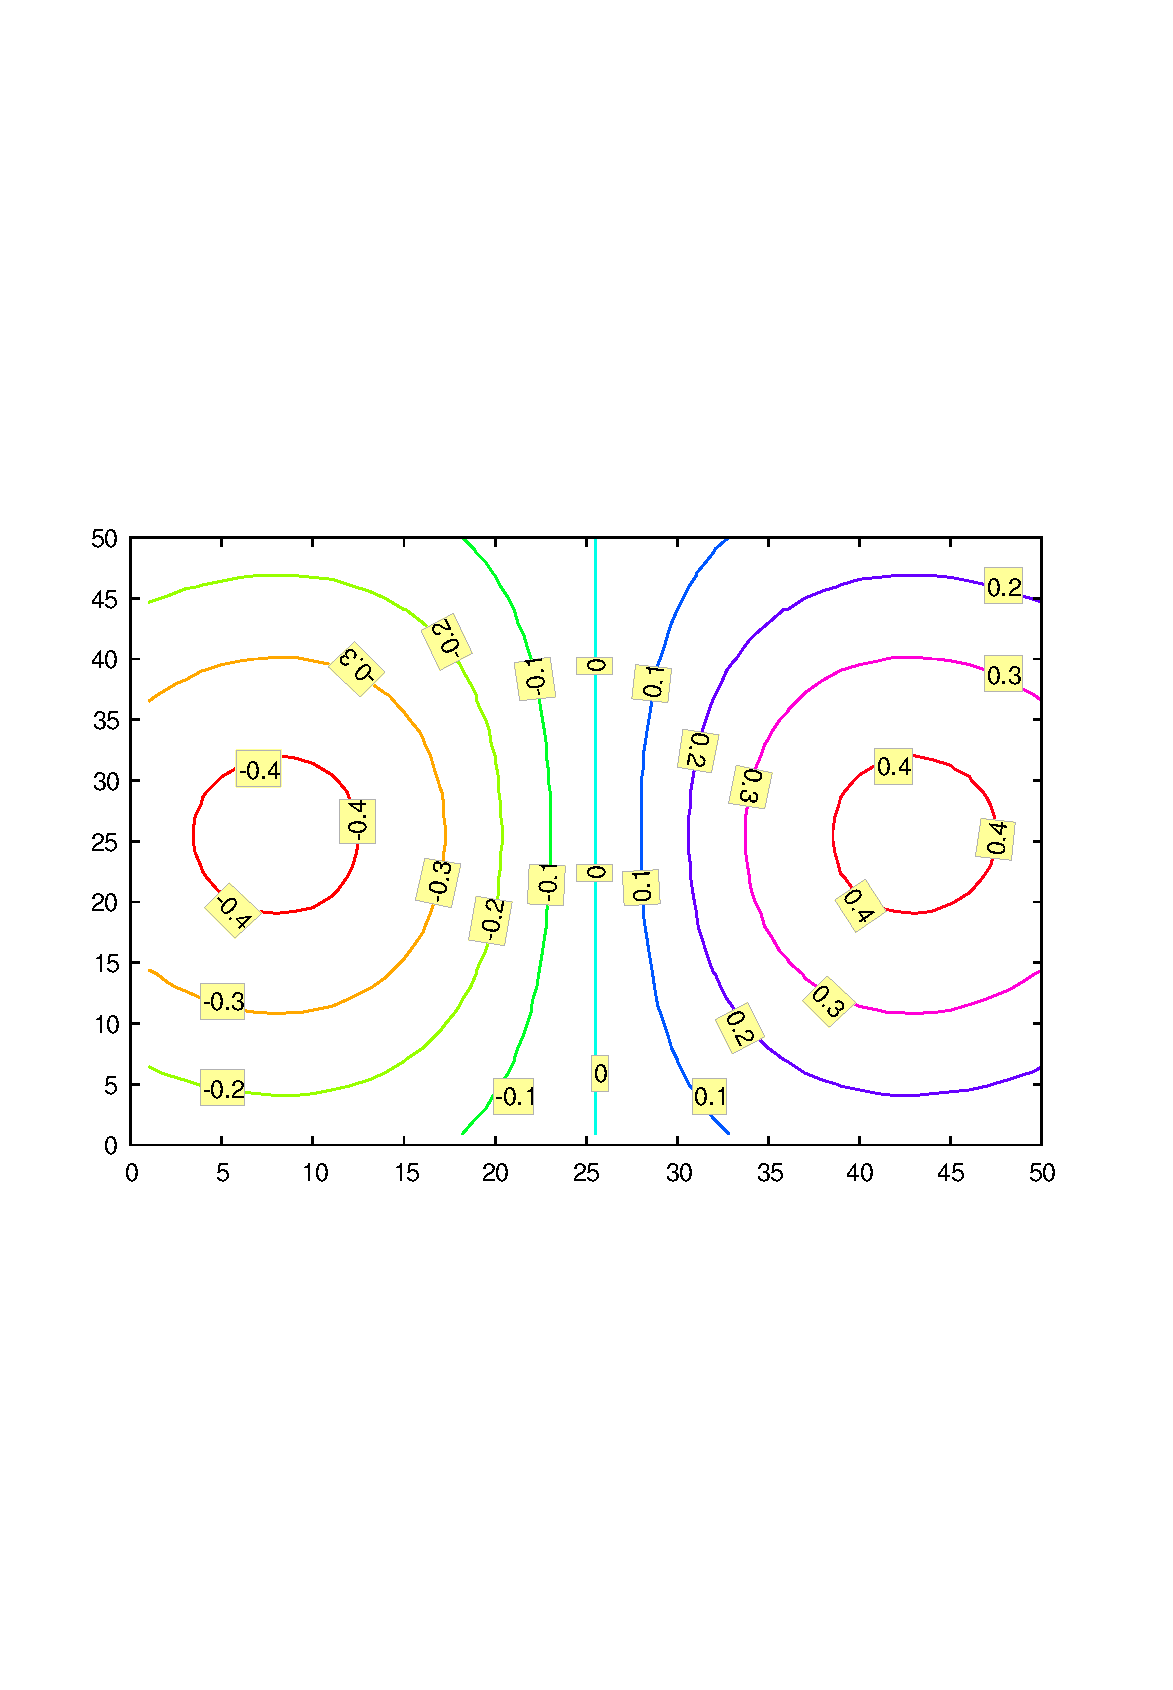
\includegraphics[width=12cm]{clabel1}
\caption{clabel1}
\end{DoxyImage}
 Alternately, we can just label a subset of the contours


\begin{DoxyVerbInclude}
--> h = contour(z);
--> clabel(h,[-.2,0,.3]);
\end{DoxyVerbInclude}


which results in  
\begin{DoxyImage}
\includegraphics[width=12cm]{clabel2}
\caption{clabel2}
\end{DoxyImage}
 \hypertarget{handle_clf}{}\section{C\-L\-F Clear Figure}\label{handle_clf}
Section\-: \hyperlink{sec_handle}{Handle-\/\-Based Graphics} \hypertarget{vtkwidgets_vtkxyplotwidget_Usage}{}\subsection{Usage}\label{vtkwidgets_vtkxyplotwidget_Usage}
This function clears the contents of the current figure. The syntax for its use is \begin{DoxyVerb}   clf
\end{DoxyVerb}
 \hypertarget{handle_clim}{}\section{C\-L\-I\-M Adjust Color limits of plot}\label{handle_clim}
Section\-: \hyperlink{sec_handle}{Handle-\/\-Based Graphics} \hypertarget{vtkwidgets_vtkxyplotwidget_Usage}{}\subsection{Usage}\label{vtkwidgets_vtkxyplotwidget_Usage}
There are several ways to use {\ttfamily clim} to adjust the color limits of a plot. The various syntaxes are \begin{DoxyVerb}   clim
   clim([lo,hi])   
   clim('auto')
   clim('manual')
   clim('mode')
   clim(handle,...)
\end{DoxyVerb}
 The first form (without arguments), returns a 2-\/vector containing the current limits. The second form sets the limits on the plot to {\ttfamily \mbox{[}lo,hi\mbox{]}}. The third and fourth form set the mode for the limit to {\ttfamily auto} and {\ttfamily manual} respectively. In {\ttfamily auto} mode, Free\-Mat chooses the range for the axis automatically. The {\ttfamily clim('mode')} form returns the current mode for the axis (either {\ttfamily 'auto'} or {\ttfamily 'manual'}).

Switching to {\ttfamily manual} mode does not change the limits, it simply allows you to modify them (and disables the automatic adjustment of the limits as more objects are added to the plot). Also, if you specify a set of limits explicitly, the mode is set to {\ttfamily manual}

Finally, you can specify the handle of an axis to manipulate instead of using the current one. \hypertarget{variables_struct_Example}{}\subsection{Example}\label{variables_struct_Example}
Here is an example of using {\ttfamily clim} to change the effective window and level onto an image. First, the image with default limits


\begin{DoxyVerbInclude}
--> x = repmat(linspace(-1,1),[100,1]); y = x';
--> z = exp(-x.^2-y.^2);
--> image(z);
--> min(z(:))

ans = 
    0.1353 

--> max(z(:))

ans = 
    0.9998 
\end{DoxyVerbInclude}


which results in  
\begin{DoxyImage}
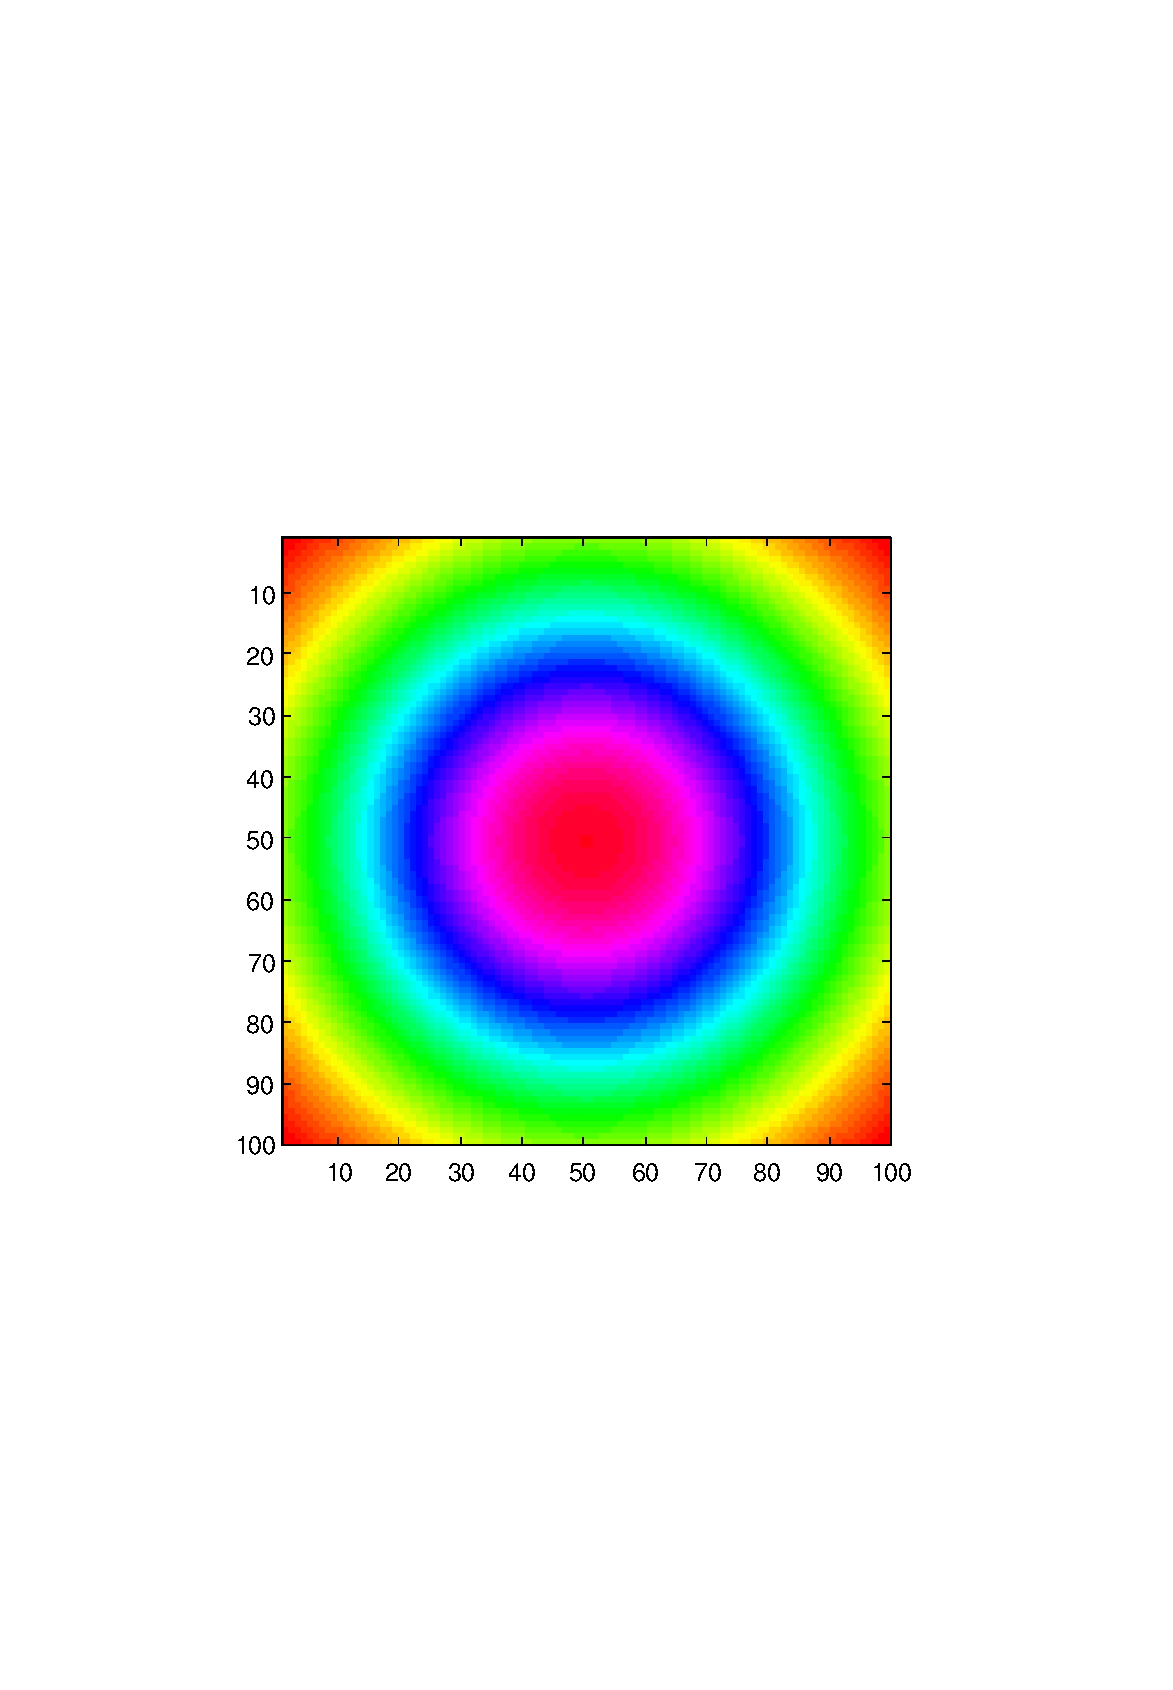
\includegraphics[width=12cm]{clim1}
\caption{clim1}
\end{DoxyImage}
 Next, we change the colorscale of the image using the {\ttfamily clim} function


\begin{DoxyVerbInclude}
--> image(z);
--> clim([0,0.2]);
\end{DoxyVerbInclude}


which results in  
\begin{DoxyImage}
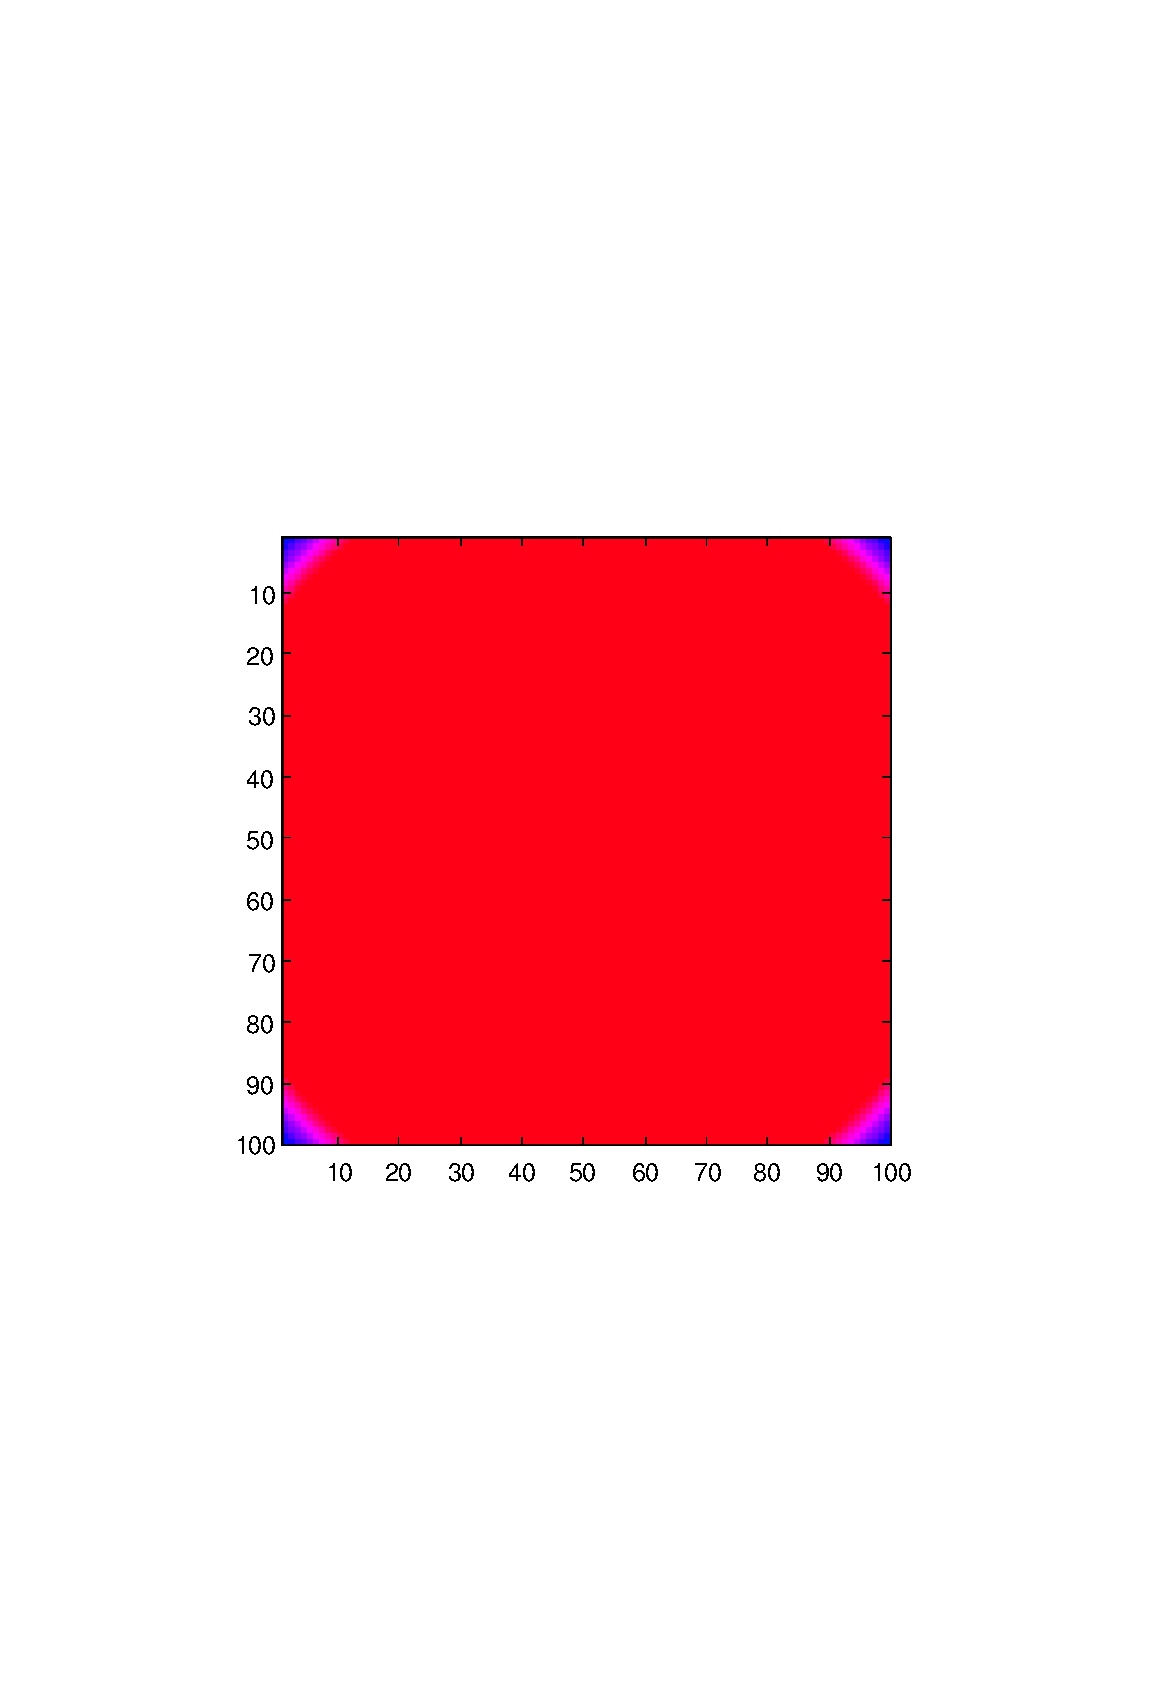
\includegraphics[width=12cm]{clim2}
\caption{clim2}
\end{DoxyImage}
 \hypertarget{handle_close}{}\section{C\-L\-O\-S\-E Close Figure Window}\label{handle_close}
Section\-: \hyperlink{sec_handle}{Handle-\/\-Based Graphics} \hypertarget{vtkwidgets_vtkxyplotwidget_Usage}{}\subsection{Usage}\label{vtkwidgets_vtkxyplotwidget_Usage}
Closes a figure window, either the currently active window, a window with a specific handle, or all figure windows. The general syntax for its use is \begin{DoxyVerb}   close(handle)
\end{DoxyVerb}
 in which case the figure window with the speicified {\ttfamily handle} is closed. Alternately, issuing the command with no argument \begin{DoxyVerb}   close
\end{DoxyVerb}
 is equivalent to closing the currently active figure window. Finally the command \begin{DoxyVerb}   close('all')
\end{DoxyVerb}
 closes all figure windows currently open. \hypertarget{handle_colorbar}{}\section{C\-O\-L\-O\-R\-B\-A\-R Add Colorbar to Current Plot}\label{handle_colorbar}
Section\-: \hyperlink{sec_handle}{Handle-\/\-Based Graphics} \hypertarget{vtkwidgets_vtkxyplotwidget_Usage}{}\subsection{Usage}\label{vtkwidgets_vtkxyplotwidget_Usage}
There are a number of syntaxes for the {\ttfamily colorbar} command. The first takes no arguments, and adds a vertical colorbar to the right of the current axes. \begin{DoxyVerb}  colorbar
\end{DoxyVerb}
 You can also pass properties to the newly created axes object using the second syntax for colorbar \begin{DoxyVerb}  colorbar(properties...)
\end{DoxyVerb}
 \hypertarget{handle_colormap}{}\section{C\-O\-L\-O\-R\-M\-A\-P Image Colormap Function}\label{handle_colormap}
Section\-: \hyperlink{sec_handle}{Handle-\/\-Based Graphics} \hypertarget{vtkwidgets_vtkxyplotwidget_Usage}{}\subsection{Usage}\label{vtkwidgets_vtkxyplotwidget_Usage}
Changes the colormap for the current figure. The generic syntax for its use is \begin{DoxyVerb}  colormap(map)
\end{DoxyVerb}
 where {\ttfamily map} is a an array organized as $3 \times N$), which defines the R\-G\-B (Red Green Blue) coordinates for each color in the colormap. You can also use the function with no arguments to recover the current colormap \begin{DoxyVerb}  map = colormap
\end{DoxyVerb}
 \hypertarget{transforms_svd_Function}{}\subsection{Internals}\label{transforms_svd_Function}
Assuming that the contents of the colormap function argument {\ttfamily c} are labeled as\-: \[ c = \begin{bmatrix} r_1 & g_1 & b_1 \\ r_1 & g_2 & b_2 \\ r_1 & g_3 & b_3 \\ \vdots & \vdots & \vdots \end{bmatrix} \] then these columns for the R\-G\-B coordinates of pixel in the mapped image. Assume that the image occupies the range \$\mbox{[}a,b\mbox{]}\$. Then the R\-G\-B color of each pixel depends on the value \$x\$ via the following integer \[ k = 1 + \lfloor 256 \frac{x-a}{b-a} \rfloor, \] so that a pixel corresponding to image value \$x\$ will receive R\-G\-B color \$\mbox{[}r\-\_\-k,g\-\_\-k,b\-\_\-k\mbox{]}\$. Colormaps are generally used to pseudo color images to enhance visibility of features, etc. \hypertarget{variables_matrix_Examples}{}\subsection{Examples}\label{variables_matrix_Examples}
We start by creating a smoothly varying image of a 2\-D Gaussian pulse.


\begin{DoxyVerbInclude}
--> x = linspace(-1,1,512)'*ones(1,512);
--> y = x';
--> Z = exp(-(x.^2+y.^2)/0.3);
--> image(Z);
\end{DoxyVerbInclude}


which we display with the default (grayscale) colormap here.  
\begin{DoxyImage}
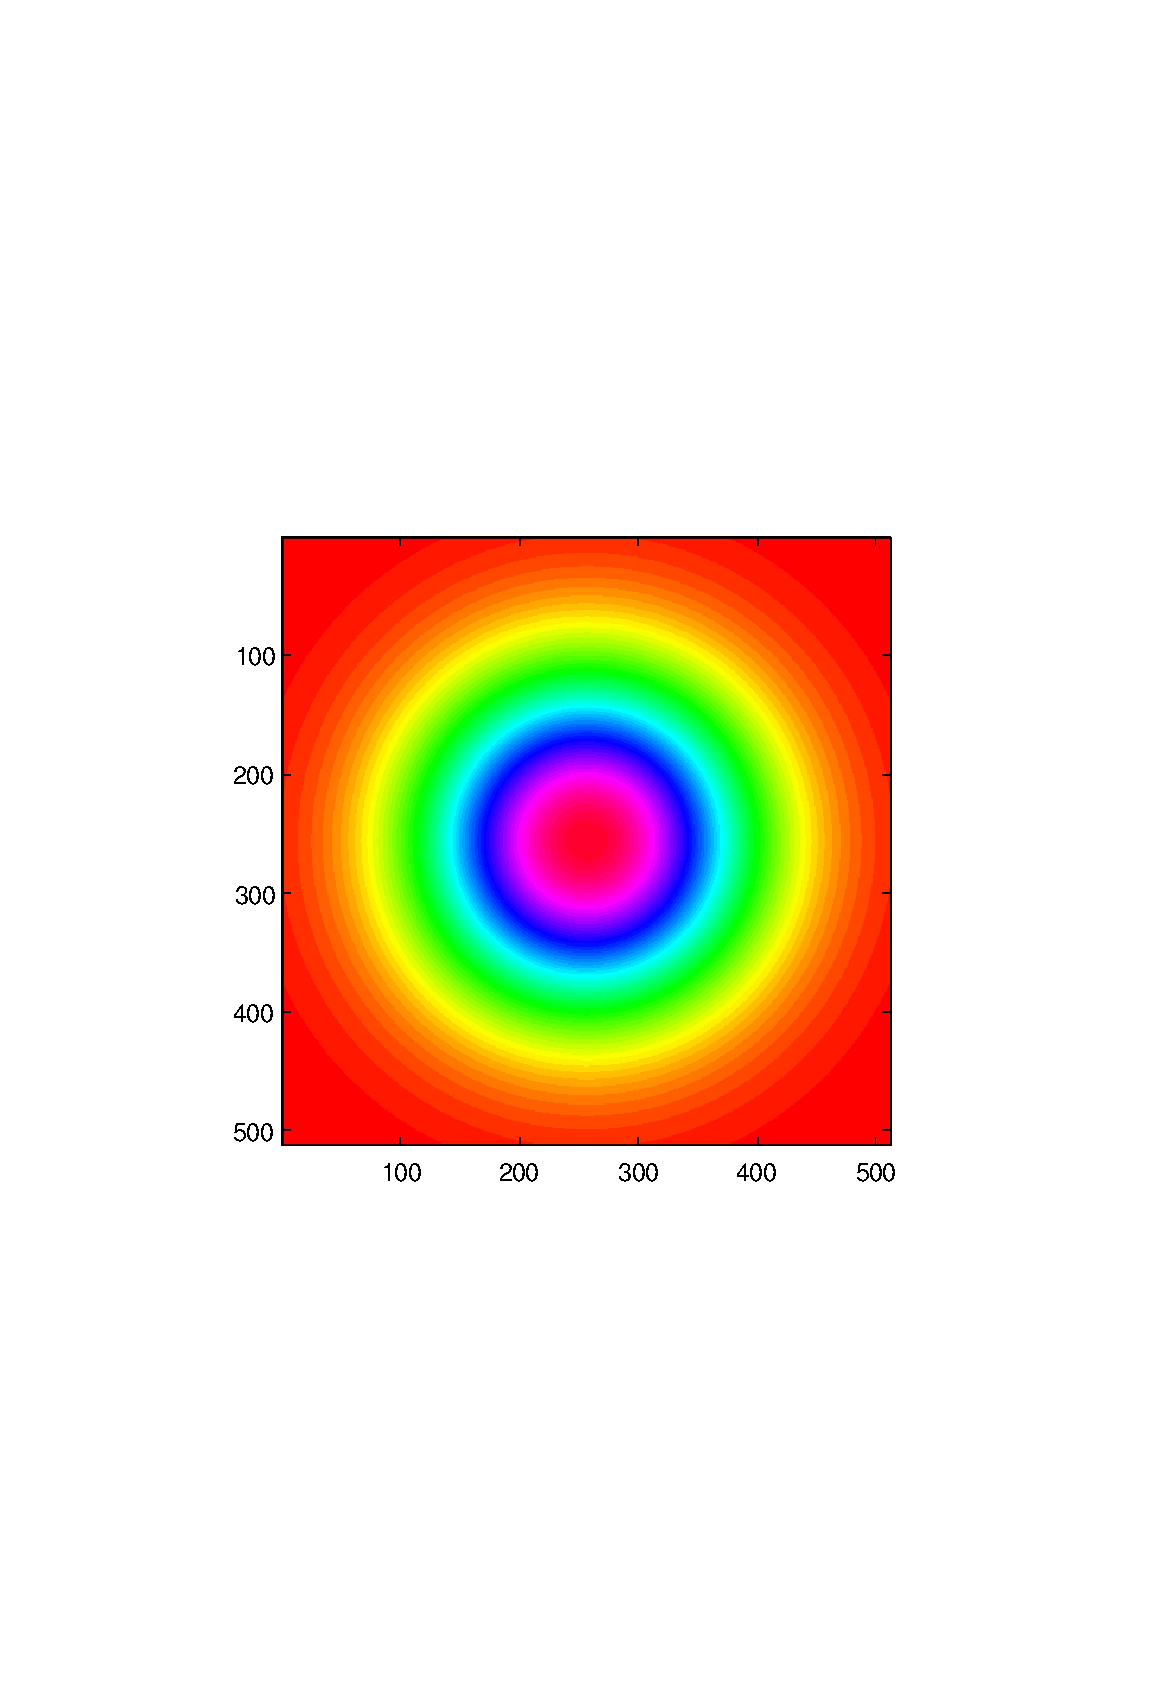
\includegraphics[width=12cm]{colormap1}
\caption{colormap1}
\end{DoxyImage}


Next we switch to the {\ttfamily copper} colormap, and redisplay the image.


\begin{DoxyVerbInclude}
--> colormap(copper);
--> image(Z);
\end{DoxyVerbInclude}


which results in the following image.  
\begin{DoxyImage}
\includegraphics[width=12cm]{colormap2}
\caption{colormap2}
\end{DoxyImage}


If we capture the output of the {\ttfamily copper} command and plot it, we obtain the following result\-:


\begin{DoxyVerbInclude}
--> a = copper;
--> plot(a);
\end{DoxyVerbInclude}


 
\begin{DoxyImage}
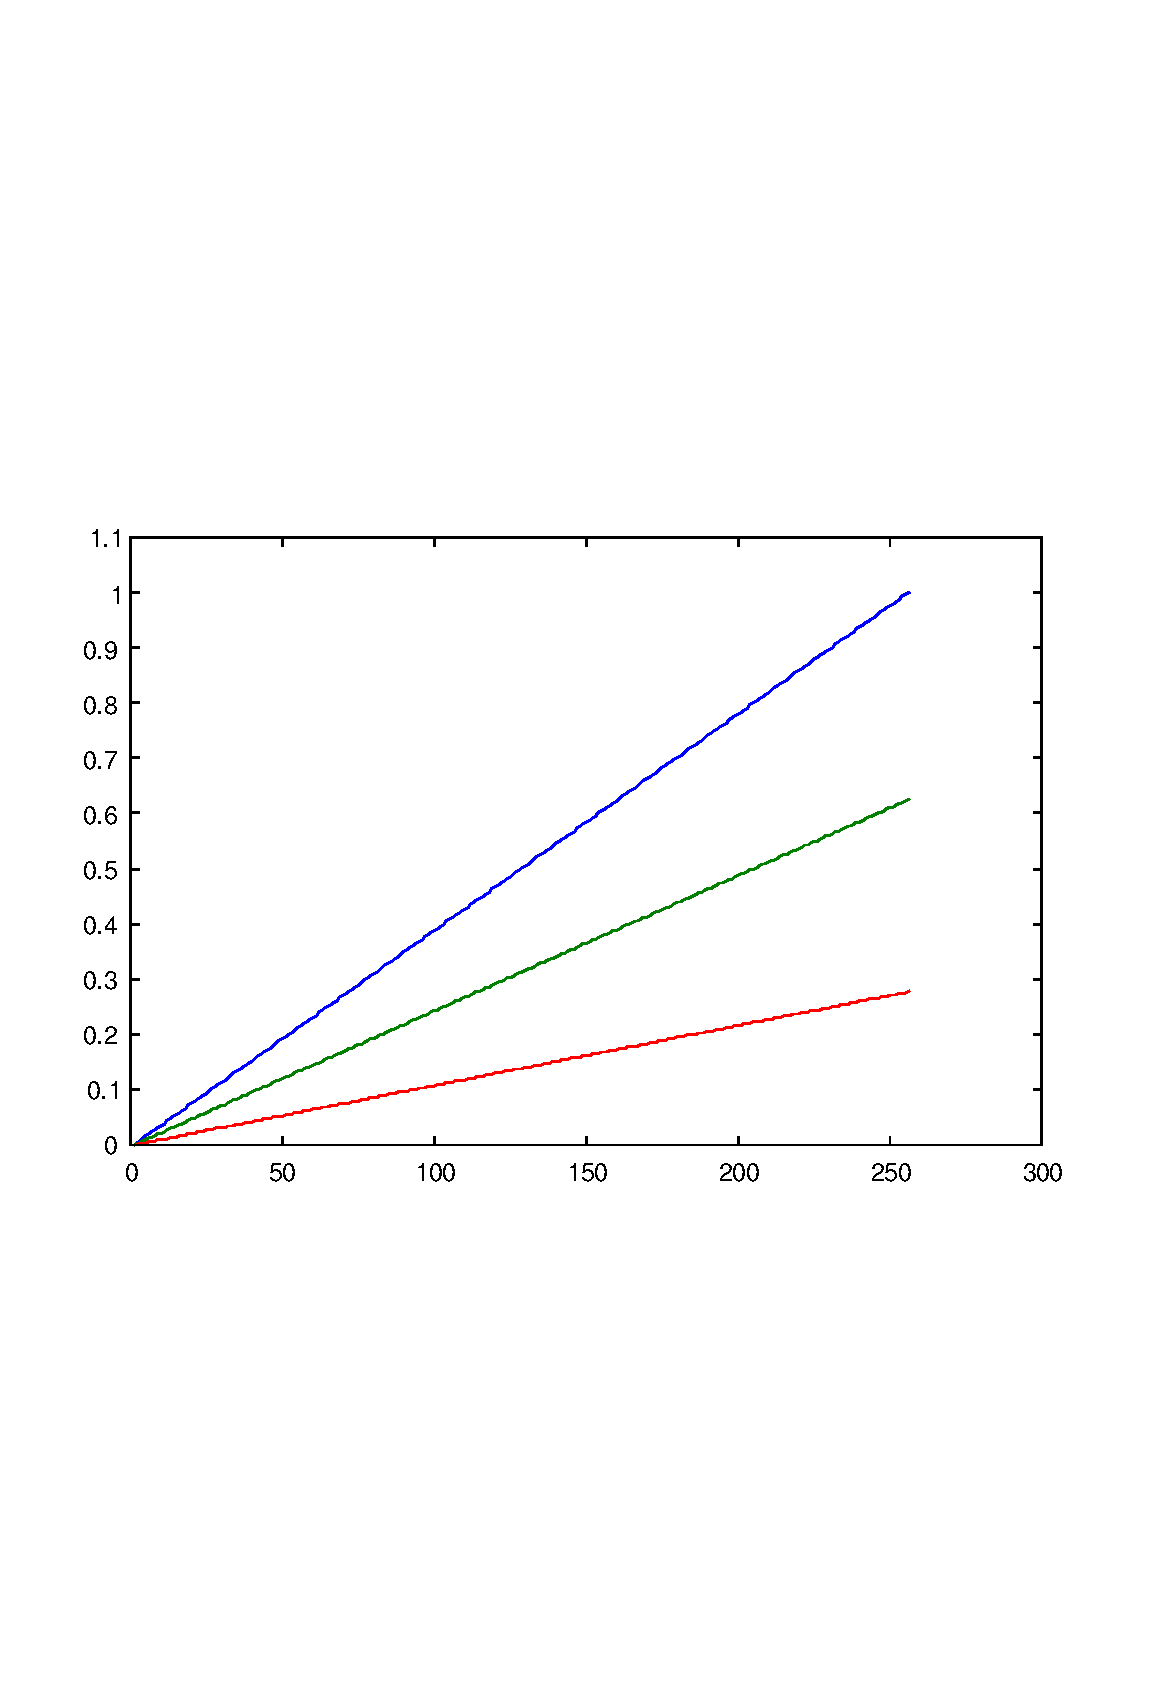
\includegraphics[width=12cm]{colormap3}
\caption{colormap3}
\end{DoxyImage}


Note that in the output that each of the color components are linear functions of the index, with the ratio between the red, blue and green components remaining constant as a function of index. The result is an intensity map with a copper tint. We can similarly construct a colormap of our own by defining the three components seperately. For example, suppose we take three gaussian curves, one for each color, centered on different parts of the index space\-:


\begin{DoxyVerbInclude}
--> t = linspace(0,1,256);
--> A = [exp(-(t-1.0).^2/0.1);exp(-(t-0.5).^2/0.1);exp(-t.^2/0.1)]';
--> plot(A);
\end{DoxyVerbInclude}


 
\begin{DoxyImage}
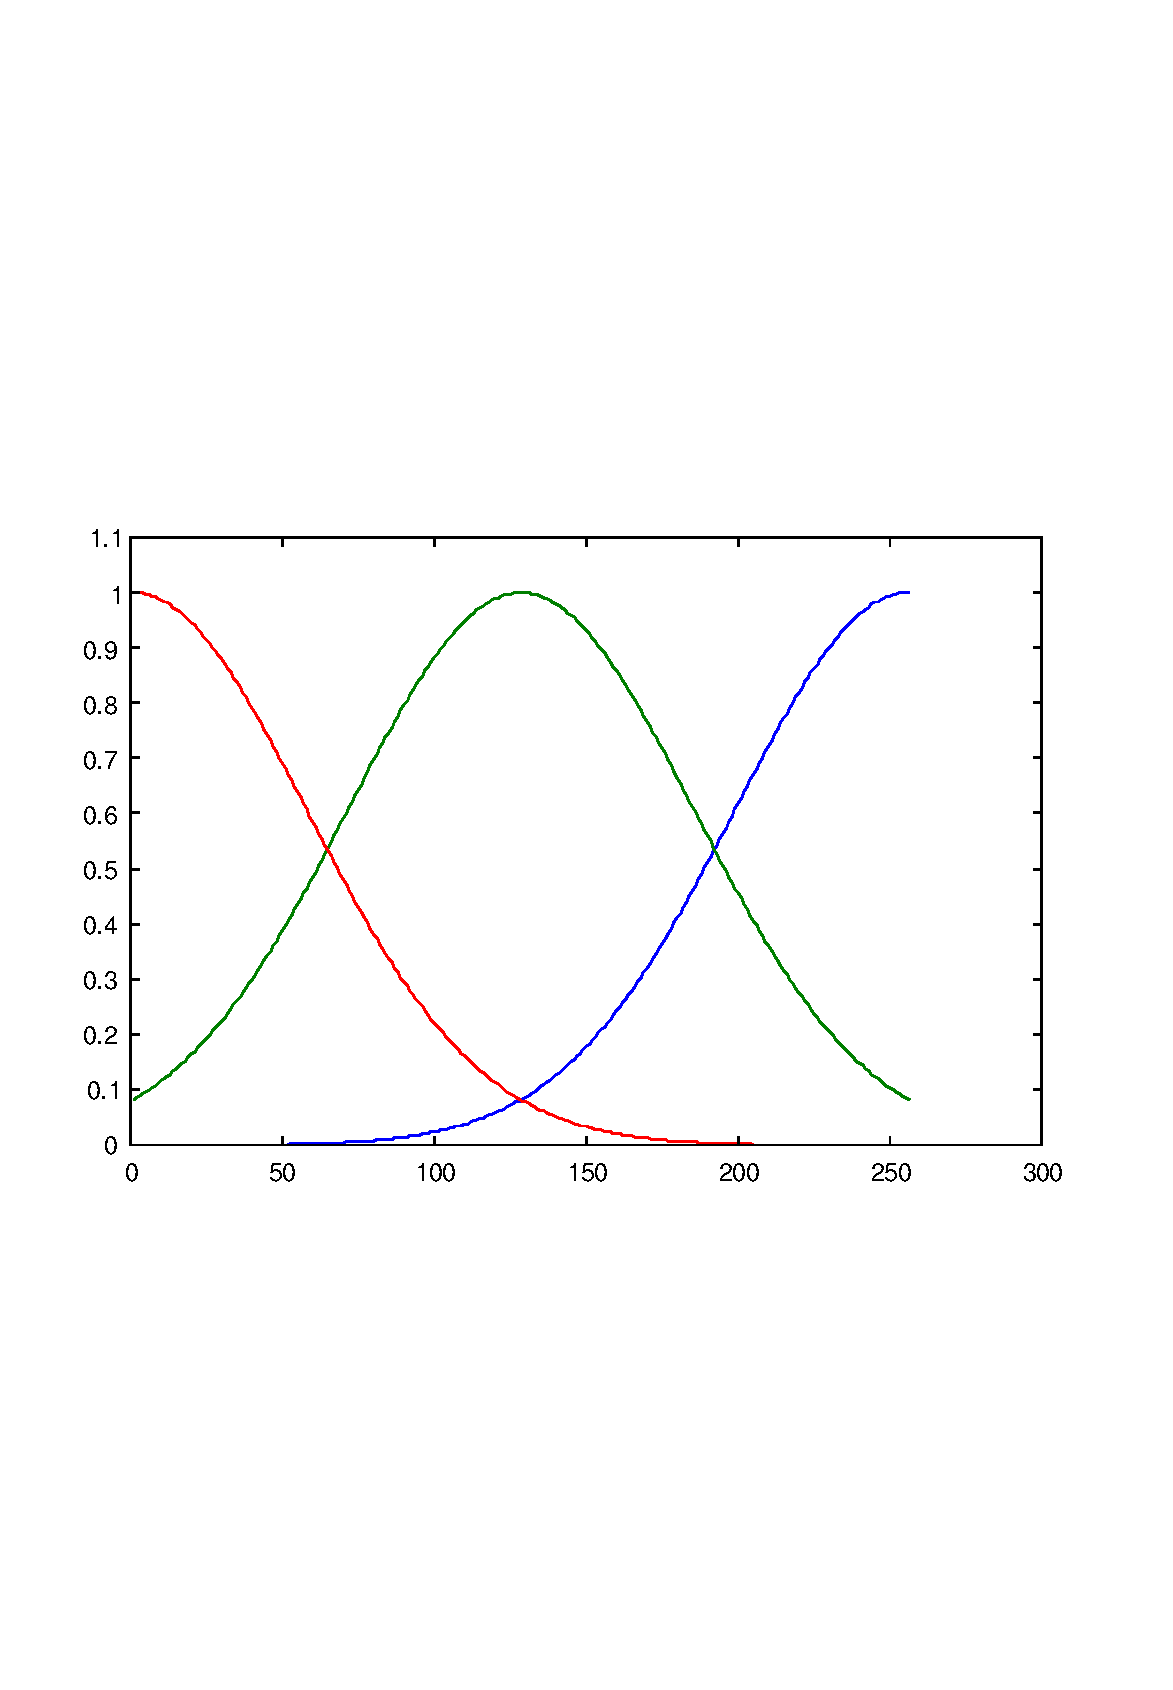
\includegraphics[width=12cm]{colormap4}
\caption{colormap4}
\end{DoxyImage}


The resulting image has dark bands in it near the color transitions.


\begin{DoxyVerbInclude}
--> image(Z);
--> colormap(A);
\end{DoxyVerbInclude}


 
\begin{DoxyImage}
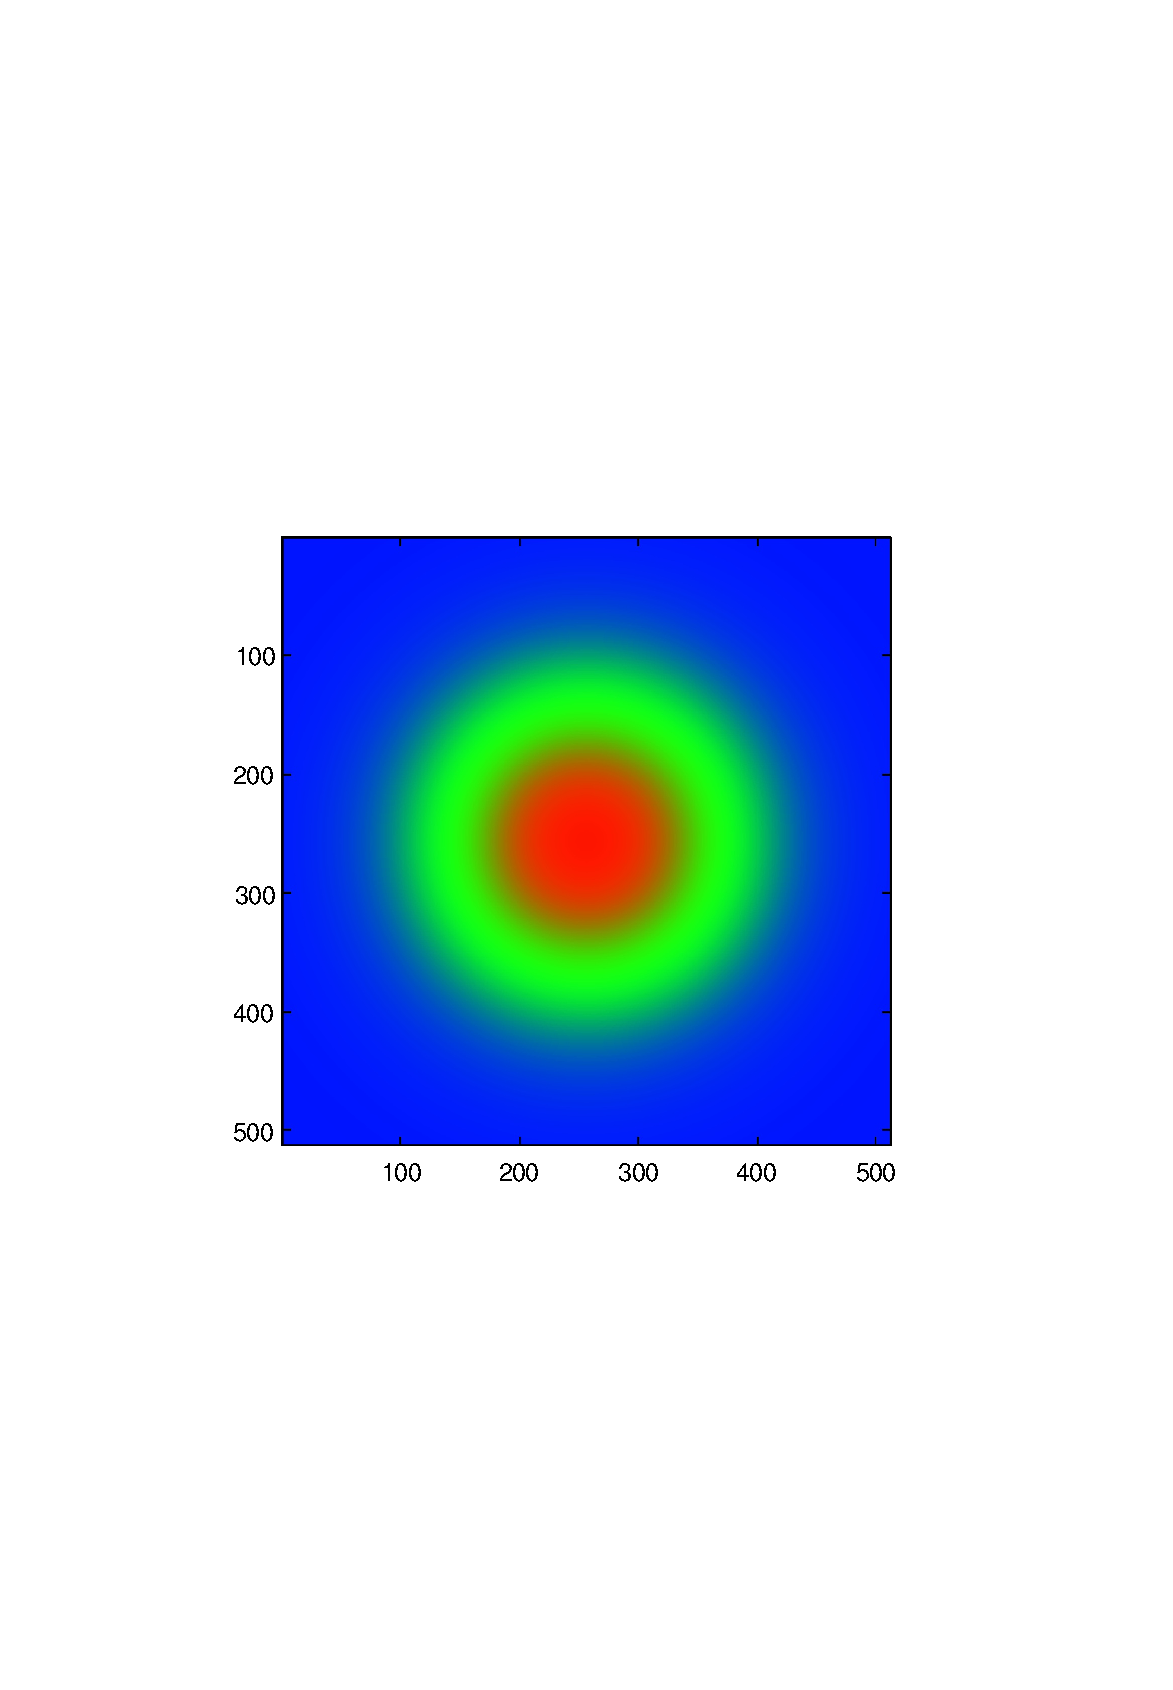
\includegraphics[width=12cm]{colormap5}
\caption{colormap5}
\end{DoxyImage}


These dark bands are a result of the nonuniform color intensity, which we can correct for by renormalizing each color to have the same norm.


\begin{DoxyVerbInclude}
--> w = sqrt(sum(A'.^2));
--> sA = diag(1./w)*A;
--> plot(A);
\end{DoxyVerbInclude}


 
\begin{DoxyImage}
\includegraphics[width=12cm]{colormap6}
\caption{colormap6}
\end{DoxyImage}


The resulting image has no more dark bands.


\begin{DoxyVerbInclude}
--> image(Z);
--> colormap(A);
\end{DoxyVerbInclude}


 
\begin{DoxyImage}
\includegraphics[width=12cm]{colormap7}
\caption{colormap7}
\end{DoxyImage}
 \hypertarget{handle_colorspec}{}\section{C\-O\-L\-O\-R\-S\-P\-E\-C Color Property Description}\label{handle_colorspec}
Section\-: \hyperlink{sec_handle}{Handle-\/\-Based Graphics} \hypertarget{vtkwidgets_vtkxyplotwidget_Usage}{}\subsection{Usage}\label{vtkwidgets_vtkxyplotwidget_Usage}
There are a number of ways of specifying a color value for a color-\/based property. Examples include line colors, marker colors, and the like. One option is to specify color as an R\-G\-B triplet \begin{DoxyVerb}   set(h,'color',[r,g,b])
\end{DoxyVerb}
 where {\ttfamily r,g,b} are between @\mbox{[}0,1\mbox{]} Alternately, you can use color names to specify a color. 
\begin{DoxyItemize}
\item {\ttfamily 'none'} -\/ No color.  
\item {\ttfamily 'y','yellow'} -\/ The color @\mbox{[}1,1,0\mbox{]}@ in R\-G\-B space.  
\item {\ttfamily 'm','magenta'} -\/ The color @\mbox{[}1,0,1\mbox{]}@ in R\-G\-B space.  
\item {\ttfamily 'c','cyan'} -\/ The color @\mbox{[}0,1,1\mbox{]}@ in R\-G\-B space.  
\item {\ttfamily 'r','red'} -\/ The color @\mbox{[}1,0,0\mbox{]}@ in R\-G\-B space.  
\item {\ttfamily 'g','green'} -\/ The color @\mbox{[}0,1,0\mbox{]}@ in R\-G\-B space.  
\item {\ttfamily 'b','blue'} -\/ The color @\mbox{[}0,0,1\mbox{]}@ in R\-G\-B space.  
\item {\ttfamily 'w','white'} -\/ The color @\mbox{[}1,1,1\mbox{]}@ in R\-G\-B space.  
\item {\ttfamily 'k','black'} -\/ The color @\mbox{[}0,0,0\mbox{]}@ in R\-G\-B space.  
\end{DoxyItemize}\hypertarget{handle_contour}{}\section{C\-O\-N\-T\-O\-U\-R Contour Plot Function}\label{handle_contour}
Section\-: \hyperlink{sec_handle}{Handle-\/\-Based Graphics} \hypertarget{vtkwidgets_vtkxyplotwidget_Usage}{}\subsection{Usage}\label{vtkwidgets_vtkxyplotwidget_Usage}
This command generates contour plots. There are several syntaxes for the command. The simplest is \begin{DoxyVerb}  contour(Z)
\end{DoxyVerb}
 which generates a contour plot of the data in matrix {\ttfamily Z}, and will automatically select the contour levels. The {\ttfamily x,y} coordinates of the contour default to {\ttfamily 1\-:n} and {\ttfamily 1\-:m}, where {\ttfamily n} is the number of columns and {\ttfamily m} is the number of rows in the {\ttfamily Z} matrix. Alternately, you can specify a scalar {\ttfamily n} \begin{DoxyVerb}  contour(Z,n)
\end{DoxyVerb}
 which indicates that you want {\ttfamily n} contour levels. For more control, you can provide a vector {\ttfamily v} containing the levels to contour. If you want to generate a contour for a particular level, you must pass a vector {\ttfamily \mbox{[}t,t\mbox{]}} where {\ttfamily t} is the level you want to contour. If you have data that lies on a particular {\ttfamily X,Y} grid, you can pass either vectors {\ttfamily x,y} or matrices {\ttfamily X,Y} to the contour function via \begin{DoxyVerb}  contour(X,Y,Z)
  contour(X,Y,Z,n)
  contour(X,Y,Z,v)
\end{DoxyVerb}
 Each form of {\ttfamily contour} can optionally take a line spec to indicate the color and linestyle of the contours to draw\-: \begin{DoxyVerb}  contour(...,linespec)
\end{DoxyVerb}
 or any of the other forms of {\ttfamily contour}. Furthermore, you can supply an axis to target the {\ttfamily contour} plot to (so that it does not get added to the current axis, which is the default)\-: \begin{DoxyVerb}  contour(axis_handle,...)
\end{DoxyVerb}
 Finally, the {\ttfamily contour} command returns a handle to the newly returned contour plot. \begin{DoxyVerb}  handle = contour(...)
\end{DoxyVerb}
 To place labels on the contour plot, use the {\ttfamily clabel} function. \hypertarget{variables_struct_Example}{}\subsection{Example}\label{variables_struct_Example}
Here is a simple example of a contour plot with the default {\ttfamily x,y} coordinates\-:


\begin{DoxyVerbInclude}
--> [x,y] = meshgrid(linspace(-1,1,25),linspace(-2,2,30));
--> z = x.*exp(-x.^2-y.^2);
--> contour(z)
\end{DoxyVerbInclude}


which results in the following plot  
\begin{DoxyImage}
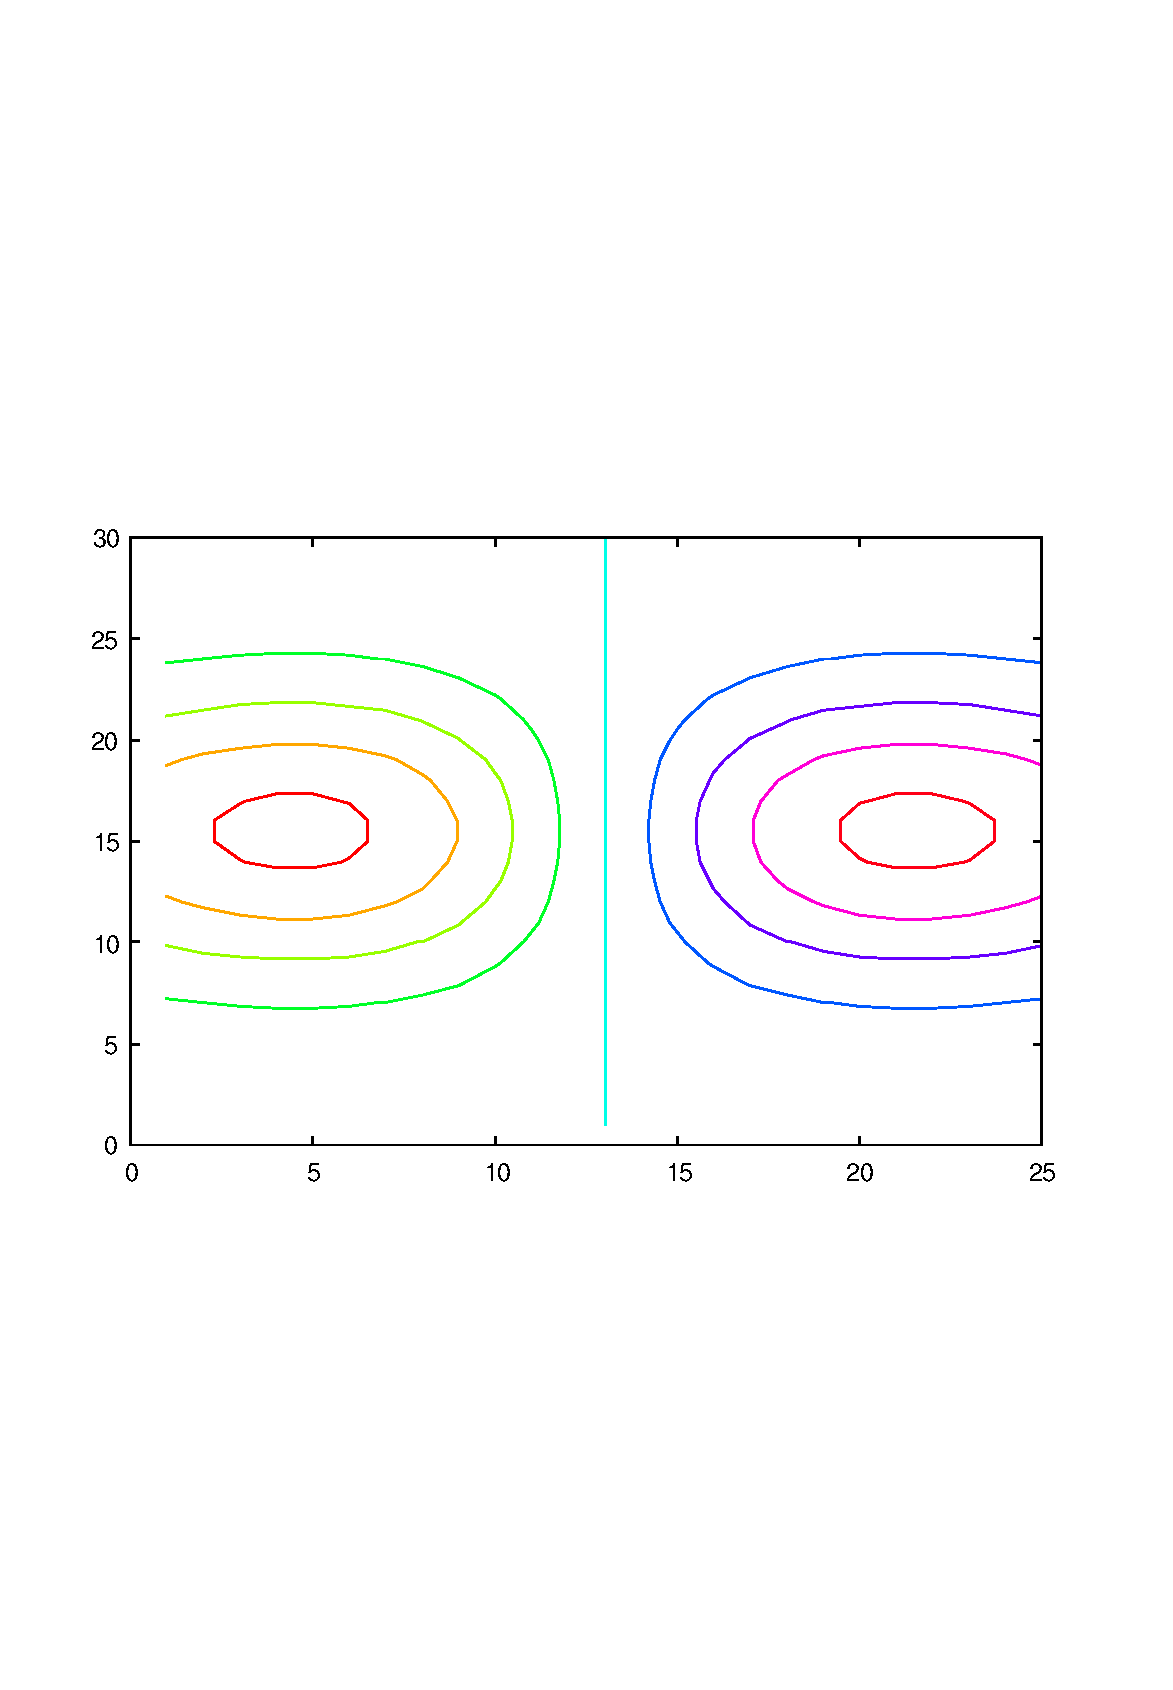
\includegraphics[width=12cm]{contour1}
\caption{contour1}
\end{DoxyImage}
 Here, we specify the {\ttfamily x} and {\ttfamily y} coordinates explictly


\begin{DoxyVerbInclude}
--> contour(x,y,z)
\end{DoxyVerbInclude}


note that the axis limits have changed appropriately  
\begin{DoxyImage}
\includegraphics[width=12cm]{contour2}
\caption{contour2}
\end{DoxyImage}
 By default, contours are created at values selected by Free\-Mat. To provide our own set of contour values (asymmetrically about zero in this case), we supply them as


\begin{DoxyVerbInclude}
--> contour(x,y,z,[-.4,0.,3])
\end{DoxyVerbInclude}


which is here  
\begin{DoxyImage}
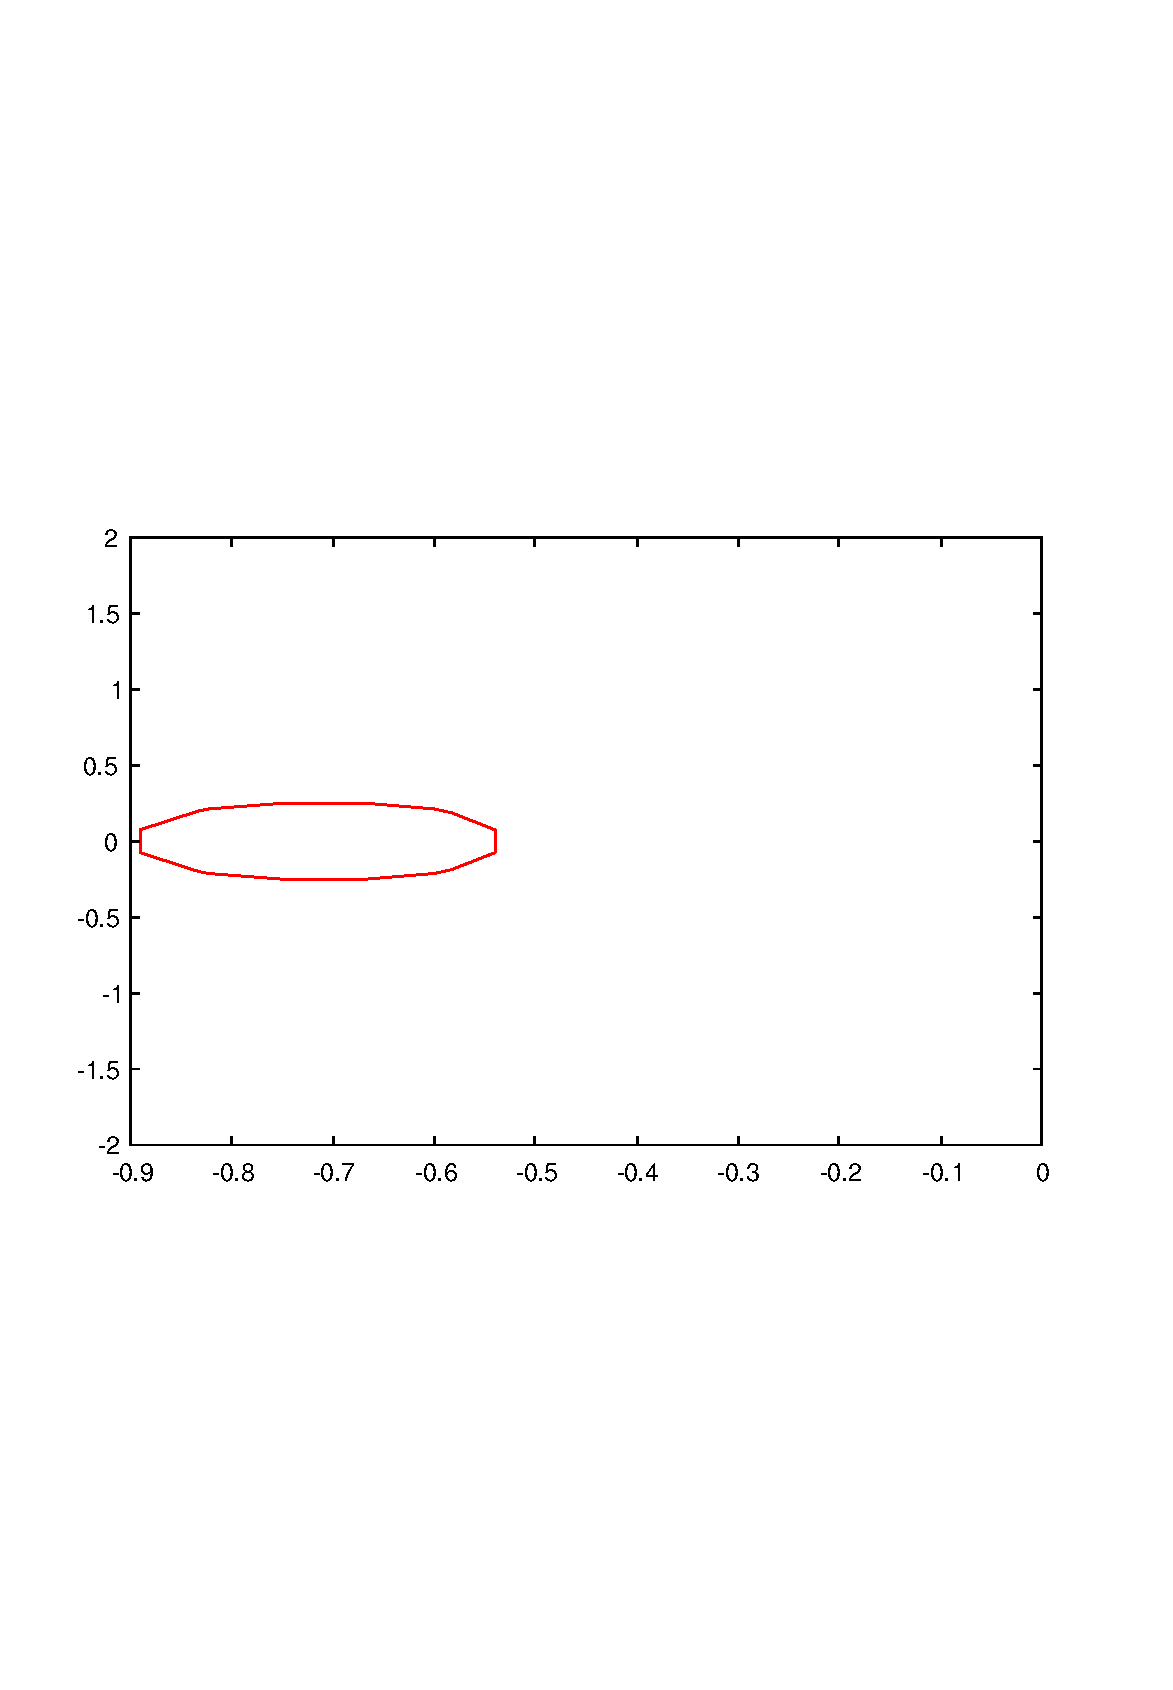
\includegraphics[width=12cm]{contour3}
\caption{contour3}
\end{DoxyImage}
 Also be default, {\ttfamily contour} uses the current color map and {\ttfamily clim} limits to determine the coloring of the contours. Here, we override the color spec so that we have all black contour


\begin{DoxyVerbInclude}
--> contour(x,y,z,'b-')
\end{DoxyVerbInclude}


which is here  
\begin{DoxyImage}
\includegraphics[width=12cm]{contour4}
\caption{contour4}
\end{DoxyImage}
 \hypertarget{handle_contour3}{}\section{C\-O\-N\-T\-O\-U\-R3 3\-D Contour Plot Function}\label{handle_contour3}
Section\-: \hyperlink{sec_handle}{Handle-\/\-Based Graphics} \hypertarget{vtkwidgets_vtkxyplotwidget_Usage}{}\subsection{Usage}\label{vtkwidgets_vtkxyplotwidget_Usage}
This command generates contour plots where the lines are plotted in 3\-D. The syntax for its use is identical to the {\ttfamily contour} function. Please see its help for details. \hypertarget{variables_struct_Example}{}\subsection{Example}\label{variables_struct_Example}
Here is a simple example of a 3\-D contour plot.


\begin{DoxyVerbInclude}
--> [x,y] = meshgrid([-2:.25:2]);
--> z=x.*exp(-x.^2-y.^2);
--> contour3(x,y,z,30);
--> axis square;
--> view(-15,25)
\end{DoxyVerbInclude}


The resulting plot  
\begin{DoxyImage}
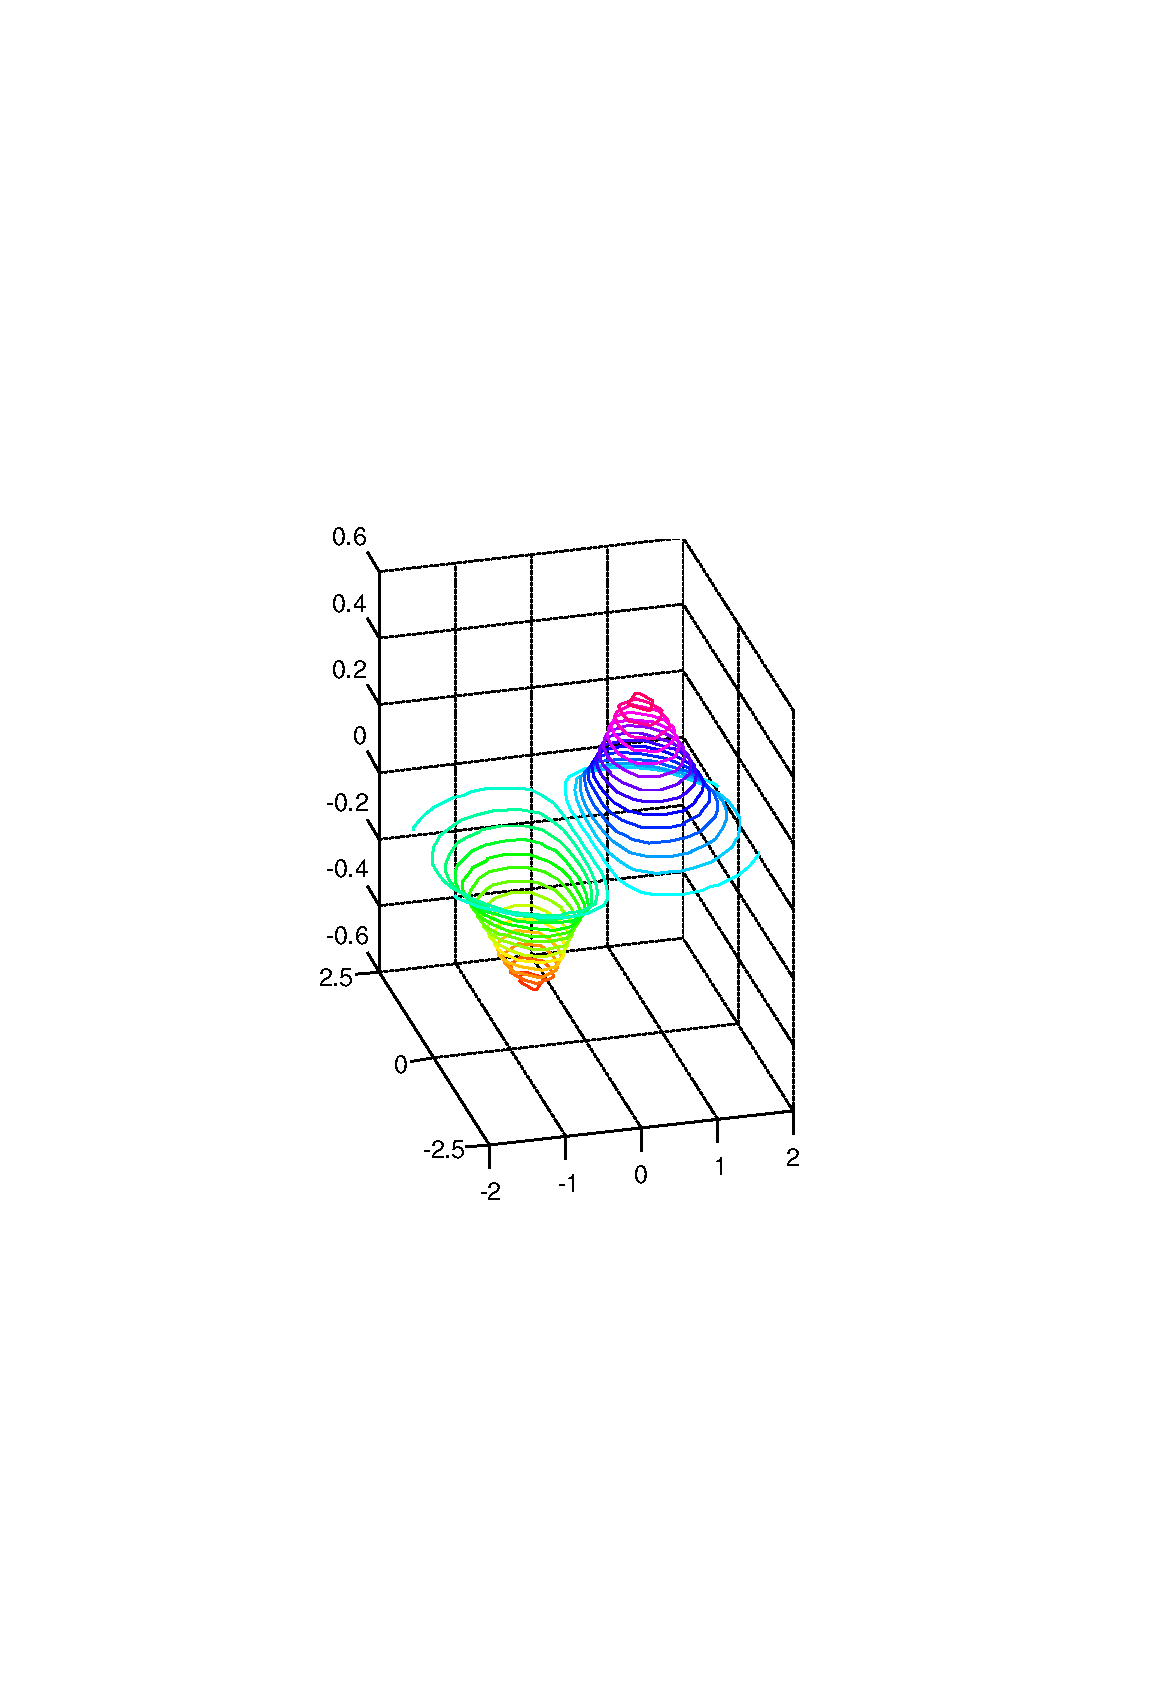
\includegraphics[width=12cm]{contour3_1}
\caption{contour3\-\_\-1}
\end{DoxyImage}
 \hypertarget{handle_copper}{}\section{C\-O\-P\-P\-E\-R Copper Colormap}\label{handle_copper}
Section\-: \hyperlink{sec_handle}{Handle-\/\-Based Graphics} \hypertarget{vtkwidgets_vtkxyplotwidget_Usage}{}\subsection{Usage}\label{vtkwidgets_vtkxyplotwidget_Usage}
Returns a copper colormap. The syntax for its use is \begin{DoxyVerb}   y = copper
\end{DoxyVerb}
 \hypertarget{variables_struct_Example}{}\subsection{Example}\label{variables_struct_Example}
Here is an example of an image displayed with the {\ttfamily copper} colormap


\begin{DoxyVerbInclude}
--> x = linspace(-1,1,512)'*ones(1,512);
--> y = x';
--> Z = exp(-(x.^2+y.^2)/0.3);
--> image(Z);
--> colormap(copper);
\end{DoxyVerbInclude}


which results in the following image  
\begin{DoxyImage}
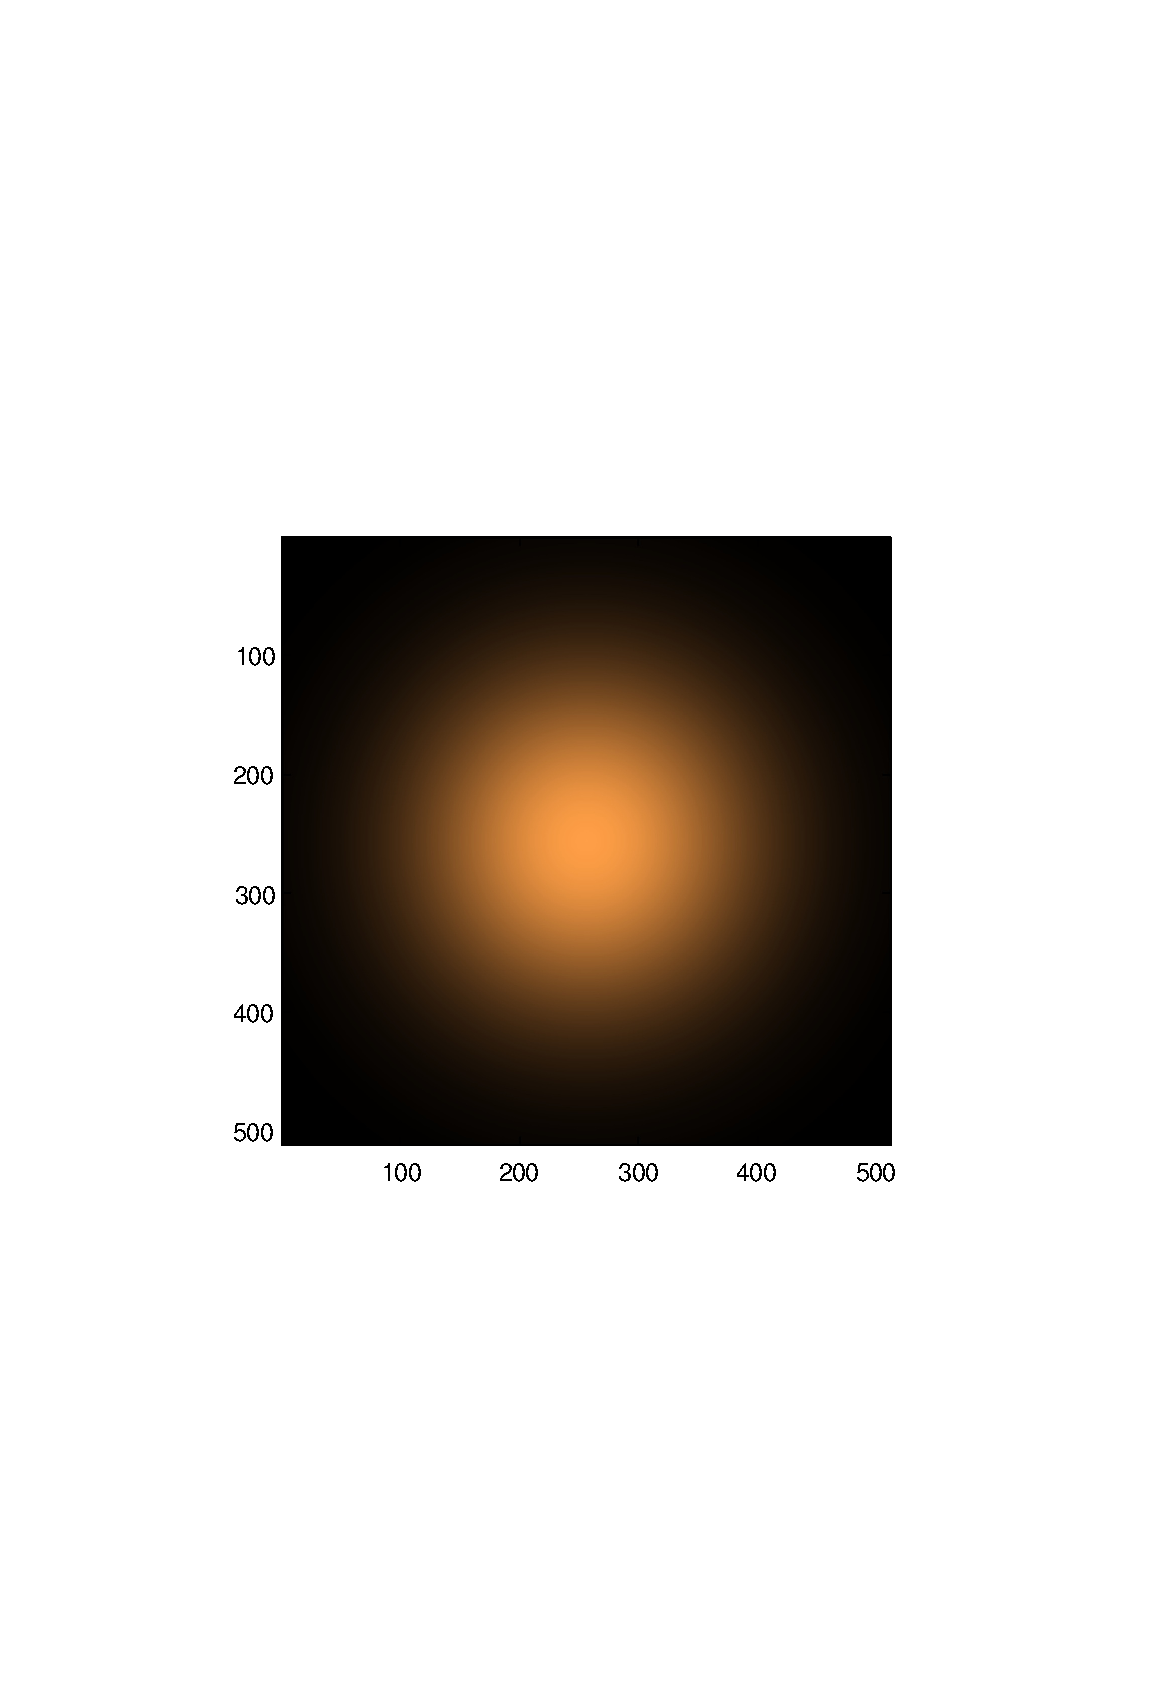
\includegraphics[width=12cm]{copper1}
\caption{copper1}
\end{DoxyImage}
 \hypertarget{handle_copy}{}\section{C\-O\-P\-Y Copy Figure Window}\label{handle_copy}
Section\-: \hyperlink{sec_handle}{Handle-\/\-Based Graphics} \hypertarget{vtkwidgets_vtkxyplotwidget_Usage}{}\subsection{Usage}\label{vtkwidgets_vtkxyplotwidget_Usage}
Copies the currently active figure window to the clipboard. The syntax for its use is\-: \begin{DoxyVerb}   copy
\end{DoxyVerb}
 The resulting figure is copied as a bitmap to the clipboard, and can then be pasted into any suitable application. \hypertarget{handle_countour}{}\section{C\-O\-U\-N\-T\-O\-U\-R Contour Object Properties}\label{handle_countour}
Section\-: \hyperlink{sec_handle}{Handle-\/\-Based Graphics} \hypertarget{vtkwidgets_vtkxyplotwidget_Usage}{}\subsection{Usage}\label{vtkwidgets_vtkxyplotwidget_Usage}
Below is a summary of the properties for a line series. 
\begin{DoxyItemize}
\item {\ttfamily contourmatrix} -\/ {\ttfamily array} -\/ the matrix containing contour data for the plot. This is a {\ttfamily 2 x N} matrix containing x and y coordinates for points on the contours. In addition, each contour line starts with a column containing the number of points and the contour value.  
\item {\ttfamily displayname} -\/ {\ttfamily string} -\/ The name of this line series as it appears in a legend.  
\item {\ttfamily floating} -\/ {\ttfamily \{'on','off'\}} -\/ set to on to have floating (3\-D) contours  
\item {\ttfamily levellist} -\/ {\ttfamily vector} -\/ a vector of Z-\/values for the contours  
\item {\ttfamily levellistmode} -\/ {\ttfamily \{'auto','manual'\}} -\/ set to auto for automatic selection of Z-\/values of the contours.  
\item {\ttfamily linecolor} -\/ color of the contour lines.  
\item {\ttfamily linestyle} -\/ {\ttfamily \{'-\/','--','\-:','-\/.','none'\}} -\/ the line style to draw the contour in.  
\item {\ttfamily linewidth} -\/ {\ttfamily scalar} -\/ the width of the lines  
\item {\ttfamily parent} -\/ {\ttfamily handle} -\/ The axis that contains this object  
\item {\ttfamily tag} -\/ {\ttfamily string} -\/ A string that can be used to tag the object.  
\item {\ttfamily type} -\/ {\ttfamily string} -\/ Returns the string {\ttfamily 'contour'}.  
\item {\ttfamily userdata} -\/ {\ttfamily array} -\/ Available to store any variable you want in the handle object.  
\item {\ttfamily visible} -\/ {\ttfamily \{'on','off'\}} -\/ Controls visibility of the the line.  
\item {\ttfamily xdata} -\/ {\ttfamily matrix} -\/ Contains the x coordinates of the surface on which the zdata is defined. This can either be a monotonic vector of the same number of columns as {\ttfamily zdata}, or a 2\-D matrix that is the same size as {\ttfamily zdata}.  
\item {\ttfamily xdatamode} -\/ {\ttfamily \{'auto','manual'\}} -\/ When set to {\ttfamily 'auto'} Free\-Mat will autogenerate the x coordinates for the contours. These values will be {\ttfamily 1,..,N} where {\ttfamily N} is the number of columns of {\ttfamily zdata}.  
\item {\ttfamily ydata} -\/ {\ttfamily matrix} -\/ Contains the y coordinates of the surface on which the zdata is defined. This can either be a monotonic vector of the same number of rows as {\ttfamily zdata} or a 2\-D matrix that is the same size as {\ttfamily zdata}.  
\item {\ttfamily ydatamode} -\/ {\ttfamily \{'auto','manual'\}} -\/ When set to {\ttfamily 'auto'} Free\-Mat will autogenerate the y coordinates for the contour data.  
\item {\ttfamily zdata} -\/ {\ttfamily matrix} -\/ The matrix of z values that are to be contoured.  
\end{DoxyItemize}\hypertarget{handle_datacursormode}{}\section{D\-A\-T\-A\-C\-U\-R\-S\-O\-R\-M\-O\-D\-E Interactive Data Cursor}\label{handle_datacursormode}
Section\-: \hyperlink{sec_handle}{Handle-\/\-Based Graphics} \hypertarget{vtkwidgets_vtkxyplotwidget_Usage}{}\subsection{Usage}\label{vtkwidgets_vtkxyplotwidget_Usage}
Toggles the data cursor which allows interactive data exploration. \begin{DoxyVerb}   datacursormode('on')
\end{DoxyVerb}
 \hypertarget{handle_drawnow}{}\section{D\-R\-A\-W\-N\-O\-W Flush the Event Queue}\label{handle_drawnow}
Section\-: \hyperlink{sec_handle}{Handle-\/\-Based Graphics} \hypertarget{vtkwidgets_vtkxyplotwidget_Usage}{}\subsection{Usage}\label{vtkwidgets_vtkxyplotwidget_Usage}
The {\ttfamily drawnow} function can be used to process the events in the event queue of the Free\-Mat application. The syntax for its use is \begin{DoxyVerb}   drawnow
\end{DoxyVerb}
 Now that Free\-Mat is threaded, you do not generally need to call this function, but it is provided for compatibility. \hypertarget{handle_figlower}{}\section{F\-I\-G\-L\-O\-W\-E\-R Lower a Figure Window}\label{handle_figlower}
Section\-: \hyperlink{sec_handle}{Handle-\/\-Based Graphics} \hypertarget{vtkwidgets_vtkxyplotwidget_Usage}{}\subsection{Usage}\label{vtkwidgets_vtkxyplotwidget_Usage}
Lowers a figure window indicated by the figure number. The syntax for its use is \begin{DoxyVerb}  figlower(fignum)
\end{DoxyVerb}
 where {\ttfamily fignum} is the number of the figure to lower. The figure will be lowerd to the bottom of the G\-U\-I stack (meaning that it we be behind other windows). Note that this function does not cause {\ttfamily fignum} to become the current figure, you must use the {\ttfamily figure} command for that. Similarly, if {\ttfamily fignum} is the current figure, it will remain the current figure (even though the figure is now behind others). \hypertarget{handle_figraise}{}\section{F\-I\-G\-R\-A\-I\-S\-E Raise a Figure Window}\label{handle_figraise}
Section\-: \hyperlink{sec_handle}{Handle-\/\-Based Graphics} \hypertarget{vtkwidgets_vtkxyplotwidget_Usage}{}\subsection{Usage}\label{vtkwidgets_vtkxyplotwidget_Usage}
Raises a figure window indicated by the figure number. The syntax for its use is \begin{DoxyVerb}  figraise(fignum)
\end{DoxyVerb}
 where {\ttfamily fignum} is the number of the figure to raise. The figure will be raised to the top of the G\-U\-I stack (meaning that it we be visible). Note that this function does not cause {\ttfamily fignum} to become the current figure, you must use the {\ttfamily figure} command for that. \hypertarget{handle_figure}{}\section{F\-I\-G\-U\-R\-E Figure Window Select and Create Function}\label{handle_figure}
Section\-: \hyperlink{sec_handle}{Handle-\/\-Based Graphics} \hypertarget{vtkwidgets_vtkxyplotwidget_Usage}{}\subsection{Usage}\label{vtkwidgets_vtkxyplotwidget_Usage}
Changes the active figure window to the specified figure number. The general syntax for its use is \begin{DoxyVerb}  figure(number)
\end{DoxyVerb}
 where {\ttfamily number} is the figure number to use. If the figure window corresponding to {\ttfamily number} does not already exist, a new window with this number is created. If it does exist then it is brought to the forefront and made active. You can use {\ttfamily gcf} to obtain the number of the current figure.

Note that the figure number is also the handle for the figure. While for most graphical objects (e.\-g., axes, lines, images), the handles are large integers, for figures, the handle is the same as the figure number. This means that the figure number can be passed to {\ttfamily set} and {\ttfamily get} to modify the properties of the current figure, (e.\-g., the colormap). So, for figure {\ttfamily 3}, for example, you can use {\ttfamily get(3,'colormap')} to retrieve the colormap for the current figure. \hypertarget{handle_figureproperties}{}\section{F\-I\-G\-U\-R\-E\-P\-R\-O\-P\-E\-R\-T\-I\-E\-S Figure Object Properties}\label{handle_figureproperties}
Section\-: \hyperlink{sec_handle}{Handle-\/\-Based Graphics} \hypertarget{vtkwidgets_vtkxyplotwidget_Usage}{}\subsection{Usage}\label{vtkwidgets_vtkxyplotwidget_Usage}
Below is a summary of the properties for the axis. 
\begin{DoxyItemize}
\item {\ttfamily alphamap} -\/ {\ttfamily vector} -\/ Contains the alpha (transparency) map for the figure. If this is set to a scalar, then all values are mapped to the same transparency. It defaults to {\ttfamily 1}, which is all values being fully opaque. If you set this to a vector, the values of graphics objects will be mapped to different transparency values, based on the setting of their {\ttfamily alphadatamapping} property.  
\item {\ttfamily color} -\/ {\ttfamily colorspec} -\/ The background color of the figure (defaults to a gray {\ttfamily \mbox{[}0.\-6,0.\-6,0.\-6\mbox{]}}). During printing, this color is set to white, and then is restored.  
\item {\ttfamily colormap} -\/ {\ttfamily color vector} -\/ an {\ttfamily N x 3} matrix of R\-G\-B values that specifies the colormap for the figure. Defaults to an {\ttfamily H\-S\-V} map.  
\item {\ttfamily children} -\/ {\ttfamily handle vector} -\/ the handles for objects that are children of this figure. These should be axis objects.  
\item {\ttfamily currentaxes} -\/ {\ttfamily handle} -\/ the handle for the current axes. Also returned by {\ttfamily gca}.  
\item {\ttfamily doublebuffer} -\/ Not used.  
\item {\ttfamily parent} -\/ Not used.  
\item {\ttfamily position} -\/ Not used.  
\item {\ttfamily type} -\/ {\ttfamily string} -\/ returns the string {\ttfamily 'figure'}.  
\item {\ttfamily userdata} -\/ {\ttfamily array} -\/ arbitrary array you can use to store data associated with the figure.  
\item {\ttfamily nextplot} -\/ {\ttfamily \{'add','replace','replacechildren'\}} -\/ If set to {\ttfamily 'add'} then additional axes are added to the list of children for the current figure. If set to {\ttfamily 'replace'}, then a new axis replaces all of the existing children.  
\item {\ttfamily figsize} -\/ {\ttfamily two vector} -\/ the size of the figure window in pixels (width x height).  
\item {\ttfamily renderer} -\/ {\ttfamily \{'painters','opengl'\}} -\/ When set to {\ttfamily 'painters'} drawing is based on the Qt drawing methods (which can handle flat shading of surfaces with transparency). If you set the renderer to {\ttfamily 'opengl'} then Open\-G\-L is used for rendering. Support for Open\-G\-L is currently in the alpha stage, and Free\-Mat does not enable it automatically. You can set the renderer mode to {\ttfamily 'opengl'} manually to experiment. Also, Open\-G\-L figures cannot be printed yet.  
\end{DoxyItemize}\hypertarget{handle_gca}{}\section{G\-C\-A Get Current Axis}\label{handle_gca}
Section\-: \hyperlink{sec_handle}{Handle-\/\-Based Graphics} \hypertarget{vtkwidgets_vtkxyplotwidget_Usage}{}\subsection{Usage}\label{vtkwidgets_vtkxyplotwidget_Usage}
Returns the handle for the current axis. The syntax for its use is \begin{DoxyVerb}  handle = gca
\end{DoxyVerb}
 where {\ttfamily handle} is the handle of the active axis. All object creation functions will be children of this axis. \hypertarget{handle_gcf}{}\section{G\-C\-F Get Current Figure}\label{handle_gcf}
Section\-: \hyperlink{sec_handle}{Handle-\/\-Based Graphics} \hypertarget{vtkwidgets_vtkxyplotwidget_Usage}{}\subsection{Usage}\label{vtkwidgets_vtkxyplotwidget_Usage}
Returns the figure number for the current figure (which is also its handle, and can be used to set properties of the current figure using {\ttfamily set}). The syntax for its use is \begin{DoxyVerb}  figure_number = gcf
\end{DoxyVerb}
 where {\ttfamily figure\-\_\-number} is the number of the active figure (also the handle of the figure).

Note that figures have handles, just like axes, images, plots, etc. However the handles for figures match the figure number (while handles for other graphics objects tend to be large, somewhat arbitrary integers). So, to retrieve the colormap of the current figure, you could use {\ttfamily get(gcf,'colormap')}, or to obtain the colormap for figure 3, use {\ttfamily get(3,'colormap')}. \hypertarget{handle_get}{}\section{G\-E\-T Get Object Property}\label{handle_get}
Section\-: \hyperlink{sec_handle}{Handle-\/\-Based Graphics} \hypertarget{vtkwidgets_vtkxyplotwidget_Usage}{}\subsection{Usage}\label{vtkwidgets_vtkxyplotwidget_Usage}
This function allows you to retrieve the value associated with a property. The syntax for its use is \begin{DoxyVerb}  value = get(handle,property)
\end{DoxyVerb}
 where {\ttfamily property} is a string containing the name of the property, and {\ttfamily value} is the value for that property. The type of the variable {\ttfamily value} depends on the property being set. See the help for the properties to see what values you can set. \hypertarget{handle_glshow}{}\section{G\-L\-S\-H\-O\-W Show a G\-L Assembly in a G\-L Window}\label{handle_glshow}
Section\-: \hyperlink{sec_handle}{Handle-\/\-Based Graphics} \hypertarget{vtkwidgets_vtkxyplotwidget_Usage}{}\subsection{Usage}\label{vtkwidgets_vtkxyplotwidget_Usage}
Shows a G\-L Assembly in a G\-L Window. The syntax for its use is \begin{DoxyVerb}  glshow(name,scale)
\end{DoxyVerb}
 which shows the {\ttfamily glassembly} named {\ttfamily name} in a new G\-L window, with the scale set to {\ttfamily scale}. Roughly speaking {\ttfamily scale} should represent the radial size of the object that you want to see in the window. \hypertarget{handle_gray}{}\section{G\-R\-A\-Y Gray Colormap}\label{handle_gray}
Section\-: \hyperlink{sec_handle}{Handle-\/\-Based Graphics} \hypertarget{vtkwidgets_vtkxyplotwidget_Usage}{}\subsection{Usage}\label{vtkwidgets_vtkxyplotwidget_Usage}
Returns a gray colormap. The syntax for its use is \begin{DoxyVerb}   y = gray
\end{DoxyVerb}
 \hypertarget{variables_struct_Example}{}\subsection{Example}\label{variables_struct_Example}
Here is an example of an image displayed with the {\ttfamily gray} colormap


\begin{DoxyVerbInclude}
--> x = linspace(-1,1,512)'*ones(1,512);
--> y = x';
--> Z = exp(-(x.^2+y.^2)/0.3);
--> image(Z);
--> colormap(gray);
\end{DoxyVerbInclude}


which results in the following image  
\begin{DoxyImage}
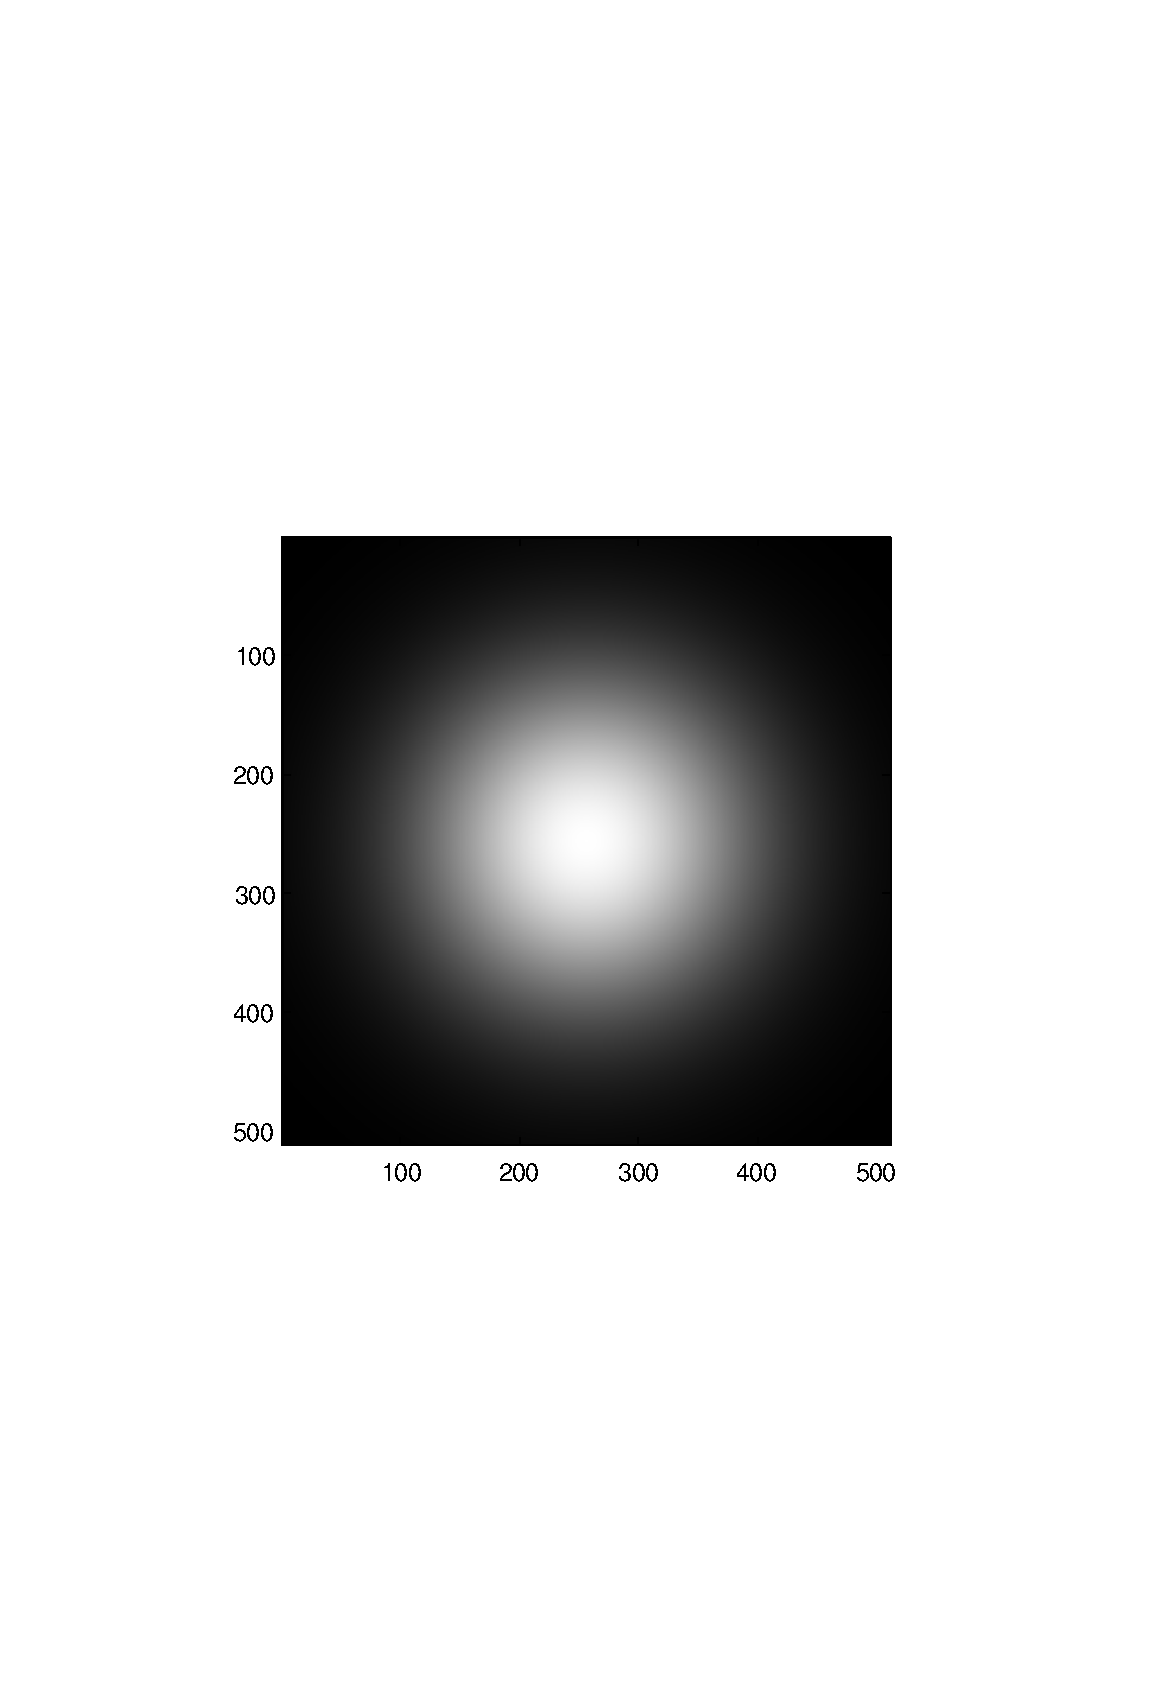
\includegraphics[width=12cm]{gray1}
\caption{gray1}
\end{DoxyImage}
 \hypertarget{handle_grid}{}\section{G\-R\-I\-D Plot Grid Toggle Function}\label{handle_grid}
Section\-: \hyperlink{sec_handle}{Handle-\/\-Based Graphics} \hypertarget{vtkwidgets_vtkxyplotwidget_Usage}{}\subsection{Usage}\label{vtkwidgets_vtkxyplotwidget_Usage}
Toggles the drawing of grid lines on the currently active plot. The general syntax for its use is \begin{DoxyVerb}   grid(state)
\end{DoxyVerb}
 where {\ttfamily state} is either \begin{DoxyVerb}   grid('on')
\end{DoxyVerb}
 to activate the grid lines, or \begin{DoxyVerb}   grid('off')
\end{DoxyVerb}
 to deactivate the grid lines. If you specify no argument then {\ttfamily grid} toggles the state of the grid\-: \begin{DoxyVerb}   grid
\end{DoxyVerb}
 You can also specify a particular axis to the grid command \begin{DoxyVerb}   grid(handle,...)
\end{DoxyVerb}
 where {\ttfamily handle} is the handle for a particular axis. \hypertarget{variables_struct_Example}{}\subsection{Example}\label{variables_struct_Example}
Here is a simple plot without grid lines.


\begin{DoxyVerbInclude}
--> x = linspace(-1,1);
--> y = cos(3*pi*x);
--> plot(x,y,'r-');
\end{DoxyVerbInclude}


 
\begin{DoxyImage}
\includegraphics[width=12cm]{grid1}
\caption{grid1}
\end{DoxyImage}


Next, we activate the grid lines.


\begin{DoxyVerbInclude}
--> plot(x,y,'r-');
--> grid on
\end{DoxyVerbInclude}


 
\begin{DoxyImage}
\includegraphics[width=12cm]{grid2}
\caption{grid2}
\end{DoxyImage}
 \hypertarget{handle_hcontour}{}\section{H\-C\-O\-N\-T\-O\-U\-R Create a contour object}\label{handle_hcontour}
Section\-: \hyperlink{sec_handle}{Handle-\/\-Based Graphics} \hypertarget{vtkwidgets_vtkxyplotwidget_Usage}{}\subsection{Usage}\label{vtkwidgets_vtkxyplotwidget_Usage}
Creates a contour object and parents it to the current axis. The syntax for its use is \begin{DoxyVerb}  handle = hcontour(property,value,property,value,...)
\end{DoxyVerb}
 where {\ttfamily property} and {\ttfamily value} are set. The handle I\-D for the resulting object is returned. It is automatically added to the children of the current axis. \hypertarget{handle_himage}{}\section{H\-I\-M\-A\-G\-E Create a image object}\label{handle_himage}
Section\-: \hyperlink{sec_handle}{Handle-\/\-Based Graphics} \hypertarget{vtkwidgets_vtkxyplotwidget_Usage}{}\subsection{Usage}\label{vtkwidgets_vtkxyplotwidget_Usage}
Creates a image object and parents it to the current axis. The syntax for its use is \begin{DoxyVerb}  handle = himage(property,value,property,value,...)
\end{DoxyVerb}
 where {\ttfamily property} and {\ttfamily value} are set. The handle I\-D for the resulting object is returned. It is automatically added to the children of the current axis. \hypertarget{handle_hist}{}\section{H\-I\-S\-T Histogram Function}\label{handle_hist}
Section\-: \hyperlink{sec_handle}{Handle-\/\-Based Graphics} \hypertarget{vtkwidgets_vtkxyplotwidget_Usage}{}\subsection{Usage}\label{vtkwidgets_vtkxyplotwidget_Usage}
\begin{DoxyVerb}        n=hist (y)
        n=hist (y,x)
        n=hist (y,x,norm)
\end{DoxyVerb}
 Produce histogram counts or plots.

With one vector input argument, plot a histogram of the values with 10 bins. The range of the histogram bins is determined by the range of the data.

Given a second scalar argument, use that as the number of bins.

Given a second vector argument, use that as the centers of the bins, with the width of the bins determined from the adjacent values in the vector.

If third argument is provided, the histogram is normalised such that the sum of the bars is equal to {\ttfamily norm}.

Extreme values are lumped in the first and last bins. \hypertarget{handle_hline}{}\section{H\-L\-I\-N\-E Create a line object}\label{handle_hline}
Section\-: \hyperlink{sec_handle}{Handle-\/\-Based Graphics} \hypertarget{vtkwidgets_vtkxyplotwidget_Usage}{}\subsection{Usage}\label{vtkwidgets_vtkxyplotwidget_Usage}
Creates a line object and parents it to the current axis. The syntax for its use is \begin{DoxyVerb}  handle = hline(property,value,property,value,...)
\end{DoxyVerb}
 where {\ttfamily property} and {\ttfamily value} are set. The handle I\-D for the resulting object is returned. It is automatically added to the children of the current axis. \hypertarget{handle_hold}{}\section{H\-O\-L\-D Plot Hold Toggle Function}\label{handle_hold}
Section\-: \hyperlink{sec_handle}{Handle-\/\-Based Graphics} \hypertarget{vtkwidgets_vtkxyplotwidget_Usage}{}\subsection{Usage}\label{vtkwidgets_vtkxyplotwidget_Usage}
Toggles the hold state on the currently active plot. The general syntax for its use is \begin{DoxyVerb}   hold(state)
\end{DoxyVerb}
 where {\ttfamily state} is either \begin{DoxyVerb}   hold('on')
\end{DoxyVerb}
 to turn hold on, or \begin{DoxyVerb}   hold('off')
\end{DoxyVerb}
 to turn hold off. If you specify no argument then {\ttfamily hold} toggles the state of the hold\-: \begin{DoxyVerb}   hold
\end{DoxyVerb}
 You can also specify a particular axis to the hold command \begin{DoxyVerb}   hold(handle,...)
\end{DoxyVerb}
 where {\ttfamily handle} is the handle for a particular axis. \hypertarget{transforms_svd_Function}{}\subsection{Internals}\label{transforms_svd_Function}
The {\ttfamily hold} function allows one to construct a plot sequence incrementally, instead of issuing all of the plots simultaneously using the {\ttfamily plot} command. \hypertarget{variables_struct_Example}{}\subsection{Example}\label{variables_struct_Example}
Here is an example of using both the {\ttfamily hold} command and the multiple-\/argument {\ttfamily plot} command to construct a plot composed of three sets of data. The first is a plot of a modulated Gaussian.


\begin{DoxyVerbInclude}
--> x = linspace(-5,5,500);
--> t = exp(-x.^2);
--> y = t.*cos(2*pi*x*3);
--> plot(x,y);
\end{DoxyVerbInclude}


 
\begin{DoxyImage}
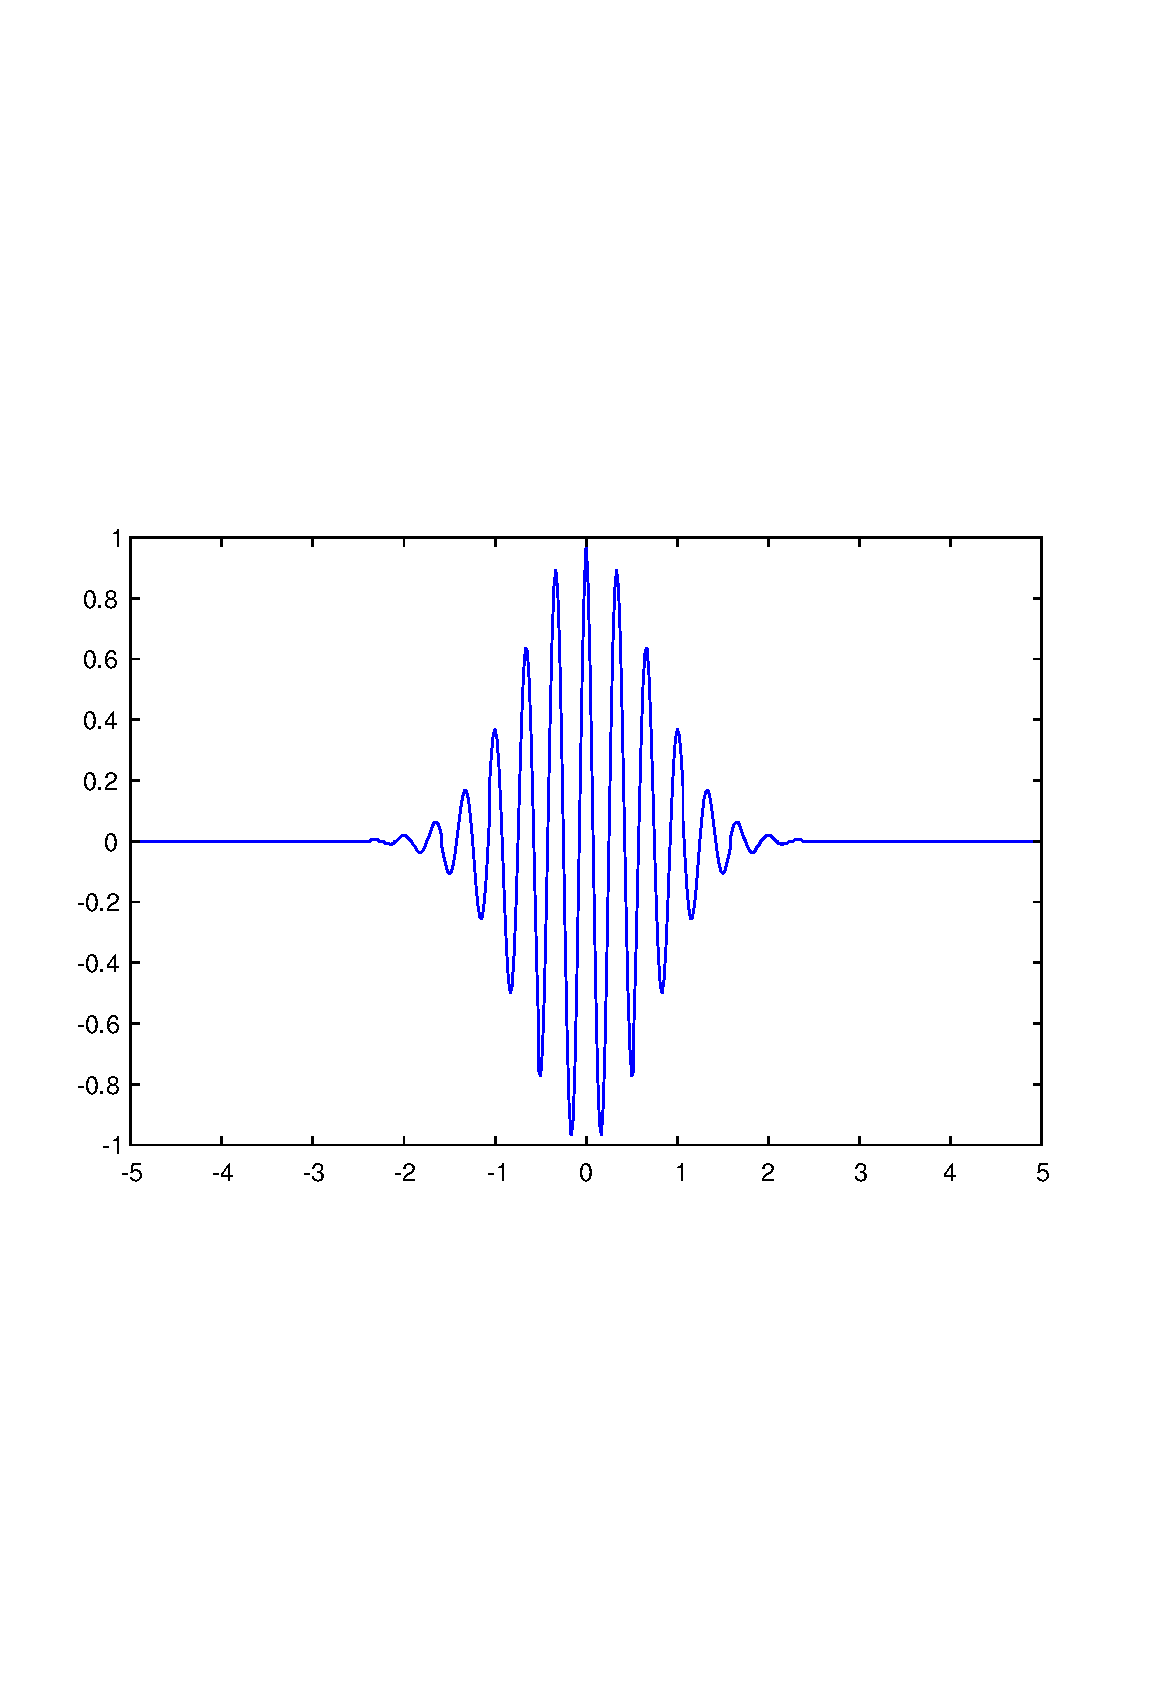
\includegraphics[width=12cm]{hold1}
\caption{hold1}
\end{DoxyImage}


We now turn the hold state to {\ttfamily 'on'}, and add another plot sequence, this time composed of the top and bottom envelopes of the modulated Gaussian. We add the two envelopes simultaneously using a single {\ttfamily plot} command. The fact that {\ttfamily hold} is {\ttfamily 'on'} means that these two envelopes are added to (instead of replace) the current contents of the plot.


\begin{DoxyVerbInclude}
--> plot(x,y);
--> hold on
--> plot(x,t,'g-',x,-t,'b-')
\end{DoxyVerbInclude}


 
\begin{DoxyImage}
\includegraphics[width=12cm]{hold2}
\caption{hold2}
\end{DoxyImage}
 \hypertarget{handle_hpatch}{}\section{H\-P\-A\-T\-C\-H Create a patch object}\label{handle_hpatch}
Section\-: \hyperlink{sec_handle}{Handle-\/\-Based Graphics} \hypertarget{vtkwidgets_vtkxyplotwidget_Usage}{}\subsection{Usage}\label{vtkwidgets_vtkxyplotwidget_Usage}
Creates a patch object and parents it to the current axis. The syntax for its use is \begin{DoxyVerb}  handle = hpatch(property,value,property,value,...)
\end{DoxyVerb}
 where {\ttfamily property} and {\ttfamily value} are set. The handle I\-D for the resulting object is returned. It is automatically added to the children of the current axis. \hypertarget{handle_hpoint}{}\section{H\-P\-O\-I\-N\-T Get Point From Window}\label{handle_hpoint}
Section\-: \hyperlink{sec_handle}{Handle-\/\-Based Graphics} \hypertarget{vtkwidgets_vtkxyplotwidget_Usage}{}\subsection{Usage}\label{vtkwidgets_vtkxyplotwidget_Usage}
This function waits for the user to click on the current figure window, and then returns the coordinates of that click. The generic syntax for its use is \begin{DoxyVerb}  [x,y] = hpoint
\end{DoxyVerb}
 \hypertarget{handle_hrawplot}{}\section{H\-R\-A\-W\-P\-L\-O\-T Generate a Raw Plot File}\label{handle_hrawplot}
Section\-: \hyperlink{sec_handle}{Handle-\/\-Based Graphics} \hypertarget{vtkwidgets_vtkxyplotwidget_Usage}{}\subsection{Usage}\label{vtkwidgets_vtkxyplotwidget_Usage}
This function takes a sequence of commands, and generates a raw plot (to a file) that renders the commands. It is a useful tool for creating high quality fully customized P\-D\-F plots from within Free\-Mat scripts that are portable. The syntax for its use \begin{DoxyVerb}  hrawplot(filename,commands)
\end{DoxyVerb}
 where {\ttfamily filename} is the name of the file to plot to, and {\ttfamily commands} is a cell array of strings. Each entry in the cell array contains a string with a command text. The commands describe a simple mini-\/language for describing plots. The complete dictionary of commands is given 
\begin{DoxyItemize}
\item {\ttfamily L\-I\-N\-E x1 y1 x2 y2} -- draw a line  
\item {\ttfamily F\-O\-N\-T name size} -- select a font of the given name and size  
\item {\ttfamily T\-E\-X\-T x1 y1 string} -- draw the given text string at the given location  
\item {\ttfamily S\-T\-Y\-L\-E style} -- select line style ('solid' or 'dotted')  
\item {\ttfamily P\-A\-G\-E} -- force a new page  
\item {\ttfamily S\-I\-Z\-E x1 y1} -- Set the page mapping  
\item {\ttfamily B\-O\-X x1 y1 x2 y2} -- draw a filled box covering the given coordinates  
\item {\ttfamily H\-T\-E\-X\-T\-B\-O\-X x1 y1 x2 y2 string} -- Draw a horizontal box with the given string centered in it  
\item {\ttfamily V\-T\-E\-X\-T\-B\-O\-X x1 y1 x2 y2 string} -- Draw a vertical box with the given string centered in it (rotated 90 degrees)  
\item {\ttfamily B\-R\-U\-S\-H string} -- Set the brush color ('red','blue', etc)  
\item {\ttfamily P\-E\-N string} -- Set the pen color  
\end{DoxyItemize}\hypertarget{handle_hsurface}{}\section{H\-S\-U\-R\-F\-A\-C\-E Create a surface object}\label{handle_hsurface}
Section\-: \hyperlink{sec_handle}{Handle-\/\-Based Graphics} \hypertarget{vtkwidgets_vtkxyplotwidget_Usage}{}\subsection{Usage}\label{vtkwidgets_vtkxyplotwidget_Usage}
Creates a surface object and parents it to the current axis. The syntax for its use is \begin{DoxyVerb}  handle = hsurface(property,value,property,value,...)
\end{DoxyVerb}
 where {\ttfamily property} and {\ttfamily value} are set. The handle I\-D for the resulting object is returned. It is automatically added to the children of the current axis. \hypertarget{handle_htext}{}\section{H\-T\-E\-X\-T Create a text object}\label{handle_htext}
Section\-: \hyperlink{sec_handle}{Handle-\/\-Based Graphics} \hypertarget{vtkwidgets_vtkxyplotwidget_Usage}{}\subsection{Usage}\label{vtkwidgets_vtkxyplotwidget_Usage}
Creates a text object and parents it to the current axis. The syntax for its use is \begin{DoxyVerb}  handle = htext(property,value,property,value,...)
\end{DoxyVerb}
 where {\ttfamily property} and {\ttfamily value} are set. The handle I\-D for the resulting object is returned. It is automatically added to the children of the current axis. \hypertarget{handle_htextbitmap}{}\section{H\-T\-E\-X\-T\-B\-I\-T\-M\-A\-P Get Text Rendered as a Bitmap}\label{handle_htextbitmap}
Section\-: \hyperlink{sec_handle}{Handle-\/\-Based Graphics} \hypertarget{vtkwidgets_vtkxyplotwidget_Usage}{}\subsection{Usage}\label{vtkwidgets_vtkxyplotwidget_Usage}
This function takes a fontname, a size, and a text string and returns a bitmap containing the text. The generic syntax for its use is \begin{DoxyVerb}  bitmap = htextbitmap(fontname,size,text)
\end{DoxyVerb}
 where the output bitmap contains the text rendered into a matrix. \hypertarget{handle_image}{}\section{I\-M\-A\-G\-E Image Display Function}\label{handle_image}
Section\-: \hyperlink{sec_handle}{Handle-\/\-Based Graphics} \hypertarget{vtkwidgets_vtkxyplotwidget_Usage}{}\subsection{Usage}\label{vtkwidgets_vtkxyplotwidget_Usage}
The {\ttfamily image} command has the following general syntax \begin{DoxyVerb}  handle = image(x,y,C,properties...)
\end{DoxyVerb}
 where {\ttfamily x} is a two vector containing the {\ttfamily x} coordinates of the first and last pixels along a column, and {\ttfamily y} is a two vector containing the {\ttfamily y} coordinates of the first and last pixels along a row. The matrix {\ttfamily C} constitutes the image data. It must either be a scalar matrix, in which case the image is colormapped using the {\ttfamily colormap} for the current figure. If the matrix is {\ttfamily M x N x 3}, then {\ttfamily C} is intepreted as R\-G\-B data, and the image is not colormapped. The {\ttfamily properties} argument is a set of {\ttfamily property/value} pairs that affect the final image. You can also omit the {\ttfamily x} and {\ttfamily y}, \begin{DoxyVerb}  handle = image(C, properties...)
\end{DoxyVerb}
 in which case they default to {\ttfamily x = \mbox{[}1,size(\-C,2)\mbox{]}} and {\ttfamily y = \mbox{[}1,size(\-C,1)\mbox{]}}. Finally, you can use the {\ttfamily image} function with only formal arguments \begin{DoxyVerb}  handle = image(properties...)
\end{DoxyVerb}


To support legacy Free\-Mat code, you can also use the following form of {\ttfamily image} \begin{DoxyVerb}  image(C, zoomfactor)
\end{DoxyVerb}
 which is equivalent to {\ttfamily image(\-C)} with the axes removed so that the image takes up the full figure window, and the size of the figure window adjusted to achieve the desired zoom factor using the {\ttfamily zoom} command. \hypertarget{variables_struct_Example}{}\subsection{Example}\label{variables_struct_Example}
In this example, we create an image that is {\ttfamily 512 x 512} pixels square, and set the background to a noise pattern. We set the central {\ttfamily 128 x 256} pixels to be white.


\begin{DoxyVerbInclude}
--> x = rand(512);
--> x((-64:63)+256,(-128:127)+256) = 1.0;
--> figure

ans = 
 1 

--> image(x)
--> colormap(gray)
\end{DoxyVerbInclude}


The resulting image looks like\-:  
\begin{DoxyImage}
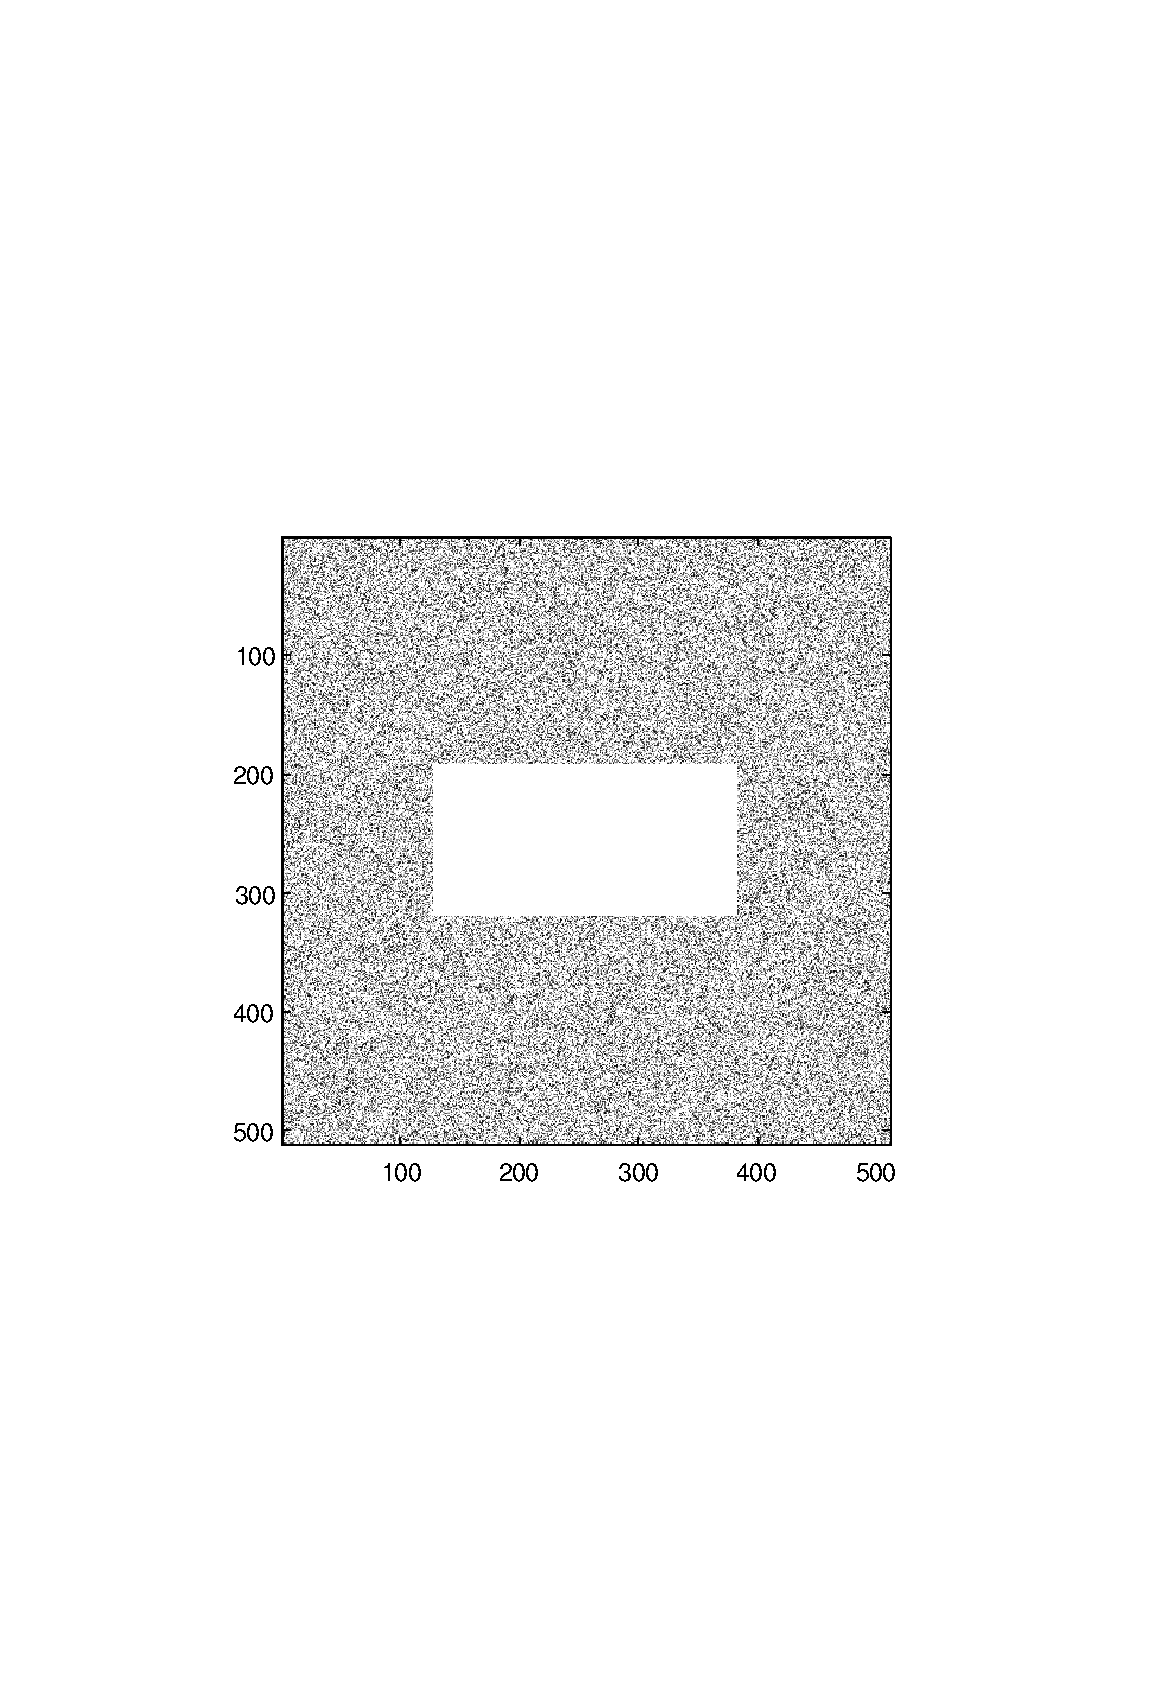
\includegraphics[width=12cm]{image1}
\caption{image1}
\end{DoxyImage}
 Here is an example of an R\-G\-B image


\begin{DoxyVerbInclude}
--> t = linspace(0,1);
--> red = t'*t;
--> green = t'*(t.^2);
--> blue = t'*(0*t+1);
--> A(:,:,1) = red; 
--> A(:,:,2) = green; 
--> A(:,:,3) = blue;
--> image(A);
\end{DoxyVerbInclude}


The resulting image looks like\-:  
\begin{DoxyImage}
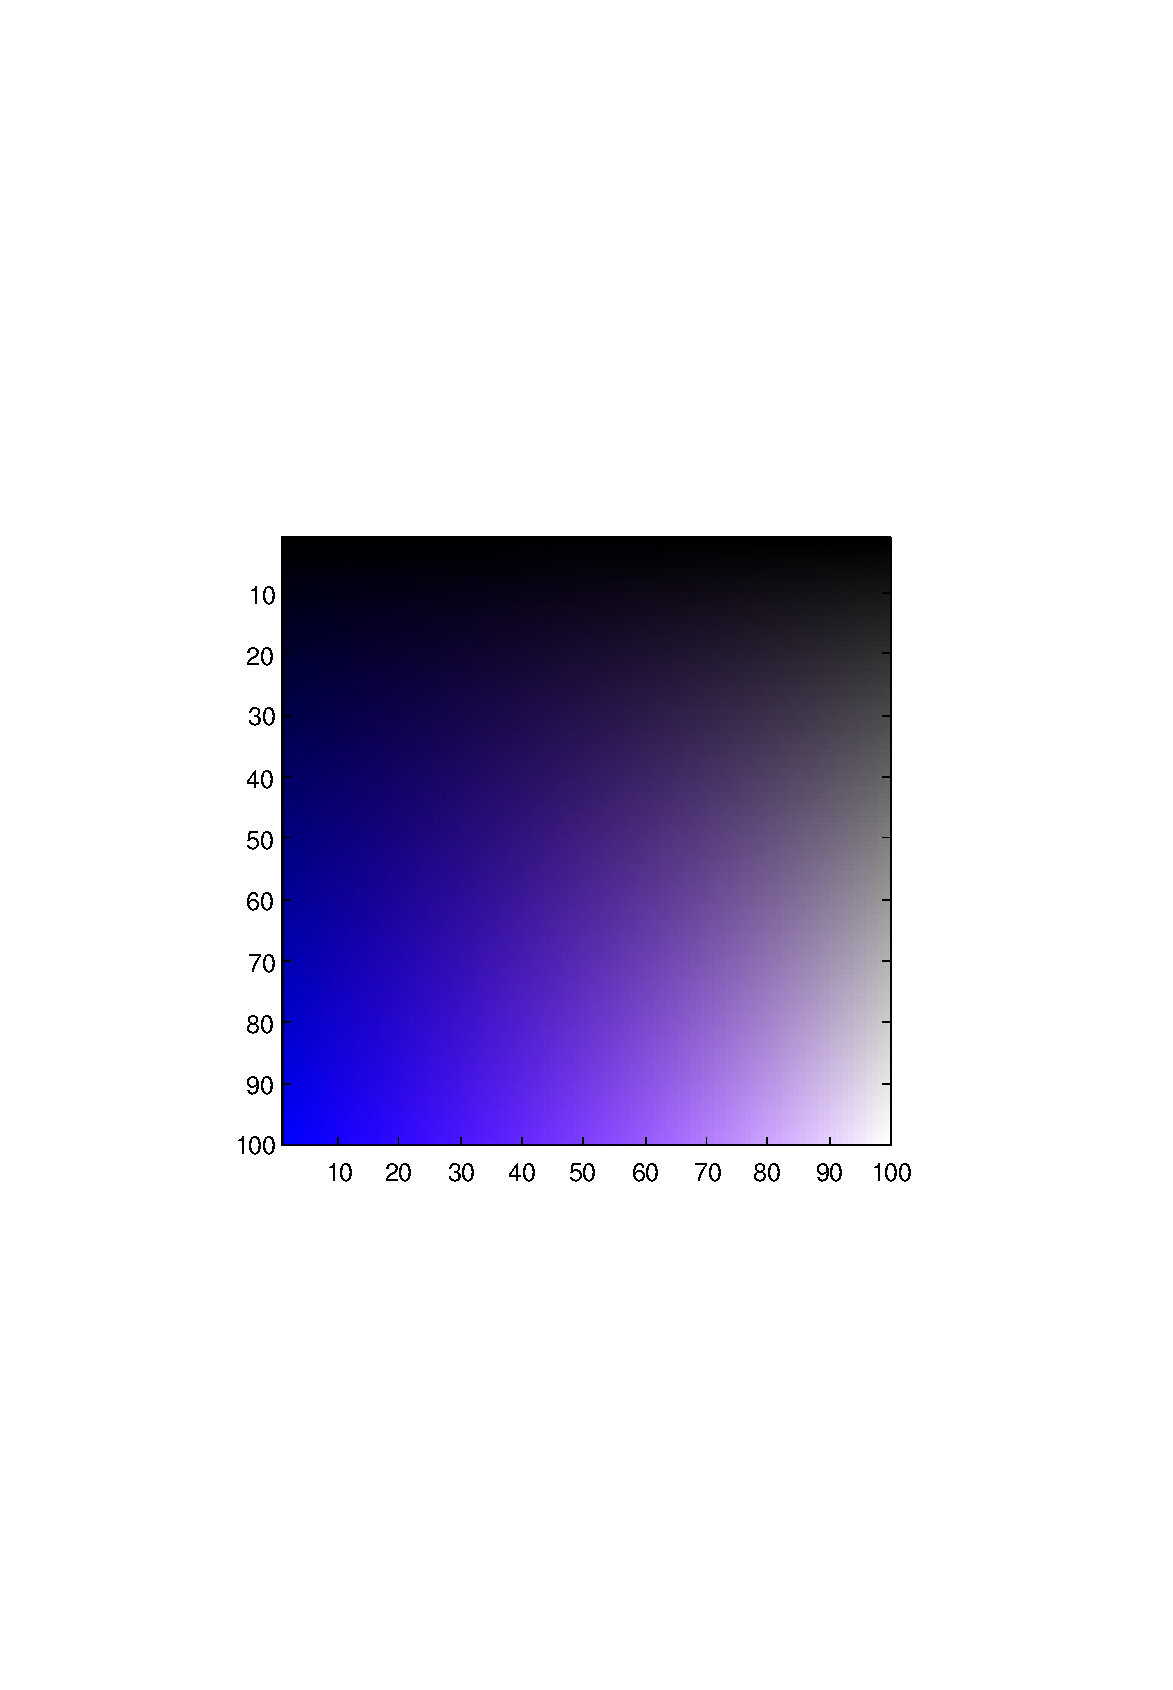
\includegraphics[width=12cm]{image2}
\caption{image2}
\end{DoxyImage}
 \hypertarget{handle_imageproperties}{}\section{I\-M\-A\-G\-E\-P\-R\-O\-P\-E\-R\-T\-I\-E\-S Image Object Properties}\label{handle_imageproperties}
Section\-: \hyperlink{sec_handle}{Handle-\/\-Based Graphics} \hypertarget{vtkwidgets_vtkxyplotwidget_Usage}{}\subsection{Usage}\label{vtkwidgets_vtkxyplotwidget_Usage}
Below is a summary of the properties for the axis. 
\begin{DoxyItemize}
\item {\ttfamily alphadata} -\/ {\ttfamily vector} -\/ This is a vector that should contain as many elements as the image data itself {\ttfamily cdata}, or a single scalar. For a single scalar, all values of the image take on the same transparency. Otherwise, the transparency of each pixel is determined by the corresponding value from the {\ttfamily alphadata} vector.  
\item {\ttfamily alphadatamapping} -\/ {\ttfamily \{'scaled','direct','none'\}} -\/ For {\ttfamily none} mode (the default), no transparency is applied to the data. For {\ttfamily direct} mode, the vector {\ttfamily alphadata} contains values between @\mbox{[}0,M-\/1\mbox{]}$|$ where {\ttfamily M} is the length of the alpha map stored in the figure. For {\ttfamily scaled} mode, the {\ttfamily alim} vector for the figure is used to linearly rescale the alpha data prior to lookup in the alpha map.  
\item {\ttfamily cdata} -\/ {\ttfamily array} -\/ This is either a {\ttfamily M x N} array or an {\ttfamily M x N x 3} array. If the data is {\ttfamily M x N} the image is a scalar image (indexed mode), where the color associated with each image pixel is computed using the colormap and the {\ttfamily cdatamapping} mode. If the data is {\ttfamily M x N x 3} the image is assumed to be in R\-G\-B mode, and the colorpanes are taken directly from {\ttfamily cdata} (the colormap is ignored). Note that in this case, the data values must be between @\mbox{[}0,1\mbox{]}$|$ for each color channel and each pixel.  
\item {\ttfamily cdatamapping} -\/ {\ttfamily \{'scaled','direct'\}} -\/ For {\ttfamily scaled} (the default), the pixel values are scaled using the {\ttfamily clim} vector for the figure prior to looking up in the colormap. For {\ttfamily direct} mode, the pixel values must be in the range {\ttfamily \mbox{[}0,N-\/1} where {\ttfamily N} is the number of colors in the colormap if the data is integer type. For floating point data types, values must be in the range {\ttfamily \mbox{[}1,N\mbox{]}}.  
\item {\ttfamily children} -\/ Not used.  
\item {\ttfamily parent} -\/ {\ttfamily handle} -\/ The axis containing the image.  
\item {\ttfamily tag} -\/ {\ttfamily string} -\/ You can set this to any string you want.  
\item {\ttfamily type} -\/ {\ttfamily string} -\/ Set to the string {\ttfamily 'image'}.  
\item {\ttfamily xdata} -\/ {\ttfamily two vector} -\/ contains the x coordinates of the first and last column (respectively). Defaults to {\ttfamily \mbox{[}1,C\mbox{]}} where {\ttfamily C} is the number of columns in the image.  
\item {\ttfamily ydata} -\/ {\ttfamily two vector} -\/ contains the y coordinates of the first and last row (respectively). Defaults to {\ttfamily \mbox{[}1,R\mbox{]}} where {\ttfamily R} is the number of rows in the image.  
\item {\ttfamily userdata} -\/ {\ttfamily array} -\/ Available to store any variable you want in the handle object.  
\item {\ttfamily visible} -\/ {\ttfamily \{'on','off'\}} -\/ Controls whether the image is visible or not.  
\end{DoxyItemize}\hypertarget{handle_imagesc}{}\section{I\-M\-A\-G\-E\-S\-C Image Display Function}\label{handle_imagesc}
Section\-: \hyperlink{sec_handle}{Handle-\/\-Based Graphics} \hypertarget{vtkwidgets_vtkxyplotwidget_Usage}{}\subsection{Usage}\label{vtkwidgets_vtkxyplotwidget_Usage}
The {\ttfamily imagesc} command has the following general syntax \begin{DoxyVerb}  handle = imagesc(x,y,C,clim)
\end{DoxyVerb}
 where {\ttfamily x} is a two vector containing the {\ttfamily x} coordinates of the first and last pixels along a column, and {\ttfamily y} is a two vector containing the {\ttfamily y} coordinates of the first and last pixels along a row. The matrix {\ttfamily C} constitutes the image data. It must either be a scalar matrix, in which case the image is colormapped using the {\ttfamily colormap} for the current figure. If the matrix is {\ttfamily M x N x 3}, then {\ttfamily C} is intepreted as R\-G\-B data, and the image is not colormapped. The {\ttfamily clim} argument is a pairs \mbox{[}low high\mbox{]} that specifies scaling. You can also omit the {\ttfamily x} and {\ttfamily y}, \begin{DoxyVerb}  handle = imagesc(C, clim)
\end{DoxyVerb}
 in which case they default to {\ttfamily x = \mbox{[}1,size(\-C,2)\mbox{]}} and {\ttfamily y = \mbox{[}1,size(\-C,1)\mbox{]}}. Finally, you can use the {\ttfamily image} function with only formal arguments \begin{DoxyVerb}  handle = imagesc(properties...)
\end{DoxyVerb}
\hypertarget{variables_struct_Example}{}\subsection{Example}\label{variables_struct_Example}
In this example, we create an image that is {\ttfamily 512 x 512} pixels square, and set the background to a noise pattern. We set the central {\ttfamily 128 x 256} pixels to be white.


\begin{DoxyVerbInclude}
--> x = rand(512);
--> x((-64:63)+256,(-128:127)+256) = 1.0;
--> figure

ans = 
 1 

--> imagesc(x,[0 .5])
--> colormap(gray)
\end{DoxyVerbInclude}
 \hypertarget{handle_is2dview}{}\section{I\-S2\-D\-V\-I\-E\-W Test Axes For 2\-D View}\label{handle_is2dview}
Section\-: \hyperlink{sec_handle}{Handle-\/\-Based Graphics} \hypertarget{vtkwidgets_vtkxyplotwidget_Usage}{}\subsection{Usage}\label{vtkwidgets_vtkxyplotwidget_Usage}
This function returns {\ttfamily true} if the current axes are in a 2-\/\-D view, and false otherwise. The generic syntax for its use is \begin{DoxyVerb}  y = is2dview(x)
\end{DoxyVerb}
 where {\ttfamily x} is the handle of an axes object. \hypertarget{handle_ishold}{}\section{I\-S\-H\-O\-L\-D Test Hold Status}\label{handle_ishold}
Section\-: \hyperlink{sec_handle}{Handle-\/\-Based Graphics} \hypertarget{vtkwidgets_vtkxyplotwidget_Usage}{}\subsection{Usage}\label{vtkwidgets_vtkxyplotwidget_Usage}
Returns the state of the {\ttfamily hold} flag on the currently active plot. The general syntax for its use is \begin{DoxyVerb}   ishold
\end{DoxyVerb}
 and it returns a logical 1 if {\ttfamily hold} is {\ttfamily on}, and a logical 0 otherwise. \hypertarget{handle_legend}{}\section{L\-E\-G\-E\-N\-D Add Legent to Plot}\label{handle_legend}
Section\-: \hyperlink{sec_handle}{Handle-\/\-Based Graphics} \hypertarget{vtkwidgets_vtkxyplotwidget_Usage}{}\subsection{Usage}\label{vtkwidgets_vtkxyplotwidget_Usage}
This command adds a legend to the current plot. Currently, the following forms of the {\ttfamily legend} command are supported. The first form creates a legend with the given labels for the data series\-: \begin{DoxyVerb}  legend('label1','label2',...)
\end{DoxyVerb}
 where {\ttfamily 'label1'} is the text label associated with data plot 1 and so on. You can also use the {\ttfamily legend} command to control the appearance of the legend in the current plot. To remove the legend from the current plot, use \begin{DoxyVerb}  legend('off')
\end{DoxyVerb}
 To hide the legend for the current plot (but do not remove it) \begin{DoxyVerb}  legend('hide')
\end{DoxyVerb}
 And to show the legend that has been hidden, use \begin{DoxyVerb}  legend('show')
\end{DoxyVerb}
 You can also toggle the display of the box surrounding the legend. Use \begin{DoxyVerb}  legend('boxoff')
\end{DoxyVerb}
 or \begin{DoxyVerb}  legend('boxon')
\end{DoxyVerb}
 to turn the legend box off or on, respectively. To toggle the visible state of the current legend, use \begin{DoxyVerb}  legend('toggle')
\end{DoxyVerb}
 Specifying no arguments at all (apart from an optional location argument as specified below) results in the legend being rebuilt. This form is useful for picking up font changes or relocating the legend. \begin{DoxyVerb}  legend
\end{DoxyVerb}
 By default, the {\ttfamily legend} command places the new legend in the upper right corner of the current plot. To change this behavior, use the {\ttfamily 'location'} specifier (must be the last two options to the command) \begin{DoxyVerb}  legend(...,'location',option)
\end{DoxyVerb}
 where {\ttfamily option} takes on the following possible values 
\begin{DoxyItemize}
\item {\ttfamily north},{\ttfamily N} -\/ top center of plot  
\item {\ttfamily south},{\ttfamily S} -\/ bottom center of plot  
\item {\ttfamily east},{\ttfamily E} -\/ middle right of plot  
\item {\ttfamily west},{\ttfamily W} -\/ middle left of plot  
\item {\ttfamily northeast},{\ttfamily N\-E} -\/ top right of plot (default behavior)  
\item {\ttfamily northwest},{\ttfamily N\-W} -\/ top left of plot  
\item {\ttfamily southeast},{\ttfamily S\-E} -\/ bottom right of plot  
\item {\ttfamily southwest},{\ttfamily S\-W} -\/ bottom left of plot  
\end{DoxyItemize}This implementation of {\ttfamily legend} is incomplete relative to the M\-A\-T\-L\-A\-B A\-P\-I. The functionality will be improved in future versions of Free\-Mat. \hypertarget{handle_line}{}\section{L\-I\-N\-E Line Display Function}\label{handle_line}
Section\-: \hyperlink{sec_handle}{Handle-\/\-Based Graphics} \hypertarget{vtkwidgets_vtkxyplotwidget_Usage}{}\subsection{Usage}\label{vtkwidgets_vtkxyplotwidget_Usage}
The {\ttfamily line} command has the following general syntax \begin{DoxyVerb}   handle = line(x,y,z,properties...)
\end{DoxyVerb}
 where... \hypertarget{handle_lineproperties}{}\section{L\-I\-N\-E\-P\-R\-O\-P\-E\-R\-T\-I\-E\-S Line Series Object Properties}\label{handle_lineproperties}
Section\-: \hyperlink{sec_handle}{Handle-\/\-Based Graphics} \hypertarget{vtkwidgets_vtkxyplotwidget_Usage}{}\subsection{Usage}\label{vtkwidgets_vtkxyplotwidget_Usage}
Below is a summary of the properties for a line series. 
\begin{DoxyItemize}
\item {\ttfamily color} -\/ {\ttfamily colorspec} -\/ The color that is used to draw the line.  
\item {\ttfamily children} -\/ Not used.  
\item {\ttfamily displayname} -\/ The name of this line series as it appears in a legend.  
\item {\ttfamily linestyle} -\/ {\ttfamily \{'-\/','--','\-:','-\/.','none'\}} -\/ The style of the line.  
\item {\ttfamily linewidth} -\/ {\ttfamily scalar} -\/ The width of the line.  
\item {\ttfamily marker} -\/ {\ttfamily \{'+','o','$\ast$','.','x','square','s','diamond','d','$^\wedge$','v','$>$','$<$'\}} -\/ The marker for data points on the line. Some of these are redundant, as {\ttfamily 'square'} {\ttfamily 's'} are synonyms, and {\ttfamily 'diamond'} and {\ttfamily 'd'} are also synonyms.  
\item {\ttfamily markeredgecolor} -\/ {\ttfamily colorspec} -\/ The color used to draw the marker. For some of the markers (circle, square, etc.) there are two colors used to draw the marker. This property controls the edge color (which for unfilled markers) is the primary color of the marker.  
\item {\ttfamily markerfacecolor} -\/ {\ttfamily colorspec} -\/ The color used to fill the marker. For some of the markers (circle, square, etc.) there are two colors used to fill the marker.  
\item {\ttfamily markersize} -\/ {\ttfamily scalar} -\/ Control the size of the marker. Defaults to 6, which is effectively the radius (in pixels) of the markers.  
\item {\ttfamily parent} -\/ {\ttfamily handle} -\/ The axis that contains this object.  
\item {\ttfamily tag} -\/ {\ttfamily string} -\/ A string that can be used to tag the object.  
\item {\ttfamily type} -\/ {\ttfamily string} -\/ Returns the string {\ttfamily 'line'}.  
\item {\ttfamily visible} -\/ {\ttfamily \{'on','off'\}} -\/ Controls visibility of the the line.  
\item {\ttfamily xdata} -\/ {\ttfamily vector} -\/ Vector of x coordinates of points on the line. Must be the same size as the {\ttfamily ydata} and {\ttfamily zdata} vectors.  
\item {\ttfamily ydata} -\/ {\ttfamily vector} -\/ Vector of y coordinates of points on the line. Must be the same size as the {\ttfamily xdata} and {\ttfamily zdata} vectors.  
\item {\ttfamily zdata} -\/ {\ttfamily vector} -\/ Vector of z coordinates of points on the line. Must be the same size as the {\ttfamily xdata} and {\ttfamily ydata} vectors.  
\item {\ttfamily xdatamode} -\/ {\ttfamily \{'auto','manual'\}} -\/ When set to {\ttfamily 'auto'} Free\-Mat will autogenerate the x coordinates for the points on the line. These values will be {\ttfamily 1,..,N} where {\ttfamily N} is the number of points in the line.  
\item {\ttfamily userdata} -\/ {\ttfamily array} -\/ Available to store any variable you want in the handle object.  
\end{DoxyItemize}\hypertarget{handle_loglog}{}\section{L\-O\-G\-L\-O\-G Log-\/\-Log Plot Function}\label{handle_loglog}
Section\-: \hyperlink{sec_handle}{Handle-\/\-Based Graphics} \hypertarget{vtkwidgets_vtkxyplotwidget_Usage}{}\subsection{Usage}\label{vtkwidgets_vtkxyplotwidget_Usage}
This command has the exact same syntax as the {\ttfamily plot} command\-: \begin{DoxyVerb}  loglog(<data 1>,{linespec 1},<data 2>,{linespec 2}...,properties...)
\end{DoxyVerb}
 in fact, it is a simple wrapper around {\ttfamily plot} that sets the x and y axis to have a logarithmic scale. \hypertarget{variables_struct_Example}{}\subsection{Example}\label{variables_struct_Example}
Here is an example of a doubly exponential signal plotted first on a linear plot\-:


\begin{DoxyVerbInclude}
--> x = linspace(1,100);
--> y = x;
--> plot(x,y,'r-');
\end{DoxyVerbInclude}


 
\begin{DoxyImage}
\includegraphics[width=12cm]{loglog1}
\caption{loglog1}
\end{DoxyImage}
 and now on a log-\/log plot


\begin{DoxyVerbInclude}
--> loglog(x,y,'r-');
\end{DoxyVerbInclude}


 
\begin{DoxyImage}
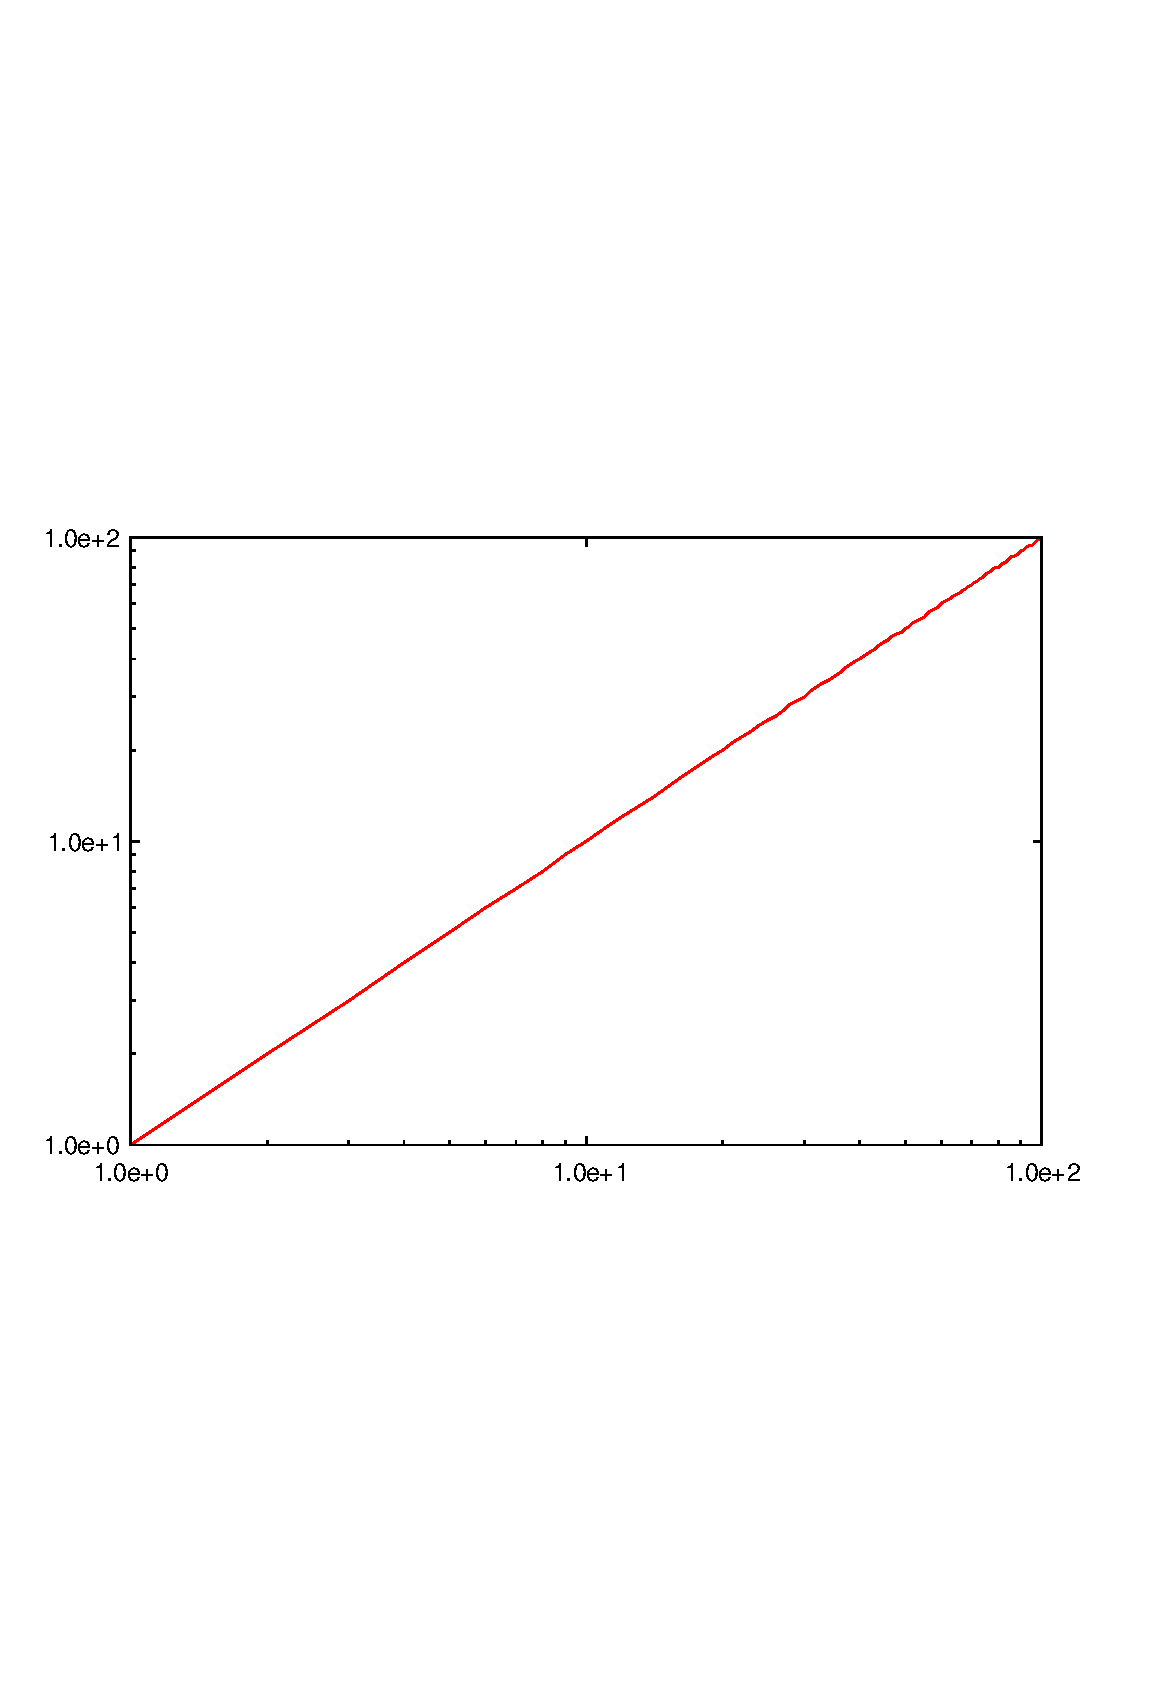
\includegraphics[width=12cm]{loglog2}
\caption{loglog2}
\end{DoxyImage}
 \hypertarget{handle_newplot}{}\section{N\-E\-W\-P\-L\-O\-T Get Handle For Next Plot}\label{handle_newplot}
Section\-: \hyperlink{sec_handle}{Handle-\/\-Based Graphics} \hypertarget{vtkwidgets_vtkxyplotwidget_Usage}{}\subsection{Usage}\label{vtkwidgets_vtkxyplotwidget_Usage}
Returns the handle for the next plot operation. The general syntax for its use is \begin{DoxyVerb}  h = newplot
\end{DoxyVerb}
 This routine checks the {\ttfamily nextplot} properties of the current figure and axes to see if they are set to {\ttfamily replace} or not. If the figures {\ttfamily nextplot} property is set to replace, the current figure is cleared. If the axes {\ttfamily nextplot} property is set to {\ttfamily replace} then the axes are cleared for the next operation. \hypertarget{handle_patch}{}\section{P\-A\-T\-C\-H Patch Graphics Function}\label{handle_patch}
Section\-: \hyperlink{sec_handle}{Handle-\/\-Based Graphics} \hypertarget{vtkwidgets_vtkxyplotwidget_Usage}{}\subsection{Usage}\label{vtkwidgets_vtkxyplotwidget_Usage}
This routine is used to create a patch object that can be plotting 2\-D and 3\-D surfaces. A patch is a polygon defined by the xyz coordinates of its vertices and optionally by the color at the vertices. There are several forms for the {\ttfamily patch} function\-: \begin{DoxyVerb}  h = patch(X,Y,C,properties...)
  h = patch(X,Y,Z,C,properties...)
  h = patch(properties...)
  h = patch(V)
\end{DoxyVerb}
 Where {\ttfamily X}, {\ttfamily Y} and {\ttfamily Z} are matrices or vectors of {\ttfamily x}, {\ttfamily y} or {\ttfamily z} coordinates and {\ttfamily C} is a matrix or vector of color values (the colormap for the current fig is applied). \hypertarget{variables_struct_Example}{}\subsection{Example}\label{variables_struct_Example}
Here we generate a surface specifying all four components.


\begin{DoxyVerbInclude}
--> x = [ 0 1 0 1]';
--> y = [ 0 0 1 1]';
--> c = [ 1 1 1 ];
--> patch(x,y,c)
--> axis equal
--> view(3)
\end{DoxyVerbInclude}


 
\begin{DoxyImage}
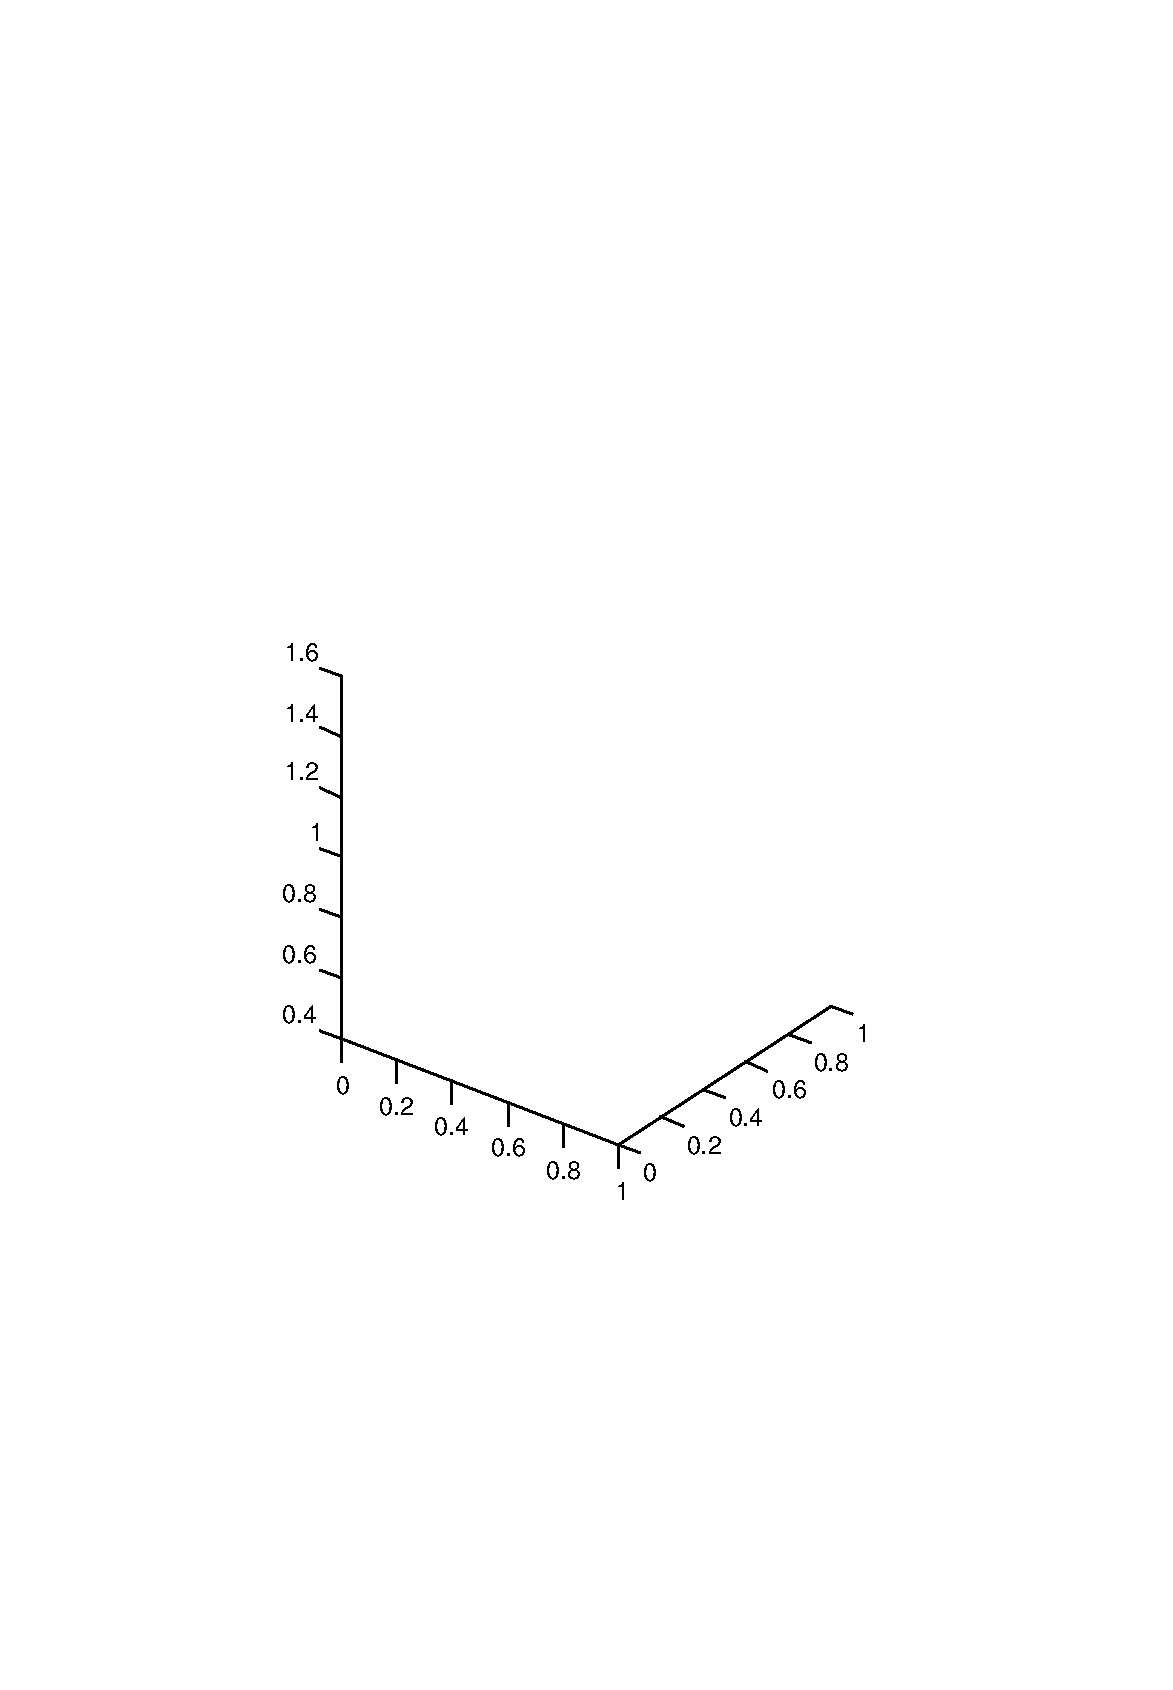
\includegraphics[width=12cm]{patch1}
\caption{patch1}
\end{DoxyImage}
 \hypertarget{handle_pcolor}{}\section{P\-C\-O\-L\-O\-R Pseudocolor Plot}\label{handle_pcolor}
Section\-: \hyperlink{sec_handle}{Handle-\/\-Based Graphics} \hypertarget{vtkwidgets_vtkxyplotwidget_Usage}{}\subsection{Usage}\label{vtkwidgets_vtkxyplotwidget_Usage}
This routine is used to create a pseudocolor plot of the data. A pseudocolor plot is a essentially a surface plot seen from above. There are two forms for the {\ttfamily pcolor} command\-: \begin{DoxyVerb}   pcolor(C)
\end{DoxyVerb}
 which uses a rectangular grid. Alternately, you can specify {\ttfamily X,Y} matrices or vectors. \begin{DoxyVerb}   pcolor(X,Y,C)
\end{DoxyVerb}
 \hypertarget{handle_plot}{}\section{P\-L\-O\-T Plot Function}\label{handle_plot}
Section\-: \hyperlink{sec_handle}{Handle-\/\-Based Graphics} \hypertarget{vtkwidgets_vtkxyplotwidget_Usage}{}\subsection{Usage}\label{vtkwidgets_vtkxyplotwidget_Usage}
This is the basic plot command for Free\-Mat. The general syntax for its use is \begin{DoxyVerb}  plot(\<data 1\>,{linespec 1},\<data 2\>,{linespec 2}...,properties...)
\end{DoxyVerb}
 where the {\ttfamily $<$data$>$} arguments can have various forms, and the {\ttfamily linespec} arguments are optional. We start with the {\ttfamily $<$data$>$} term, which can take on one of multiple forms\-: 
\begin{DoxyItemize}
\item Vector Matrix Case -- In this case the argument data is a pair of variables. A set of {\ttfamily x} coordinates in a numeric vector, and a set of {\ttfamily y} coordinates in the columns of the second, numeric matrix. {\ttfamily x} must have as many elements as {\ttfamily y} has columns (unless {\ttfamily y} is a vector, in which case only the number of elements must match). Each column of {\ttfamily y} is plotted sequentially against the common vector {\ttfamily x}.  
\item Unpaired Matrix Case -- In this case the argument data is a single numeric matrix {\ttfamily y} that constitutes the {\ttfamily y}-\/values of the plot. An {\ttfamily x} vector is synthesized as {\ttfamily x = 1\-:length(y)}, and each column of {\ttfamily y} is plotted sequentially against this common {\ttfamily x} axis.  
\item Complex Matrix Case -- Here the argument data is a complex matrix, in which case, the real part of each column is plotted against the imaginary part of each column. All columns receive the same line styles.  
\end{DoxyItemize}Multiple data arguments in a single plot command are treated as a {\bfseries sequence}, meaning that all of the plots are overlapped on the same set of axes. The {\ttfamily linespec} is a string used to change the characteristics of the line. In general, the {\ttfamily linespec} is composed of three optional parts, the {\ttfamily colorspec}, the {\ttfamily symbolspec} and the {\ttfamily linestylespec} in any order. Each of these specifications is a single character that determines the corresponding characteristic. First, the {\ttfamily colorspec}\-: 
\begin{DoxyItemize}
\item {\ttfamily 'b'} -\/ Color Blue  
\item {\ttfamily 'g'} -\/ Color Green  
\item {\ttfamily 'r'} -\/ Color Red  
\item {\ttfamily 'c'} -\/ Color Cyan  
\item {\ttfamily 'm'} -\/ Color Magenta  
\item {\ttfamily 'y'} -\/ Color Yellow  
\item {\ttfamily 'k'} -\/ Color Black  
\end{DoxyItemize}The {\ttfamily symbolspec} specifies the (optional) symbol to be drawn at each data point\-: 
\begin{DoxyItemize}
\item {\ttfamily '.'} -\/ Dot symbol  
\item {\ttfamily 'o'} -\/ Circle symbol  
\item {\ttfamily 'x'} -\/ Times symbol  
\item {\ttfamily '+'} -\/ Plus symbol  
\item {\ttfamily '$\ast$'} -\/ Asterisk symbol  
\item {\ttfamily 's'} -\/ Square symbol  
\item {\ttfamily 'd'} -\/ Diamond symbol  
\item {\ttfamily 'v'} -\/ Downward-\/pointing triangle symbol  
\item {\ttfamily '$^\wedge$'} -\/ Upward-\/pointing triangle symbol  
\item {\ttfamily '$<$'} -\/ Left-\/pointing triangle symbol  
\item {\ttfamily '$>$'} -\/ Right-\/pointing triangle symbol  
\end{DoxyItemize}The {\ttfamily linestylespec} specifies the (optional) line style to use for each data series\-: 
\begin{DoxyItemize}
\item {\ttfamily '-\/'} -\/ Solid line style  
\item {\ttfamily '\-:'} -\/ Dotted line style  
\item {\ttfamily '-\/.'} -\/ Dot-\/\-Dash-\/\-Dot-\/\-Dash line style  
\item {\ttfamily '--'} -\/ Dashed line style  
\end{DoxyItemize}For sequences of plots, the {\ttfamily linespec} is recycled with color order determined by the properties of the current axes. You can also use the {\ttfamily properties} argument to specify handle properties that will be inherited by all of the plots generated during this event. Finally, you can also specify the handle for the axes that are the target of the {\ttfamily plot} operation. \begin{DoxyVerb}  handle = plot(handle,...)
\end{DoxyVerb}
 \hypertarget{variables_struct_Example}{}\subsection{Example}\label{variables_struct_Example}
The most common use of the {\ttfamily plot} command probably involves the vector-\/matrix paired case. Here, we generate a simple cosine, and plot it using a red line, with no symbols (i.\-e., a {\ttfamily linespec} of {\ttfamily 'r-\/'}).


\begin{DoxyVerbInclude}
--> x = linspace(-pi,pi);
--> y = cos(x);
--> plot(x,y,'r-');
\end{DoxyVerbInclude}


which results in the following plot.  
\begin{DoxyImage}
\includegraphics[width=12cm]{plot1}
\caption{plot1}
\end{DoxyImage}


Next, we plot multiple sinusoids (at different frequencies). First, we construct a matrix, in which each column corresponds to a different sinusoid, and then plot them all at once.


\begin{DoxyVerbInclude}
--> x = linspace(-pi,pi);
--> y = [cos(x(:)),cos(3*x(:)),cos(5*x(:))];
--> plot(x,y);
\end{DoxyVerbInclude}


In this case, we do not specify a {\ttfamily linespec}, so that we cycle through the colors automatically (in the order listed in the previous section).  
\begin{DoxyImage}
\includegraphics[width=12cm]{plot2}
\caption{plot2}
\end{DoxyImage}


This time, we produce the same plot, but as we want to assign individual {\ttfamily linespec}s to each line, we use a sequence of arguments in a single plot command, which has the effect of plotting all of the data sets on a common axis, but which allows us to control the {\ttfamily linespec} of each plot. In the following example, the first line (harmonic) has red, solid lines with times symbols marking the data points, the second line (third harmonic) has blue, solid lines with right-\/pointing triangle symbols, and the third line (fifth harmonic) has green, dotted lines with asterisk symbols.


\begin{DoxyVerbInclude}
--> plot(x,y(:,1),'rx-',x,y(:,2),'b>-',x,y(:,3),'g*:');
\end{DoxyVerbInclude}


 
\begin{DoxyImage}
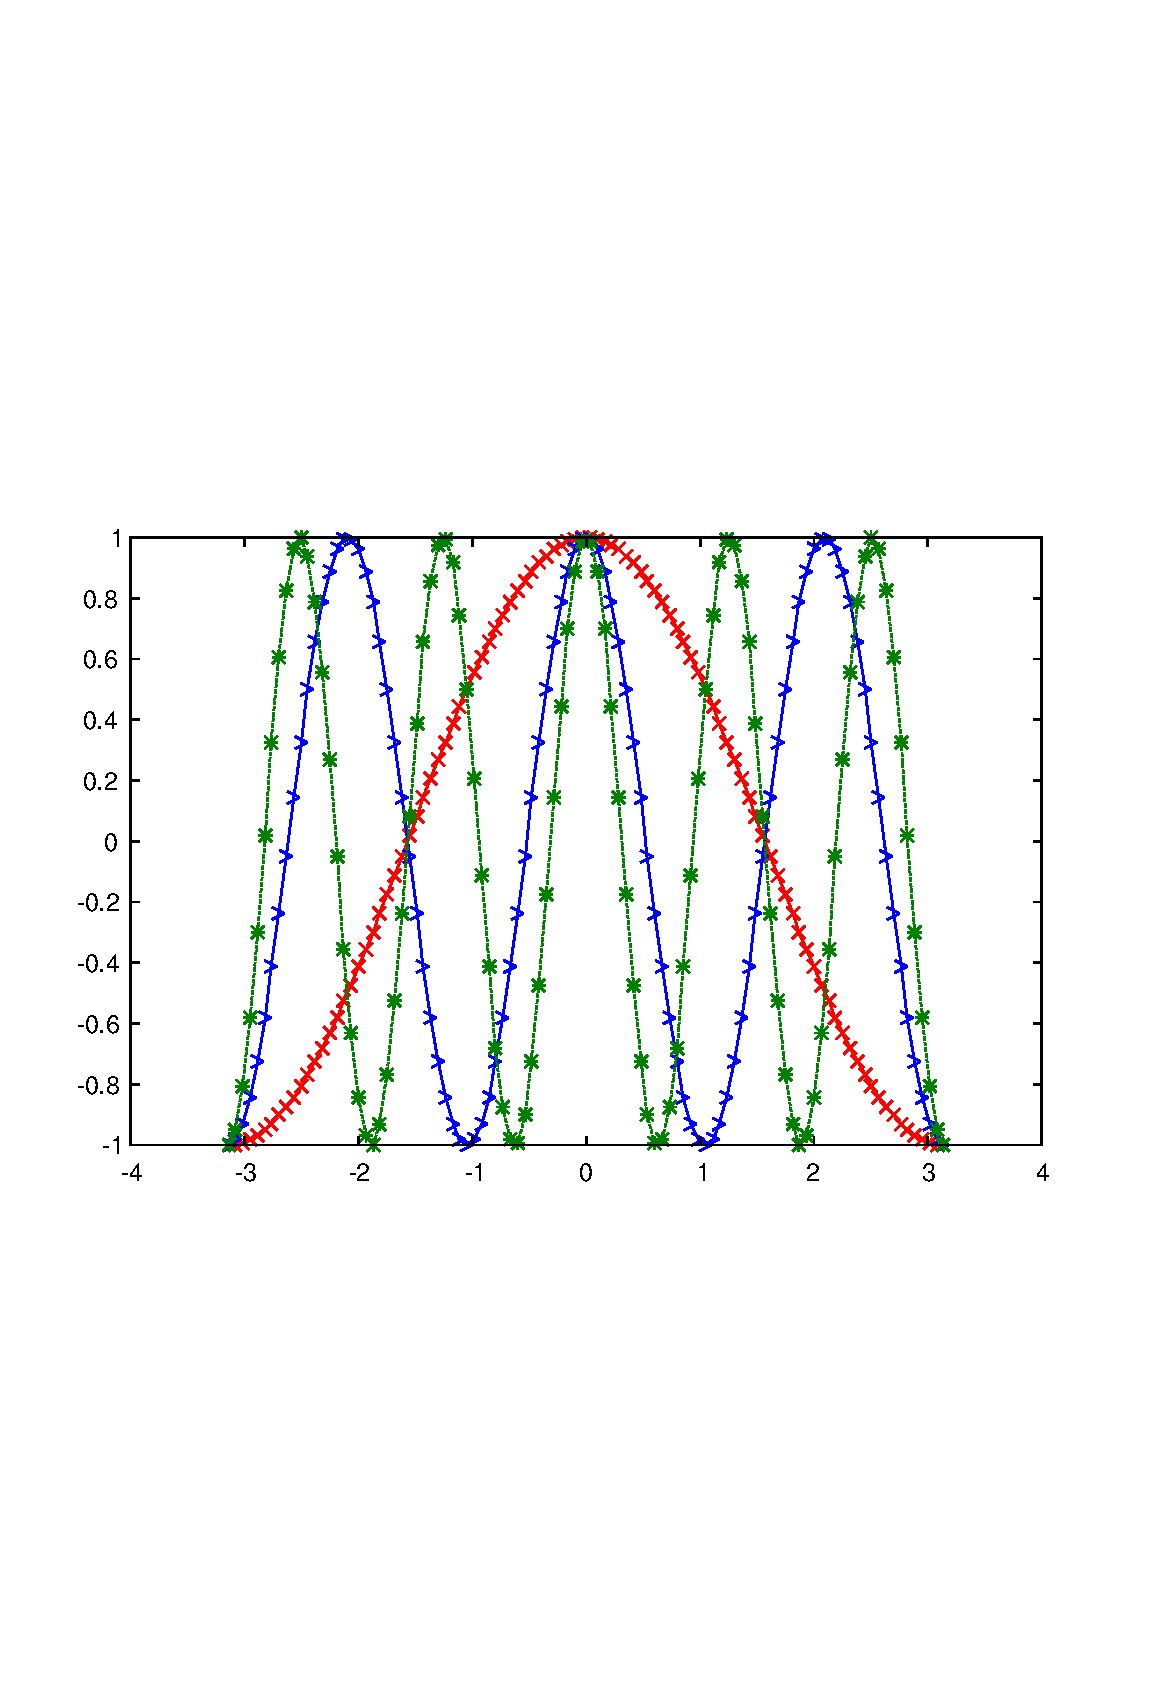
\includegraphics[width=12cm]{plot3}
\caption{plot3}
\end{DoxyImage}


The second most frequently used case is the unpaired matrix case. Here, we need to provide only one data component, which will be automatically plotted against a vector of natural number of the appropriate length. Here, we use a plot sequence to change the style of each line to be dotted, dot-\/dashed, and dashed.


\begin{DoxyVerbInclude}
--> plot(y(:,1),'r:',y(:,2),'b;',y(:,3),'g|');
\end{DoxyVerbInclude}


Note in the resulting plot that the {\ttfamily x}-\/axis no longer runs from {\ttfamily \mbox{[}-\/pi,pi\mbox{]}}, but instead runs from {\ttfamily \mbox{[}1,100\mbox{]}}.  
\begin{DoxyImage}
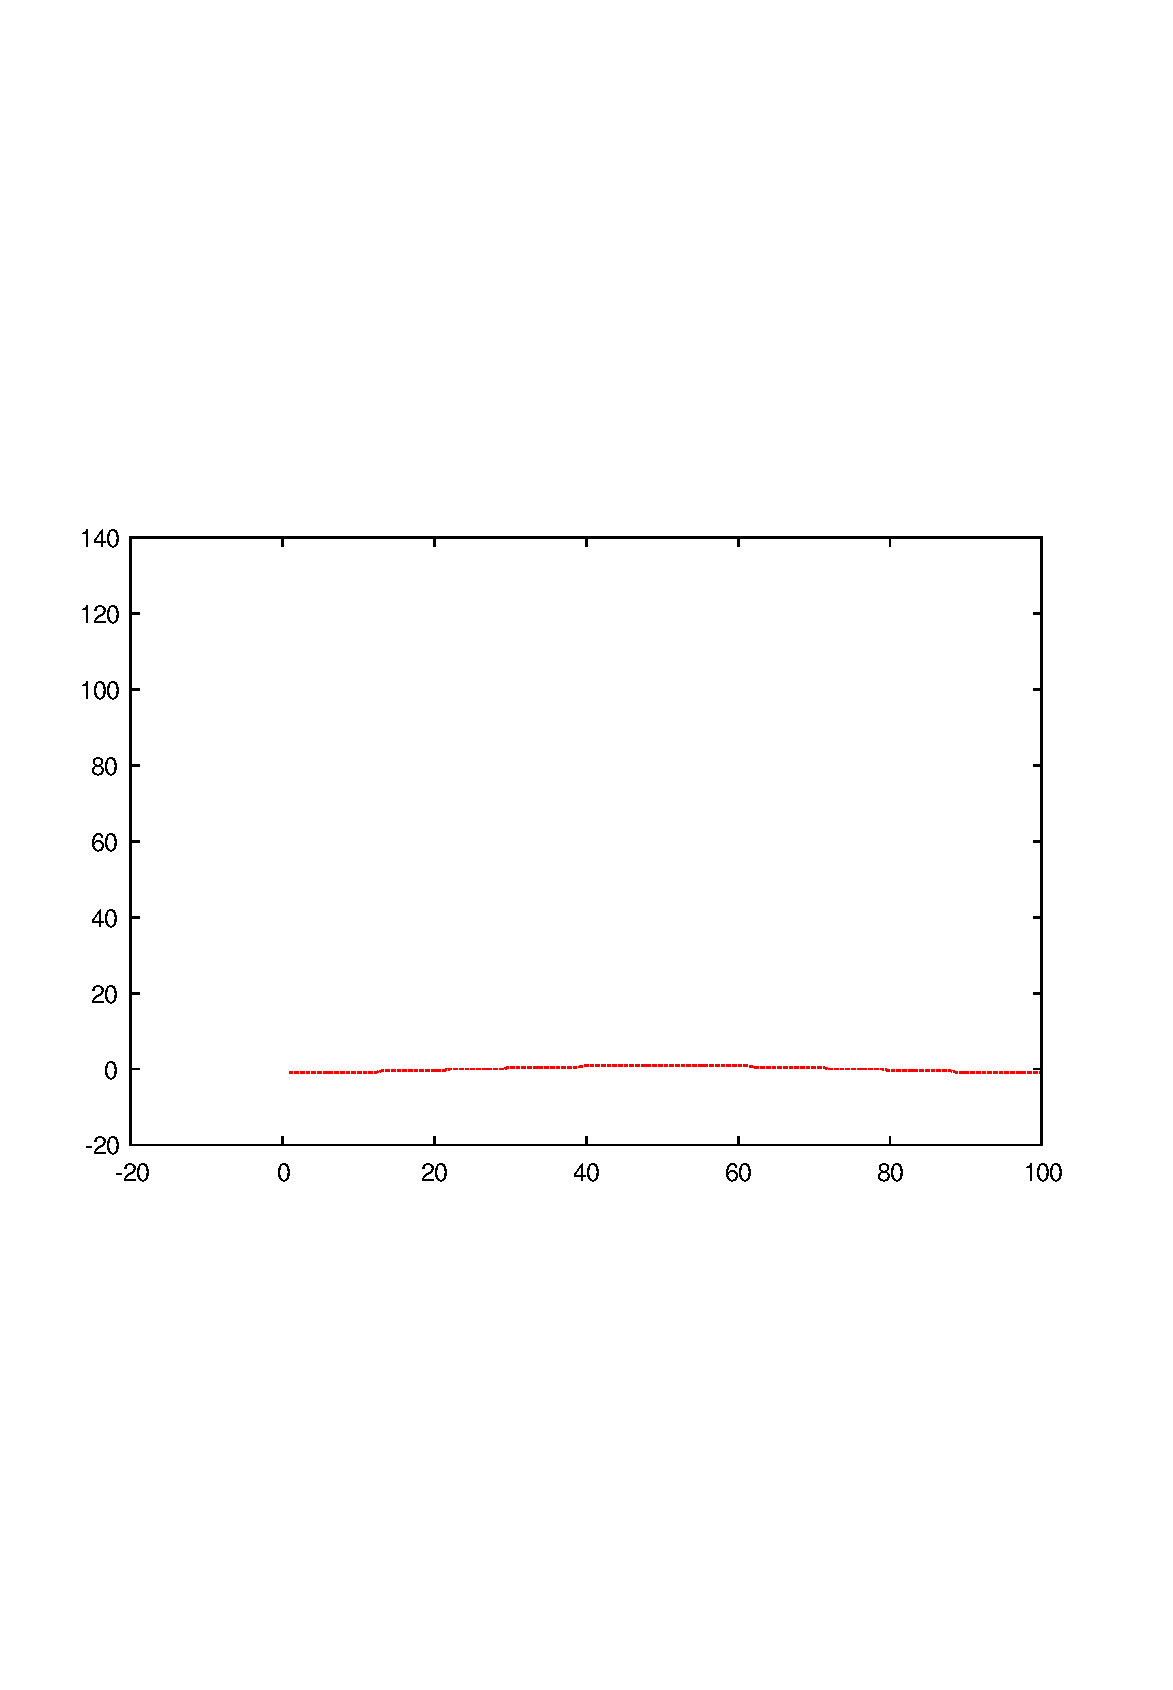
\includegraphics[width=12cm]{plot4}
\caption{plot4}
\end{DoxyImage}


The final case is for complex matrices. For complex arguments, the real part is plotted against the imaginary part. Hence, we can generate a 2-\/dimensional plot from a vector as follows.


\begin{DoxyVerbInclude}
--> y = cos(2*x) + i * cos(3*x);
--> plot(y);
\end{DoxyVerbInclude}


 
\begin{DoxyImage}
\includegraphics[width=12cm]{plot5}
\caption{plot5}
\end{DoxyImage}


Here is an example of using the handle properties to influence the behavior of the generated lines.


\begin{DoxyVerbInclude}
--> t = linspace(-3,3);
--> plot(cos(5*t).*exp(-t),'r-','linewidth',3);
\end{DoxyVerbInclude}


 
\begin{DoxyImage}
\includegraphics[width=12cm]{plot6}
\caption{plot6}
\end{DoxyImage}
 \hypertarget{handle_plot3}{}\section{P\-L\-O\-T3 Plot 3\-D Function}\label{handle_plot3}
Section\-: \hyperlink{sec_handle}{Handle-\/\-Based Graphics} \hypertarget{vtkwidgets_vtkxyplotwidget_Usage}{}\subsection{Usage}\label{vtkwidgets_vtkxyplotwidget_Usage}
This is the 3\-D plot command. The general syntax for its use is \begin{DoxyVerb}  plot3(X,Y,Z,{linespec 1},X,Y,Z,{linespec 2},...,properties...)
\end{DoxyVerb}
 where {\ttfamily X} {\ttfamily Y} and {\ttfamily Z} are the coordinates of the points on the 3\-D line. Note that in general, all three should be vectors. If some or all of the quantities are matrices, then Free\-Mat will attempt to expand the vector arguments to the same size, and then generate multiple plots, one for each column of the matrices. The linespec is optional, see {\ttfamily plot} for details. You can specify {\ttfamily properties} for the generated line plots. You can also specify a handle as an axes to target \begin{DoxyVerb}  plot3(handle,...)
\end{DoxyVerb}
 \hypertarget{variables_struct_Example}{}\subsection{Example}\label{variables_struct_Example}
Here is a simple example of a 3\-D helix.


\begin{DoxyVerbInclude}
--> t = linspace(0,5*pi,200);
--> x = cos(t); y = sin(t); z = t;
--> plot3(x,y,z);
--> view(3);
\end{DoxyVerbInclude}


Shown here  
\begin{DoxyImage}
\includegraphics[width=12cm]{plt3}
\caption{plt3}
\end{DoxyImage}
 \hypertarget{handle_point}{}\section{P\-O\-I\-N\-T Get Axis Position From Mouse Click}\label{handle_point}
Section\-: \hyperlink{sec_handle}{Handle-\/\-Based Graphics} \hypertarget{vtkwidgets_vtkxyplotwidget_Usage}{}\subsection{Usage}\label{vtkwidgets_vtkxyplotwidget_Usage}
Returns information about the currently displayed image based on a use supplied mouse-\/click. The general syntax for its use is \begin{DoxyVerb}   t = point
\end{DoxyVerb}
 The returned vector {\ttfamily y} has two elements\-: \[ t = [x,y] \] where {\ttfamily x,y} are the coordinates in the current axes of the click. This function has changed since Free\-Mat 1.\-10. If the click is not inside the active area of any set of axes, a pair of Na\-Ns are returned. \hypertarget{handle_print}{}\section{P\-R\-I\-N\-T Print a Figure To A File}\label{handle_print}
Section\-: \hyperlink{sec_handle}{Handle-\/\-Based Graphics} \hypertarget{vtkwidgets_vtkxyplotwidget_Usage}{}\subsection{Usage}\label{vtkwidgets_vtkxyplotwidget_Usage}
This function ``prints'' the currently active fig to a file. The generic syntax for its use is \begin{DoxyVerb}  print(filename)
\end{DoxyVerb}
 or, alternately, \begin{DoxyVerb}  print filename
\end{DoxyVerb}
 where {\ttfamily filename} is the (string) filename of the destined file. The current fig is then saved to the output file using a format that is determined by the extension of the filename. The exact output formats may vary on different platforms, but generally speaking, the following extensions should be supported cross-\/platform\-: 
\begin{DoxyItemize}
\item {\ttfamily jpg}, {\ttfamily jpeg} -- J\-P\-E\-G file  
\item {\ttfamily pdf} -- Portable Document Format file  
\item {\ttfamily png} -- Portable Net Graphics file  
\item {\ttfamily svg} -- Scalable Vector Graphics file  
\end{DoxyItemize}Postscript (P\-S, E\-P\-S) is supported on non-\/\-Mac-\/\-O\-S\-X Unix only. Note that only the fig is printed, not the window displaying the fig. If you want something like that (essentially a window-\/capture) use a seperate utility or your operating system's built in screen capture ability. \hypertarget{variables_struct_Example}{}\subsection{Example}\label{variables_struct_Example}
Here is a simple example of how the figures in this manual are generated.


\begin{DoxyVerbInclude}
--> x = linspace(-1,1);
--> y = cos(5*pi*x);
--> plot(x,y,'r-');
--> print('printfig1.jpg')
--> print('printfig1.eps')
\end{DoxyVerbInclude}


which creates three plots {\ttfamily printfig.\-eps}, which is an Encapsulated Post\-Script file, {\ttfamily printfig1.\-png}, which is a Portable Net Graphics file, and {\ttfamily printfig1.\-jpg} which is a J\-P\-E\-G file.  
\begin{DoxyImage}
\includegraphics[width=12cm]{printfig1}
\caption{printfig1}
\end{DoxyImage}
 \hypertarget{handle_pvalid}{}\section{P\-V\-A\-L\-I\-D Validate Property Name}\label{handle_pvalid}
Section\-: \hyperlink{sec_handle}{Handle-\/\-Based Graphics} \hypertarget{vtkwidgets_vtkxyplotwidget_Usage}{}\subsection{Usage}\label{vtkwidgets_vtkxyplotwidget_Usage}
This function checks to see if the given string is a valid property name for an object of the given type. The syntax for its use is \begin{DoxyVerb}  b = pvalid(type,propertyname)
\end{DoxyVerb}
 where {\ttfamily string} is a string that contains the name of a valid graphics object type, and {\ttfamily propertyname} is a string that contains the name of the property to test for. \hypertarget{variables_struct_Example}{}\subsection{Example}\label{variables_struct_Example}
Here we test for some properties on an {\ttfamily axes} object.


\begin{DoxyVerbInclude}
--> pvalid('axes','type')

ans = 
 1 

--> pvalid('axes','children')

ans = 
 1 

--> pvalid('axes','foobar')

ans = 
 0 
\end{DoxyVerbInclude}
 \hypertarget{handle_semilogx}{}\section{S\-E\-M\-I\-L\-O\-G\-X Semilog X Axis Plot Function}\label{handle_semilogx}
Section\-: \hyperlink{sec_handle}{Handle-\/\-Based Graphics} \hypertarget{vtkwidgets_vtkxyplotwidget_Usage}{}\subsection{Usage}\label{vtkwidgets_vtkxyplotwidget_Usage}
This command has the exact same syntax as the {\ttfamily plot} command\-: \begin{DoxyVerb}  semilogx(<data 1>,{linespec 1},<data 2>,{linespec 2}...,properties...)
\end{DoxyVerb}
 in fact, it is a simple wrapper around {\ttfamily plot} that sets the x axis to have a logarithmic scale. \hypertarget{variables_struct_Example}{}\subsection{Example}\label{variables_struct_Example}
Here is an example of an exponential signal plotted first on a linear plot\-:


\begin{DoxyVerbInclude}
--> y = linspace(0,2);
--> x = (10).^y;
--> plot(x,y,'r-');
\end{DoxyVerbInclude}


 
\begin{DoxyImage}
\includegraphics[width=12cm]{semilogx1}
\caption{semilogx1}
\end{DoxyImage}
 and now with a logarithmic x axis


\begin{DoxyVerbInclude}
--> semilogx(x,y,'r-');
\end{DoxyVerbInclude}


 
\begin{DoxyImage}
\includegraphics[width=12cm]{semilogx2}
\caption{semilogx2}
\end{DoxyImage}
 \hypertarget{handle_semilogy}{}\section{S\-E\-M\-I\-L\-O\-G\-Y Semilog Y Axis Plot Function}\label{handle_semilogy}
Section\-: \hyperlink{sec_handle}{Handle-\/\-Based Graphics} \hypertarget{vtkwidgets_vtkxyplotwidget_Usage}{}\subsection{Usage}\label{vtkwidgets_vtkxyplotwidget_Usage}
This command has the exact same syntax as the {\ttfamily plot} command\-: \begin{DoxyVerb}  semilogy(<data 1>,{linespec 1},<data 2>,{linespec 2}...,properties...)
\end{DoxyVerb}
 in fact, it is a simple wrapper around {\ttfamily plot} that sets the y axis to have a logarithmic scale. \hypertarget{variables_struct_Example}{}\subsection{Example}\label{variables_struct_Example}
Here is an example of an exponential signal plotted first on a linear plot\-:


\begin{DoxyVerbInclude}
--> x = linspace(0,2);
--> y = 10.0.^x;
--> plot(x,y,'r-');
\end{DoxyVerbInclude}


 
\begin{DoxyImage}
\includegraphics[width=12cm]{semilogy1}
\caption{semilogy1}
\end{DoxyImage}
 and now with a logarithmic y axis


\begin{DoxyVerbInclude}
--> semilogy(x,y,'r-');
\end{DoxyVerbInclude}


 
\begin{DoxyImage}
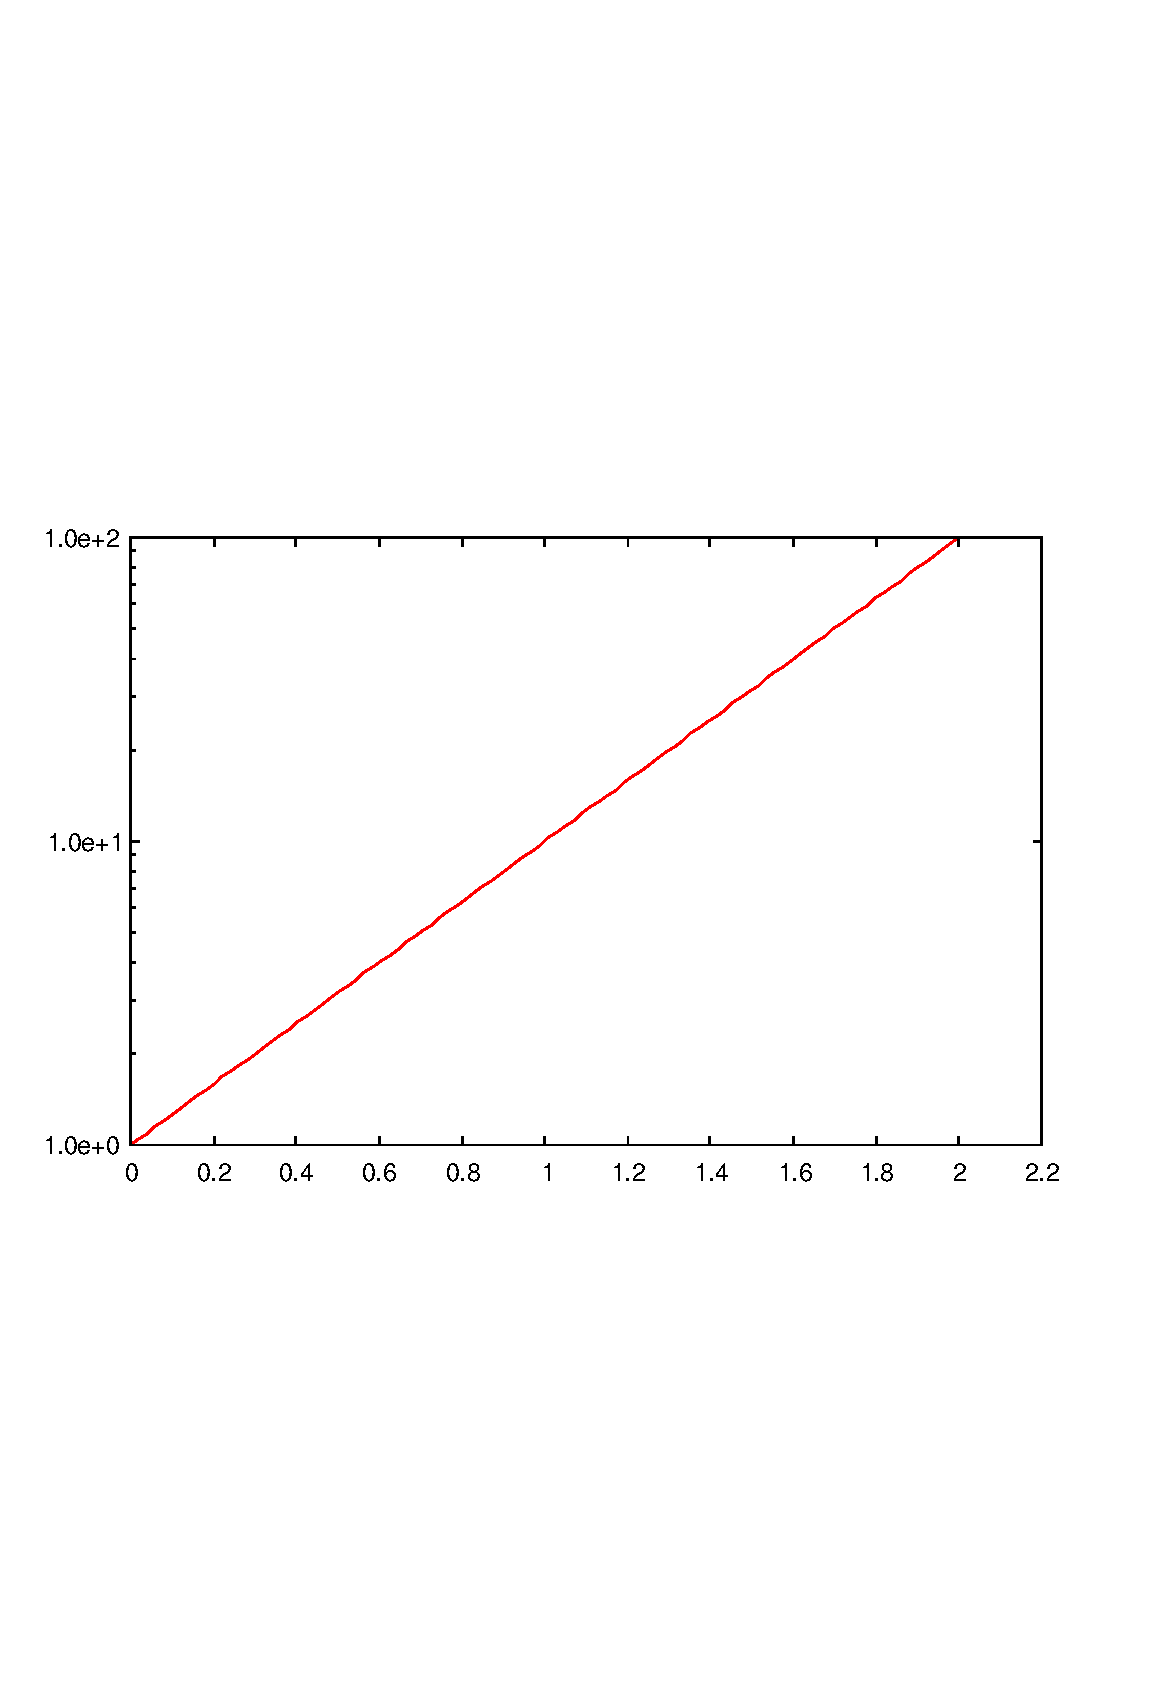
\includegraphics[width=12cm]{semilogy2}
\caption{semilogy2}
\end{DoxyImage}
 \hypertarget{handle_set}{}\section{S\-E\-T Set Object Property}\label{handle_set}
Section\-: \hyperlink{sec_handle}{Handle-\/\-Based Graphics} \hypertarget{vtkwidgets_vtkxyplotwidget_Usage}{}\subsection{Usage}\label{vtkwidgets_vtkxyplotwidget_Usage}
This function allows you to change the value associated with a property. The syntax for its use is \begin{DoxyVerb}  set(handle,property,value,property,value,...)
\end{DoxyVerb}
 where {\ttfamily property} is a string containing the name of the property, and {\ttfamily value} is the value for that property. The type of the variable {\ttfamily value} depends on the property being set. See the help for the properties to see what values you can set. \hypertarget{handle_sizefig}{}\section{S\-I\-Z\-E\-F\-I\-G Set Size of Figure}\label{handle_sizefig}
Section\-: \hyperlink{sec_handle}{Handle-\/\-Based Graphics} \hypertarget{vtkwidgets_vtkxyplotwidget_Usage}{}\subsection{Usage}\label{vtkwidgets_vtkxyplotwidget_Usage}
The {\ttfamily sizefig} function changes the size of the currently selected fig window. The general syntax for its use is \begin{DoxyVerb}   sizefig(width,height)
\end{DoxyVerb}
 where {\ttfamily width} and {\ttfamily height} are the dimensions of the fig window. \hypertarget{handle_subplot}{}\section{S\-U\-B\-P\-L\-O\-T Subplot Function}\label{handle_subplot}
Section\-: \hyperlink{sec_handle}{Handle-\/\-Based Graphics} \hypertarget{vtkwidgets_vtkxyplotwidget_Usage}{}\subsection{Usage}\label{vtkwidgets_vtkxyplotwidget_Usage}
This function divides the current figure into a 2-\/dimensional grid, each of which can contain a plot of some kind. The function has a number of syntaxes. The first version \begin{DoxyVerb}   subplot(row,col,num)
\end{DoxyVerb}
 which either activates subplot number {\ttfamily num}, or sets up a subplot grid of size {\ttfamily row x col}, and then activates {\ttfamily num}. You can also set up subplots that cover multiple grid elements \begin{DoxyVerb}   subplot(row,col,[vec])
\end{DoxyVerb}
 where {\ttfamily vec} is a set of indexes covered by the new subplot. Finally, as a shortcut, you can specify a string with three components \begin{DoxyVerb}   subplot('mnp')
\end{DoxyVerb}
 or using the alternate notation \begin{DoxyVerb}   subplot mnp
\end{DoxyVerb}
 where {\ttfamily m} is the number of rows, {\ttfamily n} is the number of columns and {\ttfamily p} is the index. You can also specify the location of the subplot explicitly using the syntax \begin{DoxyVerb}   subplot('position',[left bottom width height])
\end{DoxyVerb}
\hypertarget{variables_struct_Example}{}\subsection{Example}\label{variables_struct_Example}
Here is the use of {\ttfamily subplot} to set up a {\ttfamily 2 x 2} grid of plots


\begin{DoxyVerbInclude}
--> t = linspace(-pi,pi);
--> subplot(2,2,1)
--> plot(t,cos(t).*exp(-2*t));
--> subplot(2,2,2);
--> plot(t,cos(t*2).*exp(-2*t));
--> subplot(2,2,3);
--> plot(t,cos(t*3).*exp(-2*t));
--> subplot(2,2,4);
--> plot(t,cos(t*4).*exp(-2*t));
\end{DoxyVerbInclude}


 
\begin{DoxyImage}
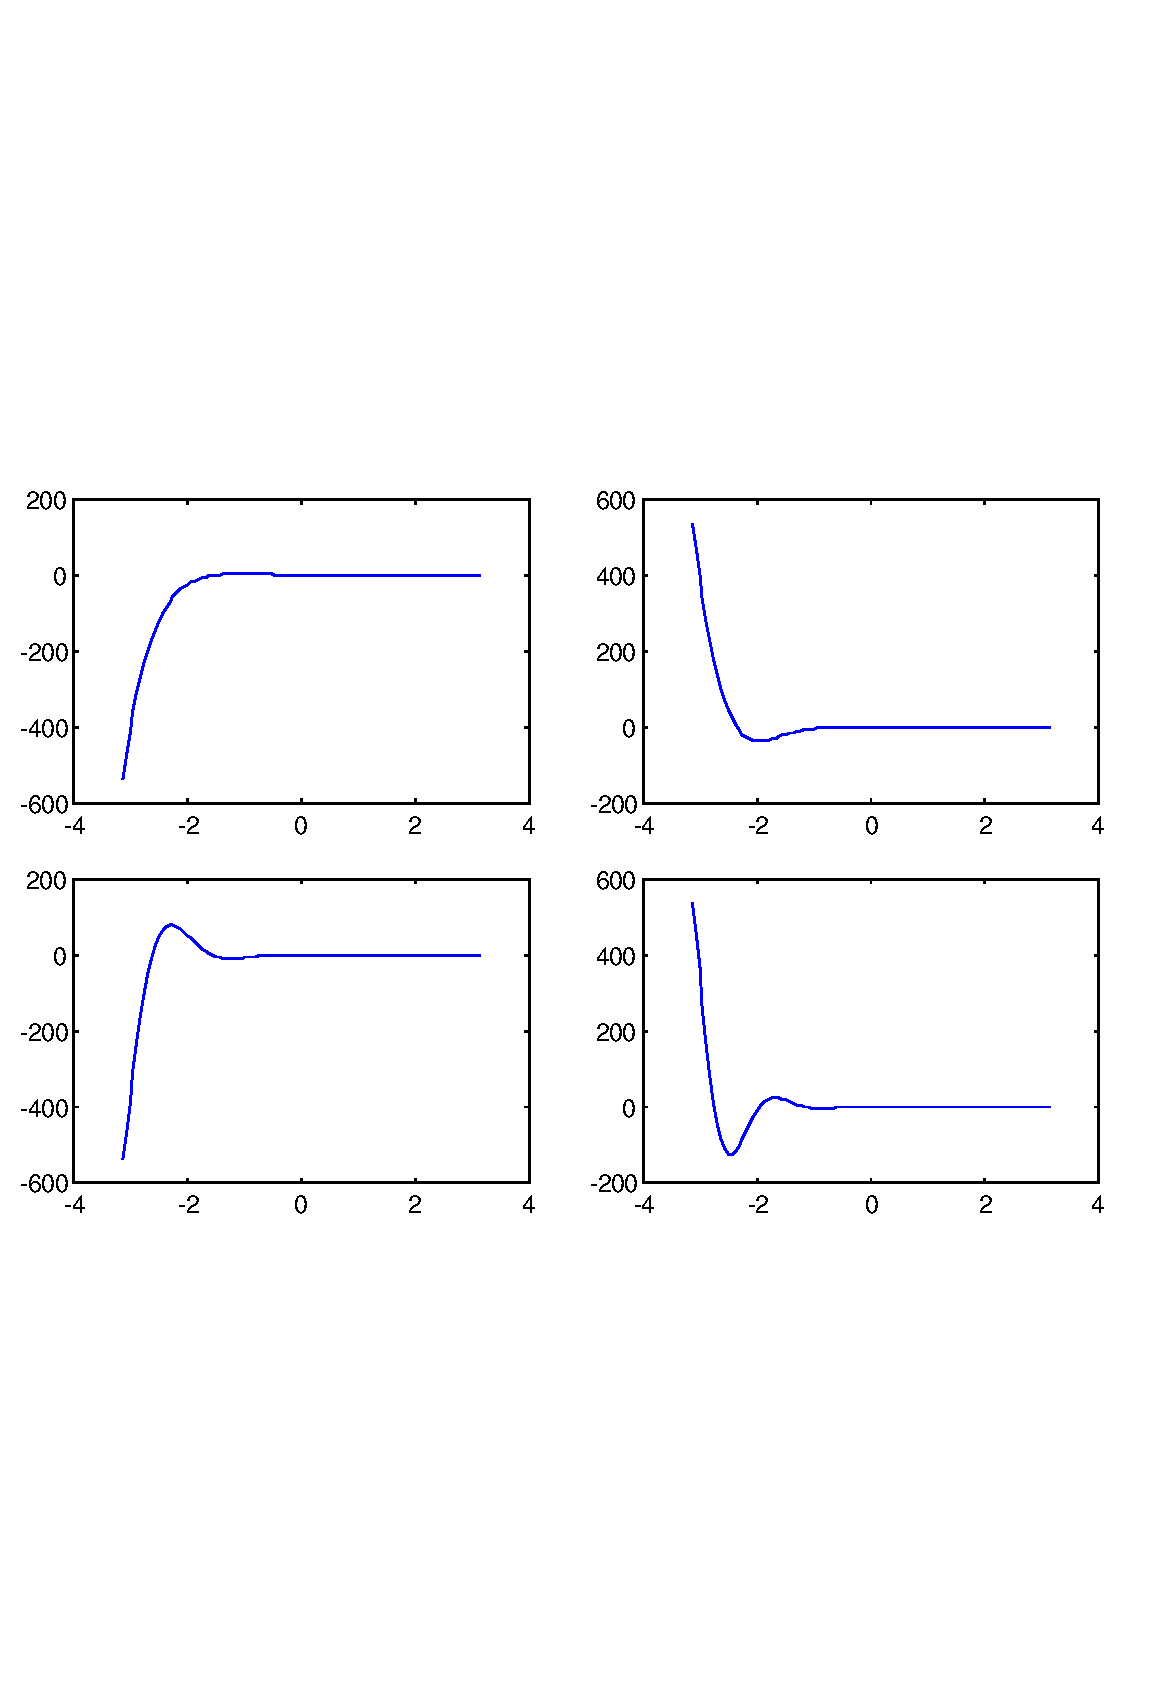
\includegraphics[width=12cm]{subplot1}
\caption{subplot1}
\end{DoxyImage}
 Here we use the second form of {\ttfamily subplot} to generate one subplot that is twice as large.


\begin{DoxyVerbInclude}
--> t = linspace(-pi,pi);
--> subplot(2,2,[1,2])
--> plot(t,cos(t).*exp(-2*t));
--> subplot(2,2,3);
--> plot(t,cos(t*3).*exp(-2*t));
--> subplot(2,2,4);
--> plot(t,cos(t*4).*exp(-2*t));
\end{DoxyVerbInclude}


 
\begin{DoxyImage}
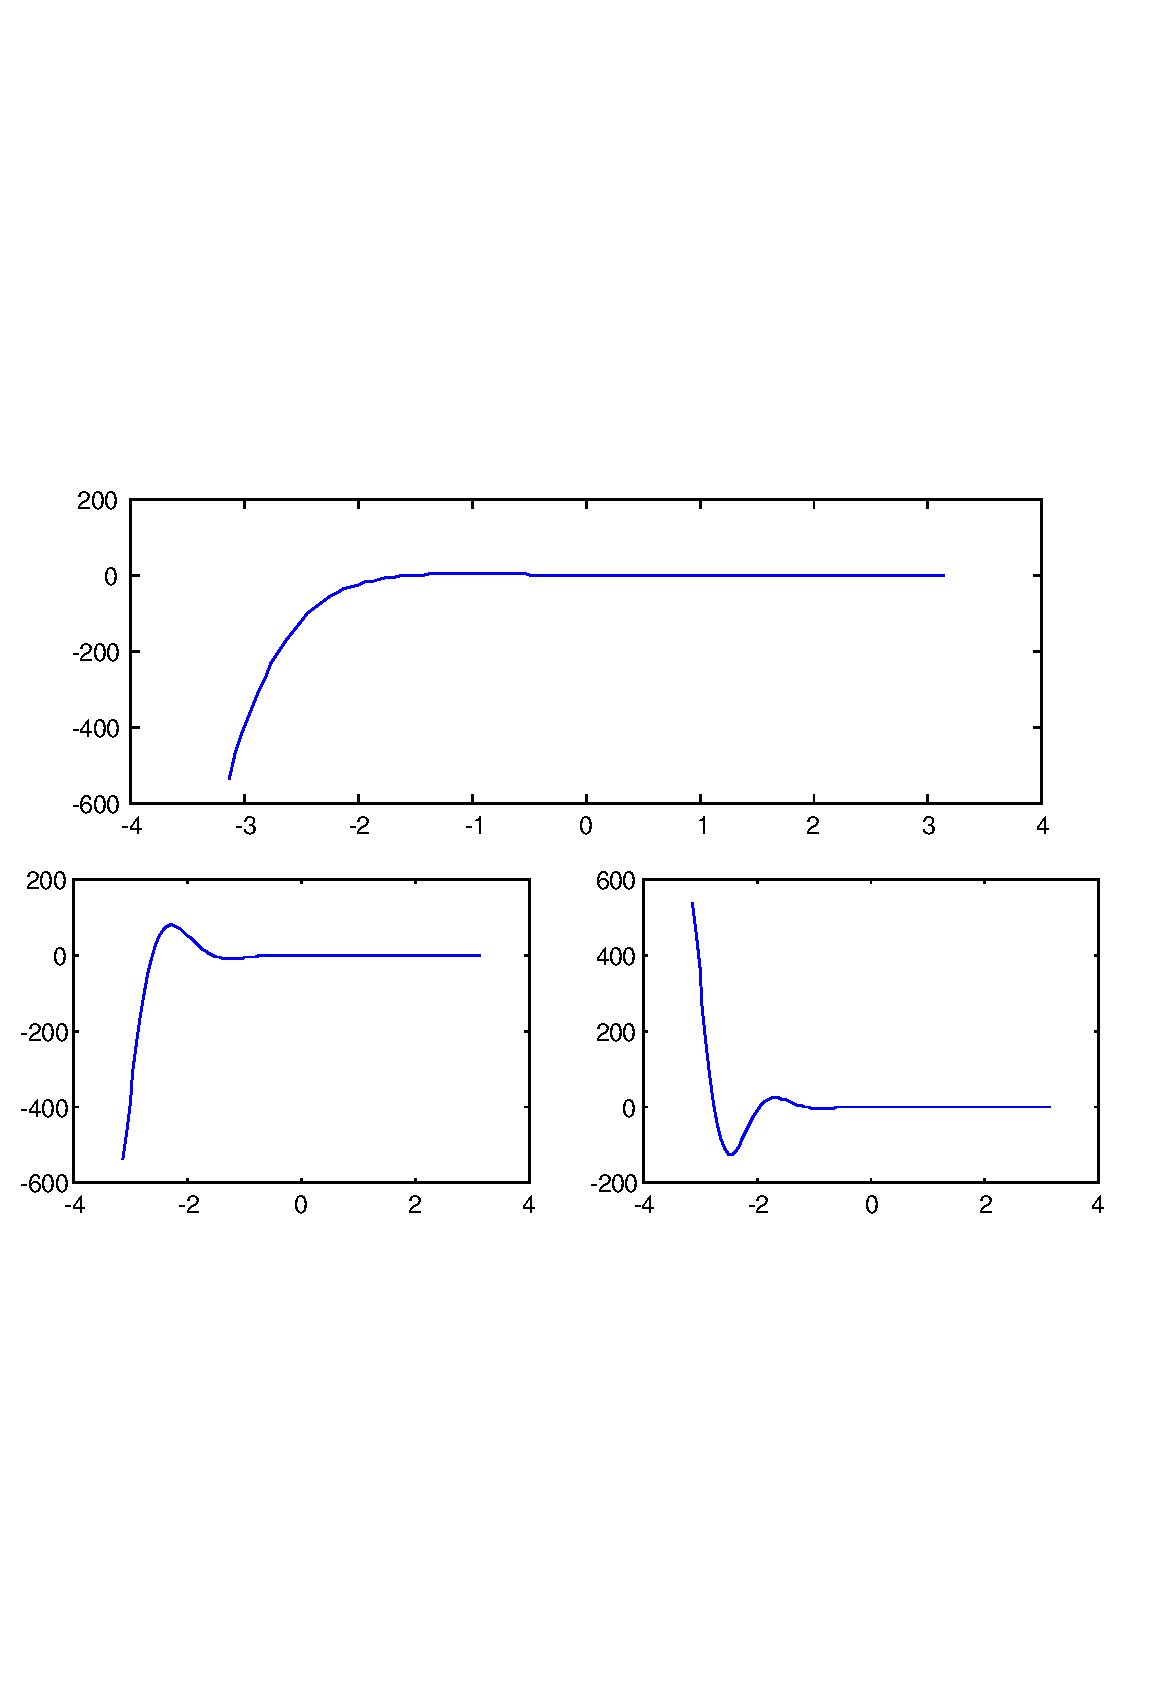
\includegraphics[width=12cm]{subplot2}
\caption{subplot2}
\end{DoxyImage}
 Note that the subplots can contain any handle graphics objects, not only simple plots.


\begin{DoxyVerbInclude}
--> t=0:(2*pi/100):(2*pi);
--> x=cos(t*2).*(2+sin(t*3)*.3);
--> y=sin(t*2).*(2+sin(t*3)*.3);
--> z=cos(t*3)*.3;
--> subplot(2,2,1)
--> plot(t,x);
--> subplot(2,2,2);
--> plot(t,y);
--> subplot(2,2,3);
--> plot(t,z);
--> subplot(2,2,4);
--> tubeplot(x,y,z,0.14*sin(t*5)+.29,t,10)
--> axis equal
--> view(3)
\end{DoxyVerbInclude}


 
\begin{DoxyImage}
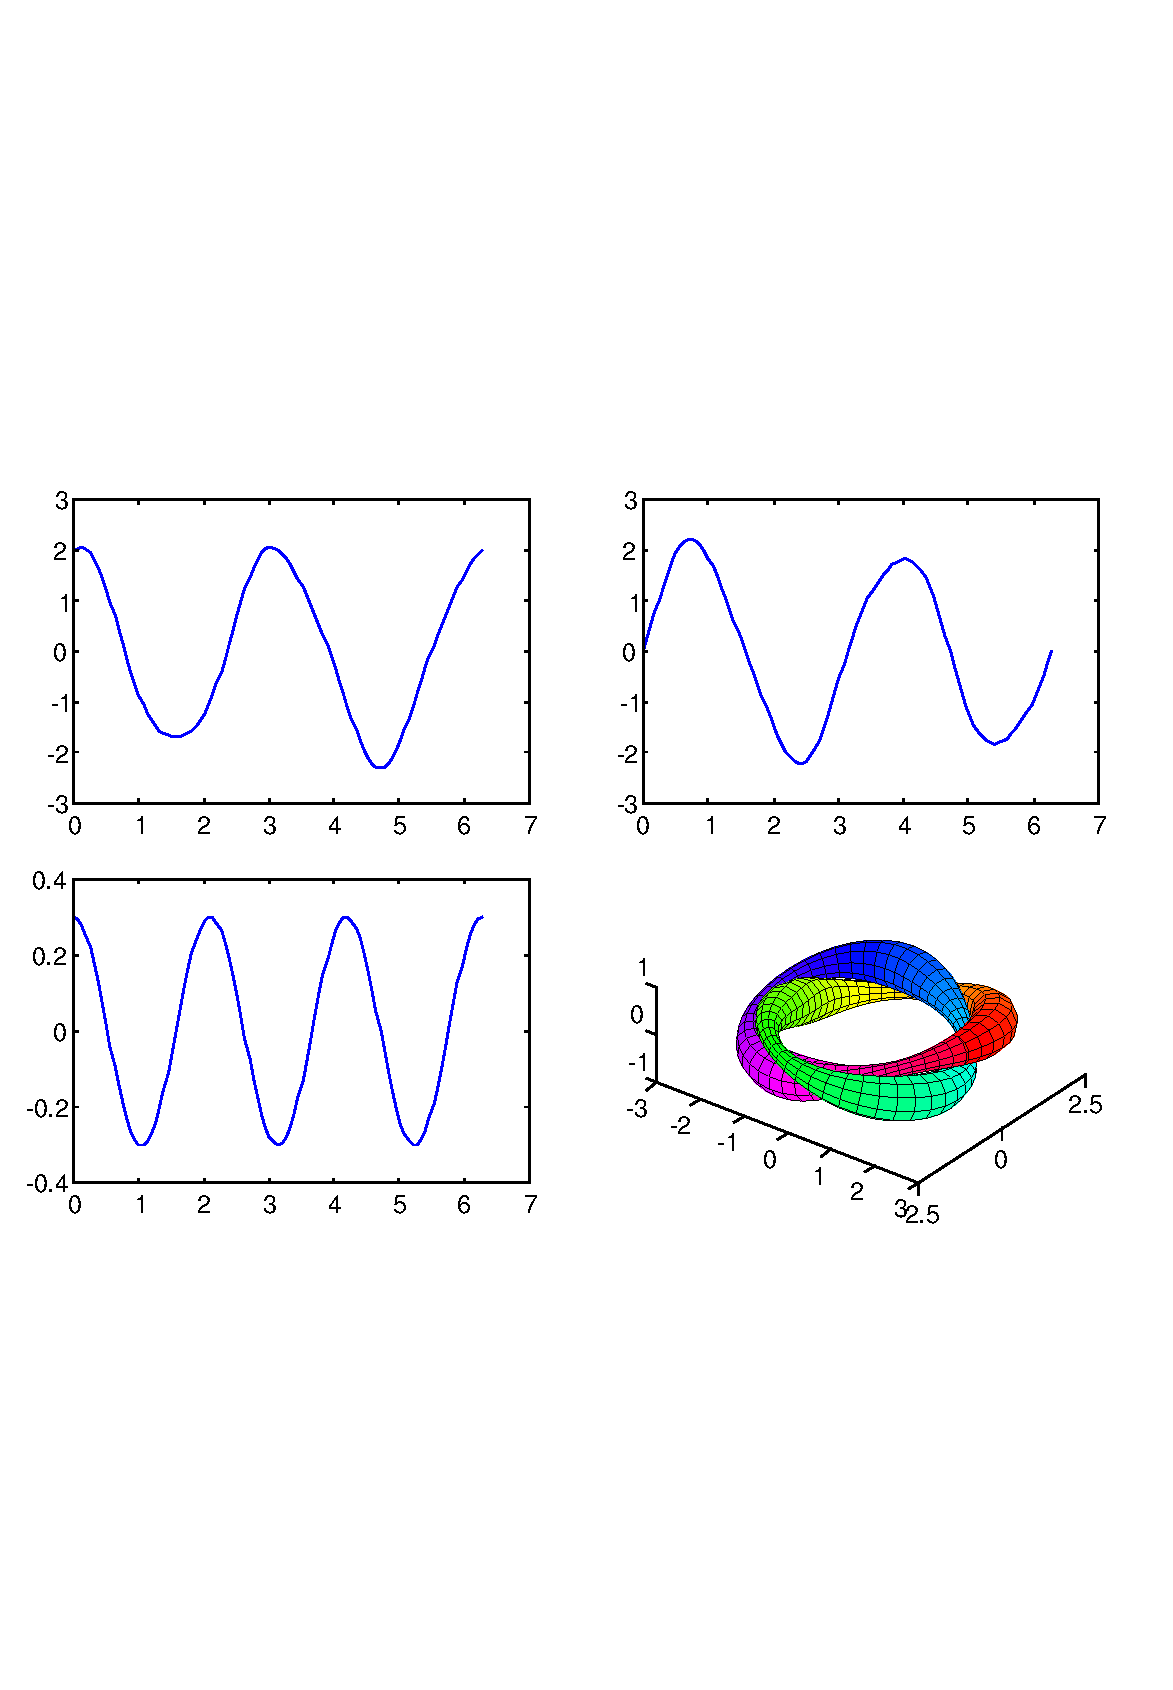
\includegraphics[width=12cm]{subplot3}
\caption{subplot3}
\end{DoxyImage}
 \hypertarget{handle_surf}{}\section{S\-U\-R\-F Surface Plot Function}\label{handle_surf}
Section\-: \hyperlink{sec_handle}{Handle-\/\-Based Graphics} \hypertarget{vtkwidgets_vtkxyplotwidget_Usage}{}\subsection{Usage}\label{vtkwidgets_vtkxyplotwidget_Usage}
This routine is used to create a surface plot of data. A surface plot is a 3\-D surface defined by the xyz coordinates of its vertices and optionally by the color at the vertices. The most general syntax for the {\ttfamily surf} function is \begin{DoxyVerb}  h = surf(X,Y,Z,C,properties...)
\end{DoxyVerb}
 Where {\ttfamily X} is a matrix or vector of {\ttfamily x} coordinates, {\ttfamily Y} is a matrix or vector of {\ttfamily y} coordinates, {\ttfamily Z} is a 2\-D matrix of coordinates, and {\ttfamily C} is a 2\-D matrix of color values (the colormap for the current fig is applied). In general, {\ttfamily X} and {\ttfamily Y} should be the same size as {\ttfamily Z}, but Free\-Mat will expand vectors to match the matrix if possible. If you want the color of the surface to be defined by the height of the surface, you can omit {\ttfamily C} \begin{DoxyVerb}  h = surf(X,Y,Z,properties...)
\end{DoxyVerb}
 in which case {\ttfamily C=Z}. You can also eliminate the {\ttfamily X} and {\ttfamily Y} matrices in the specification \begin{DoxyVerb}  h = surf(Z,properties)
\end{DoxyVerb}
 in which case they are set to {\ttfamily 1\-:size(\-Z,2)} and {\ttfamily 1\-:size(\-Y,2)} respectively. You can also specify a handle as the target of the {\ttfamily surf} command via \begin{DoxyVerb}  h = surf(handle,...)
\end{DoxyVerb}
 \hypertarget{variables_struct_Example}{}\subsection{Example}\label{variables_struct_Example}
Here we generate a surface specifying all four components.


\begin{DoxyVerbInclude}
--> x = repmat(linspace(-1,1),[100,1]);
--> y = x';
--> r = x.^2+y.^2;
--> z = exp(-r*3).*cos(5*r);
--> c = r;
--> surf(x,y,z,c)
--> axis equal
--> view(3)
\end{DoxyVerbInclude}


 
\begin{DoxyImage}
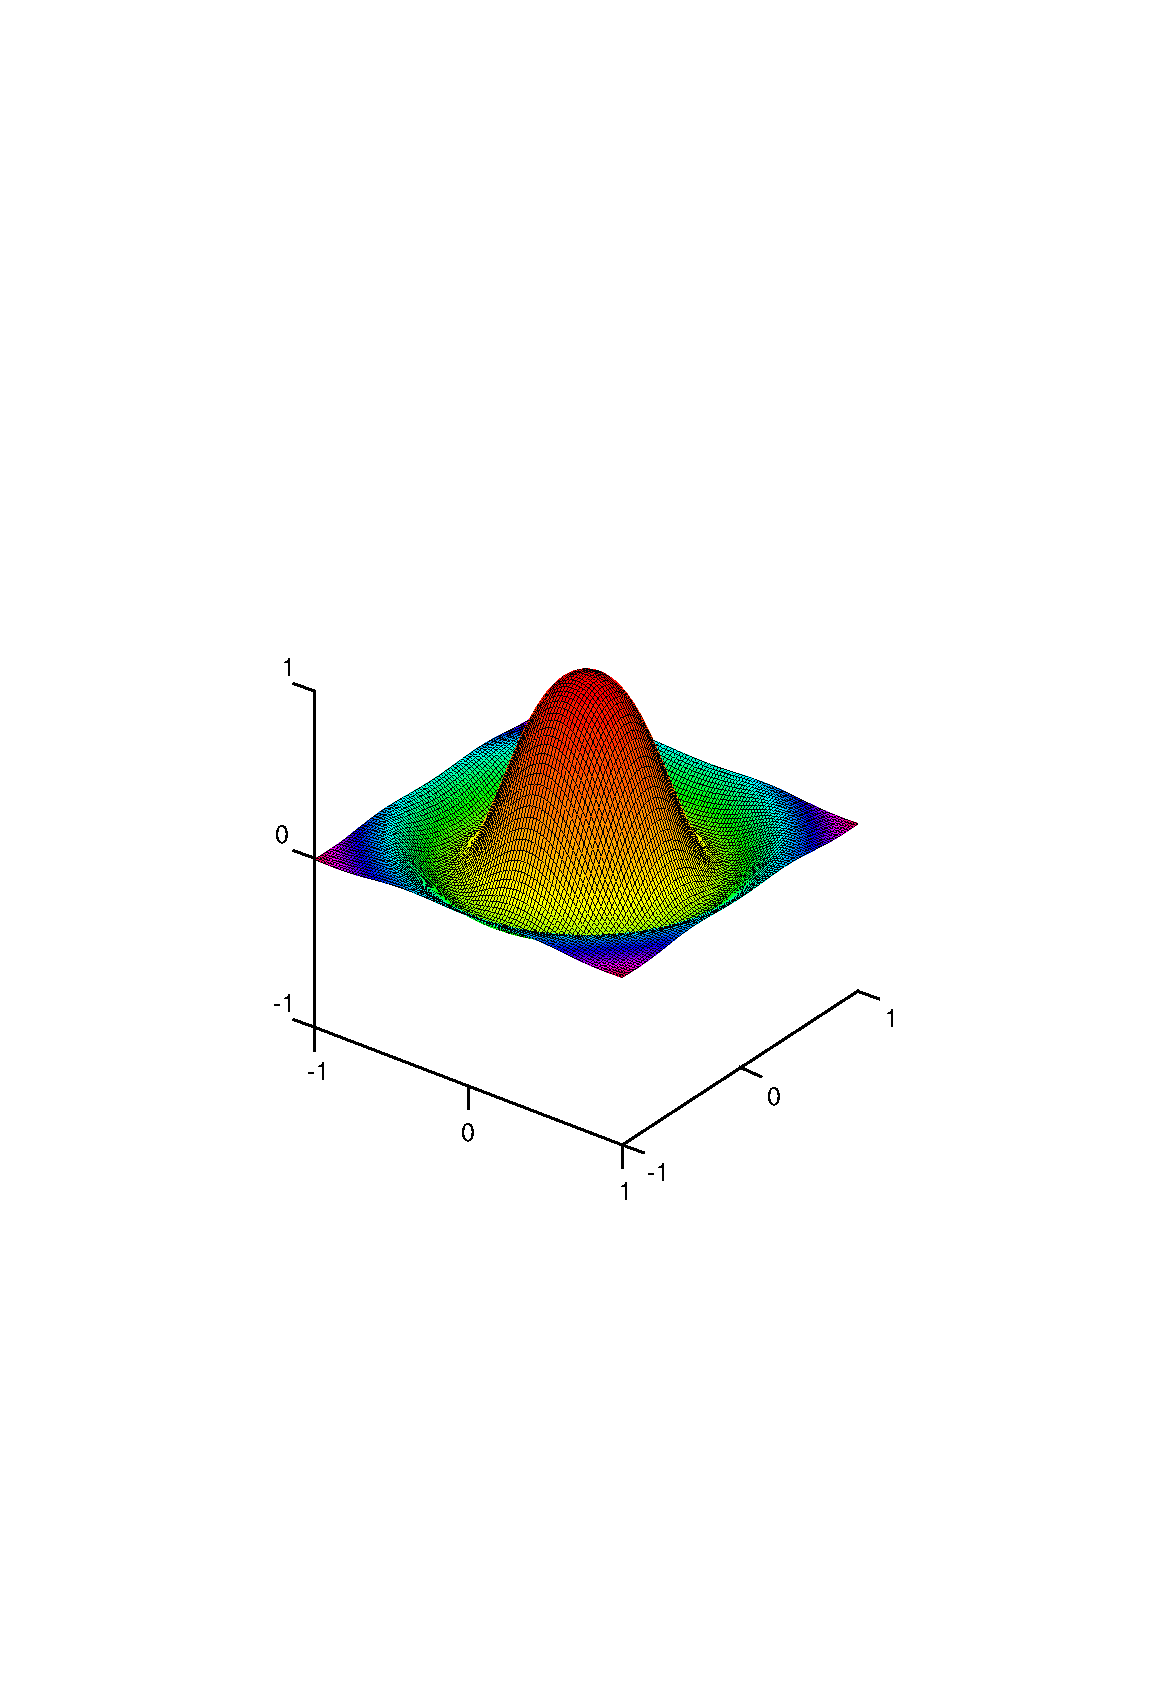
\includegraphics[width=12cm]{surf1}
\caption{surf1}
\end{DoxyImage}
 If we allow Free\-Mat to specify the color component, we see that the colorfield is the same as the height


\begin{DoxyVerbInclude}
--> surf(x,y,z)
--> axis equal
--> view(3)
\end{DoxyVerbInclude}


 
\begin{DoxyImage}
\includegraphics[width=12cm]{surf2}
\caption{surf2}
\end{DoxyImage}
 \hypertarget{handle_surfaceproperties}{}\section{S\-U\-R\-F\-A\-C\-E\-P\-R\-O\-P\-E\-R\-T\-I\-E\-S Surface Object Properties}\label{handle_surfaceproperties}
Section\-: \hyperlink{sec_handle}{Handle-\/\-Based Graphics} \hypertarget{vtkwidgets_vtkxyplotwidget_Usage}{}\subsection{Usage}\label{vtkwidgets_vtkxyplotwidget_Usage}
Below is a summary of the properties for the axis. 
\begin{DoxyItemize}
\item {\ttfamily alphadata} -\/ {\ttfamily vector} -\/ This is a vector that should contain as many elements as the surface data itself {\ttfamily cdata}, or a single scalar. For a single scalar, all values of the surface take on the same transparency. Otherwise, the transparency of each pixel is determined by the corresponding value from the {\ttfamily alphadata} vector.  
\item {\ttfamily alphadatamapping} -\/ {\ttfamily \{'scaled','direct','none'\}} -\/ For {\ttfamily none} mode (the default), no transparency is applied to the data. For {\ttfamily direct} mode, the vector {\ttfamily alphadata} contains values between @\mbox{[}0,M-\/1\mbox{]}$|$ where {\ttfamily M} is the length of the alpha map stored in the figure. For {\ttfamily scaled} mode, the {\ttfamily alim} vector for the figure is used to linearly rescale the alpha data prior to lookup in the alpha map.  
\item {\ttfamily ambientstrength} -\/ Not used.  
\item {\ttfamily backfacelighting} -\/ Not used.  
\item {\ttfamily cdata} -\/ {\ttfamily array} -\/ This is either a {\ttfamily M x N} array or an {\ttfamily M x N x 3} array. If the data is {\ttfamily M x N} the surface is a scalar surface (indexed mode), where the color associated with each surface pixel is computed using the colormap and the {\ttfamily cdatamapping} mode. If the data is {\ttfamily M x N x 3} the surface is assumed to be in R\-G\-B mode, and the colorpanes are taken directly from {\ttfamily cdata} (the colormap is ignored). Note that in this case, the data values must be between @\mbox{[}0,1\mbox{]}$|$ for each color channel and each point on the surface.  
\item {\ttfamily cdatamapping} -\/ {\ttfamily \{'scaled','direct'\}} -\/ For {\ttfamily scaled} (the default), the pixel values are scaled using the {\ttfamily clim} vector for the figure prior to looking up in the colormap. For {\ttfamily direct} mode, the pixel values must be in the range {\ttfamily \mbox{[}0,N-\/1} where {\ttfamily N} is the number of colors in the colormap.  
\item {\ttfamily children} -\/ Not used.  
\item {\ttfamily diffusestrength} -\/ Not used.  
\item {\ttfamily edgealpha} -\/ {\ttfamily \{'flat','interp','scalar'\}} -\/ Controls how the transparency is mapped for the edges of the surface.  
\item {\ttfamily edgecolor} -\/ {\ttfamily \{'flat','interp','none',colorspec\}} -\/ Specifies how the edges are colored. For {\ttfamily 'flat'} the edges are flat colored, meaning that the line segments that make up the edges are not shaded. The color for the line is determined by the first edge point it is connected to.  
\item {\ttfamily edgelighting} -\/ Not used.  
\item {\ttfamily facealpha} -\/ {\ttfamily \{'flat','interp','texturemap',scalar\}} -\/ Controls how the transparency of the faces of the surface are controlled. For flat shading, the faces are constant transparency. For interp mode, the faces are smoothly transparently mapped. If set to a scalar, all faces have the same transparency.  
\item {\ttfamily facecolor} -\/ {\ttfamily \{'none','flat','interp',colorspec\}} -\/ Controls how the faces are colored. For {\ttfamily 'none'} the faces are uncolored, and the surface appears as a mesh without hidden lines removed. For {\ttfamily 'flat'} the surface faces have a constant color. For {\ttfamily 'interp'} smooth shading is applied to the surface. And if a colorspec is provided, then the faces all have the same color.  
\item {\ttfamily facelighting} -\/ Not used.  
\item {\ttfamily linestyle} -\/ {\ttfamily \{'-\/','--','\-:','-\/.','none'\}} -\/ The style of the line used to draw the edges.  
\item {\ttfamily linewidth} -\/ {\ttfamily scalar} -\/ The width of the line used to draw the edges.  
\item {\ttfamily marker} -\/ {\ttfamily \{'+','o','$\ast$','.','x','square','s','diamond','d','$^\wedge$','v','$>$','$<$'\}} -\/ The marker for data points on the line. Some of these are redundant, as {\ttfamily 'square'} {\ttfamily 's'} are synonyms, and {\ttfamily 'diamond'} and {\ttfamily 'd'} are also synonyms.  
\item {\ttfamily markeredgecolor} -\/ {\ttfamily colorspec} -\/ The color used to draw the marker. For some of the markers (circle, square, etc.) there are two colors used to draw the marker. This property controls the edge color (which for unfilled markers) is the primary color of the marker.  
\item {\ttfamily markerfacecolor} -\/ {\ttfamily colorspec} -\/ The color used to fill the marker. For some of the markers (circle, square, etc.) there are two colors used to fill the marker.  
\item {\ttfamily markersize} -\/ {\ttfamily scalar} -\/ Control the size of the marker. Defaults to 6, which is effectively the radius (in pixels) of the markers.  
\item {\ttfamily meshstyle} -\/ {\ttfamily \{'both','rows','cols\}} -\/ This property controls how the mesh is drawn for the surface. For {\ttfamily rows} and {\ttfamily cols} modes, only one set of edges is drawn.  
\item {\ttfamily normalmode} -\/ Not used.  
\item {\ttfamily parent} -\/ {\ttfamily handle} -\/ The axis containing the surface.  
\item {\ttfamily specularcolorreflectance} -\/ Not used.  
\item {\ttfamily specularexponent} -\/ Not used.  
\item {\ttfamily specularstrength} -\/ Not used.  
\item {\ttfamily tag} -\/ {\ttfamily string} -\/ You can set this to any string you want.  
\item {\ttfamily type} -\/ {\ttfamily string} -\/ Set to the string {\ttfamily 'surface'}.  
\item {\ttfamily userdata} -\/ {\ttfamily array} -\/ Available to store any variable you want in the handle object.  
\item {\ttfamily vertexnormals} -\/ Not used.  
\item {\ttfamily xdata} -\/ {\ttfamily array} -\/ Must be a numeric array of size {\ttfamily M x N} which contains the x location of each point in the defined surface. Must be the same size as {\ttfamily ydata} and {\ttfamily zdata}. Alternately, you can specify an array of size {\ttfamily 1 x N} in which case Free\-Mat replicates the vector to fill out an {\ttfamily M x N} matrix.  
\item {\ttfamily xdatamode} -\/ {\ttfamily \{'auto','manual'\}} -\/ When set to {\ttfamily auto} then Free\-Mat will automatically generate the x coordinates.  
\item {\ttfamily ydata} -\/ {\ttfamily array} -\/ Must be a numeric array of size {\ttfamily M x N} which contains the y location of each point in the defined surface. Must be the same size as {\ttfamily xdata} and {\ttfamily zdata}. Alternately, you can specify an array of size {\ttfamily M x 1} in which case Free\-Mat replicates the vector to fill out an {\ttfamily M x N} matrix.  
\item {\ttfamily ydatamode} -\/ {\ttfamily \{'auto','manual'\}} -\/ When set to {\ttfamily auto} then Free\-Mat will automatically generate the y coordinates.  
\item {\ttfamily zdata} -\/ {\ttfamily array} -\/ Must be a numeric array of size {\ttfamily M x N} which contains the y location of each point in the defined surface. Must be the same size as {\ttfamily xdata} and {\ttfamily ydata}.  
\item {\ttfamily visible} -\/ {\ttfamily \{'on','off'\}} -\/ Controls whether the surface is visible or not.  
\end{DoxyItemize}\hypertarget{handle_text}{}\section{T\-E\-X\-T Add Text Label to Plot}\label{handle_text}
Section\-: \hyperlink{sec_handle}{Handle-\/\-Based Graphics} \hypertarget{vtkwidgets_vtkxyplotwidget_Usage}{}\subsection{Usage}\label{vtkwidgets_vtkxyplotwidget_Usage}
Adds a text label to the currently active plot. The general syntax for it is use is either \begin{DoxyVerb}   text(x,y,'label')
\end{DoxyVerb}
 where {\ttfamily x} and {\ttfamily y} are both vectors of the same length, in which case the text {\ttfamily 'label'} is added to the current plot at each of the coordinates {\ttfamily x(i),y(i)} (using the current axis to map these to screen coordinates). The second form supplies a cell-\/array of strings as the second argument, and allows you to place many labels simultaneously \begin{DoxyVerb}   text(x,y,{'label1','label2',....})
\end{DoxyVerb}
 where the number of elements in the cell array must match the size of vectors {\ttfamily x} and {\ttfamily y}. You can also specify properties for the labels via \begin{DoxyVerb}   handles = text(x,y,{labels},properties...)
\end{DoxyVerb}
 \hypertarget{variables_struct_Example}{}\subsection{Example}\label{variables_struct_Example}
Here is an example of a few labels being added to a random plot\-:


\begin{DoxyVerbInclude}
--> plot(rand(1,4))
--> text([2,3],[0.5,0.5],{'hello','there'})
\end{DoxyVerbInclude}


 
\begin{DoxyImage}
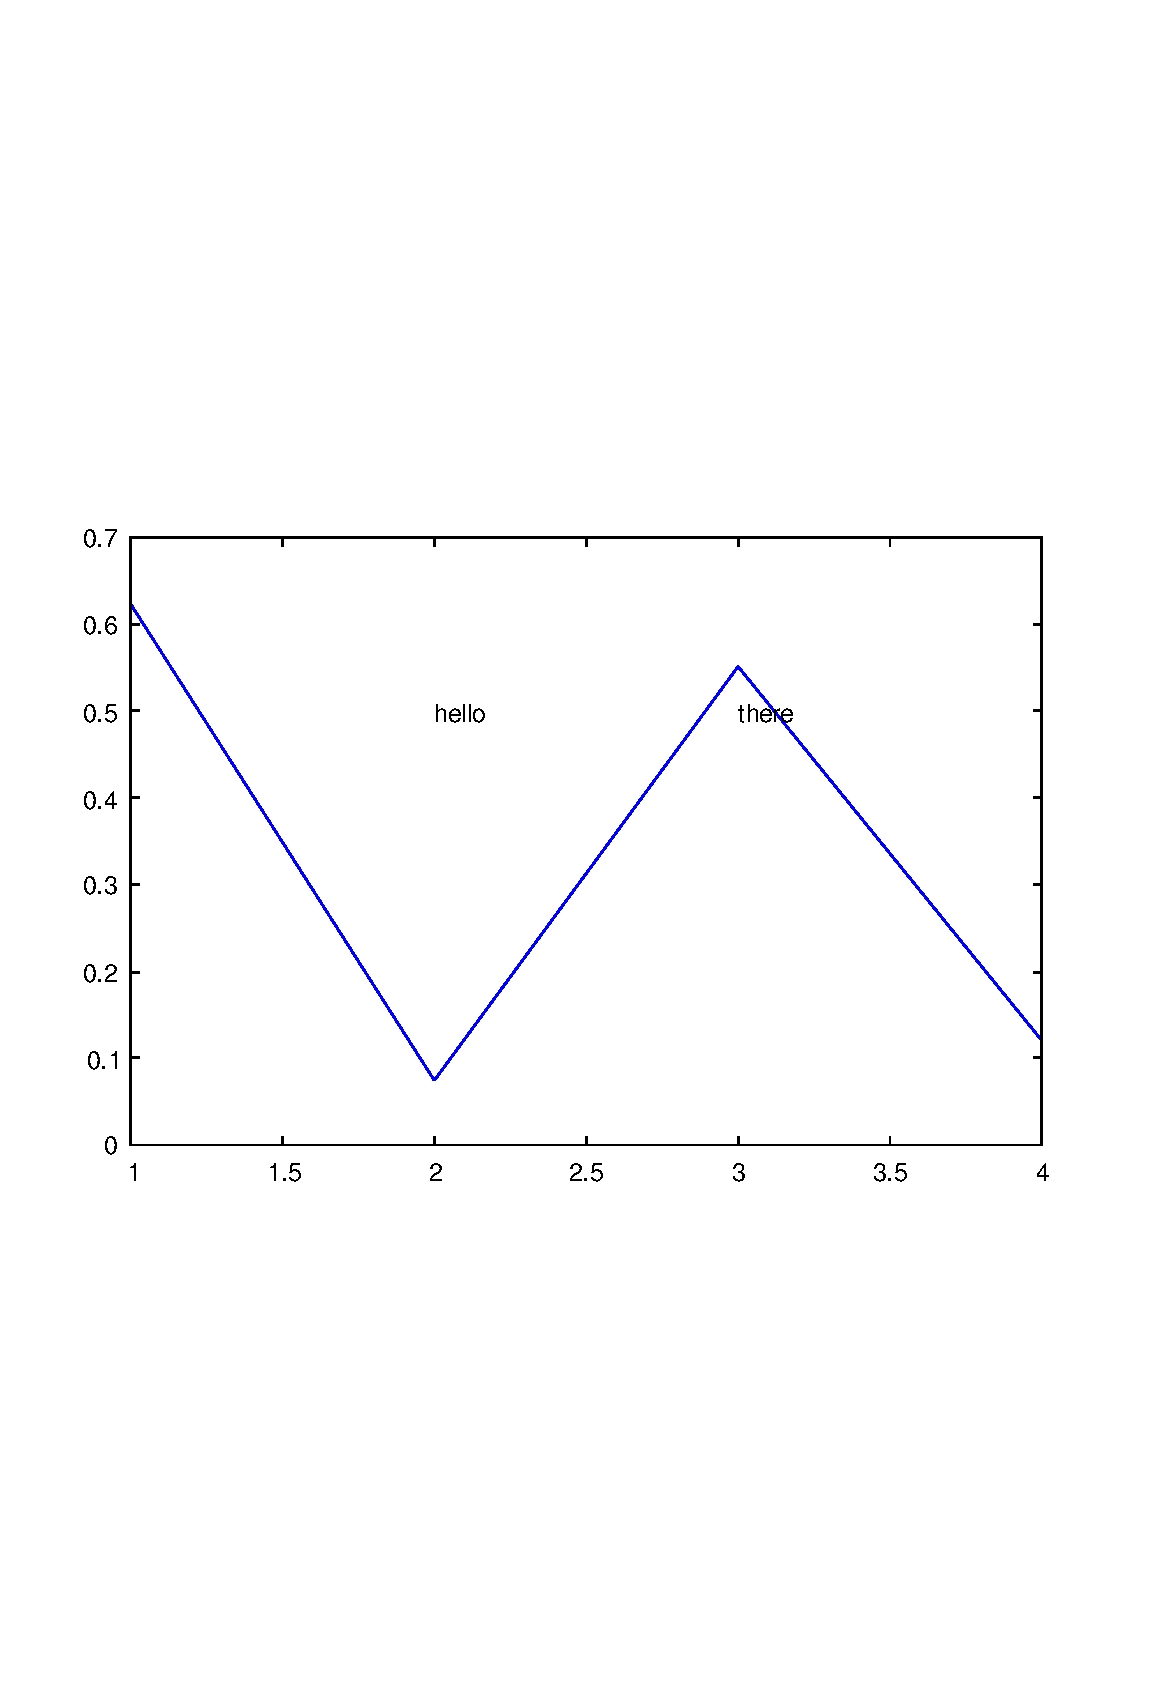
\includegraphics[width=12cm]{text1}
\caption{text1}
\end{DoxyImage}
 Here is the same example, but with larger labels\-:


\begin{DoxyVerbInclude}
--> plot(rand(1,4))
--> text([2,3],[0.5,0.5],{'hello','there'},'fontsize',20)
\end{DoxyVerbInclude}


 
\begin{DoxyImage}
\includegraphics[width=12cm]{text2}
\caption{text2}
\end{DoxyImage}
 \hypertarget{handle_textproperties}{}\section{T\-E\-X\-T\-P\-R\-O\-P\-E\-R\-T\-I\-E\-S Text Object Properties}\label{handle_textproperties}
Section\-: \hyperlink{sec_handle}{Handle-\/\-Based Graphics} \hypertarget{vtkwidgets_vtkxyplotwidget_Usage}{}\subsection{Usage}\label{vtkwidgets_vtkxyplotwidget_Usage}
Below is a summary of the properties for a text object. 
\begin{DoxyItemize}
\item {\ttfamily boundingbox} -\/ {\ttfamily four vector} -\/ The size of the bounding box containing the text (in pixels). May contain negative values if the text is slanted.  
\item {\ttfamily children} -\/ Not used.  
\item {\ttfamily string} -\/ {\ttfamily string} -\/ The text contained in the label.  
\item {\ttfamily extent} -\/ Not used.  
\item {\ttfamily horizontalalignment} -\/ {\ttfamily \{'left','center','right'\}} -\/ Controls the alignment of the text relative to the specified position point.  
\item {\ttfamily position} -\/ {\ttfamily three vector} -\/ The position of the label in axis coordinates.  
\item {\ttfamily rotation} -\/ {\ttfamily scalar} -\/ The rotation angle (in degrees) of the label.  
\item {\ttfamily units} -\/ Not used.  
\item {\ttfamily verticalalignment} -\/ {\ttfamily \{'top','bottom','middle'\}} -\/ Controls the alignment fo the text relative to the specified position point in the vertical position.  
\item {\ttfamily backgroundcolor} -\/ {\ttfamily colorspec} -\/ The color used to fill in the background rectangle for the label. Normally this is {\ttfamily none}.  
\item {\ttfamily edgecolor} -\/ {\ttfamily colorspec} -\/ The color used to draw the bounding rectangle for the label. Normally this is {\ttfamily none}.  
\item {\ttfamily linewidth} -\/ {\ttfamily scalar} -\/ The width of the line used to draw the border.  
\item {\ttfamily linestyle} -\/ {\ttfamily \{'-\/','--','\-:','-\/.','none'\}} -\/ The style of the line used to draw the border.  
\item {\ttfamily margin} -\/ {\ttfamily scalar} -\/ The amount of spacing to place around the text as padding when drawing the rectangle.  
\item {\ttfamily fontangle} -\/ {\ttfamily \{'normal','italic','oblique'\}} -\/ The angle of the fonts used for the labels.  
\item {\ttfamily fontsize} -\/ {\ttfamily scalar} -\/ The size of fonts used for the text.  
\item {\ttfamily fontunits} -\/ Not used.  
\item {\ttfamily fontweight} -\/ {\ttfamily \{'normal','bold','light','demi'\}} -\/ The weight of the font used for the label  
\item {\ttfamily visible} -\/ {\ttfamily \{'on','off'\}} -\/ Controls visibility of the the line.  
\item {\ttfamily color} -\/ {\ttfamily colorspec} -\/ The color of the text of the label.  
\item {\ttfamily children} -\/ Not used.  
\item {\ttfamily parent} -\/ The handle of the axis that owns this label.  
\item {\ttfamily tag} -\/ {\ttfamily string} -\/ A string that can be used to tag the object.  
\item {\ttfamily type} -\/ {\ttfamily string} -\/ Returns the string {\ttfamily 'text'}.  
\item {\ttfamily userdata} -\/ {\ttfamily array} -\/ Available to store any variable you want in the handle object.  
\end{DoxyItemize}\hypertarget{handle_title}{}\section{T\-I\-T\-L\-E Plot Title Function}\label{handle_title}
Section\-: \hyperlink{sec_handle}{Handle-\/\-Based Graphics} \hypertarget{vtkwidgets_vtkxyplotwidget_Usage}{}\subsection{Usage}\label{vtkwidgets_vtkxyplotwidget_Usage}
This command adds a title to the plot. The general syntax for its use is \begin{DoxyVerb}  title('label')
\end{DoxyVerb}
 or in the alternate form \begin{DoxyVerb}  title 'label'
\end{DoxyVerb}
 or simply \begin{DoxyVerb}  title label
\end{DoxyVerb}
 Here {\ttfamily label} is a string variable. You can also specify properties for the label, and a handle to serve as a target for the operation \begin{DoxyVerb}  title(handle,'label',properties...)
\end{DoxyVerb}
 \hypertarget{variables_struct_Example}{}\subsection{Example}\label{variables_struct_Example}
Here is an example of a simple plot with a title.


\begin{DoxyVerbInclude}
--> x = linspace(-1,1);
--> y = cos(2*pi*x);
--> plot(x,y,'r-');
--> title('cost over time');
\end{DoxyVerbInclude}


which results in the following plot.  
\begin{DoxyImage}
\includegraphics[width=12cm]{title1}
\caption{title1}
\end{DoxyImage}
 We now increase the size of the font using the properties of the {\ttfamily label}


\begin{DoxyVerbInclude}
--> title('cost over time','fontsize',20);
\end{DoxyVerbInclude}


 
\begin{DoxyImage}
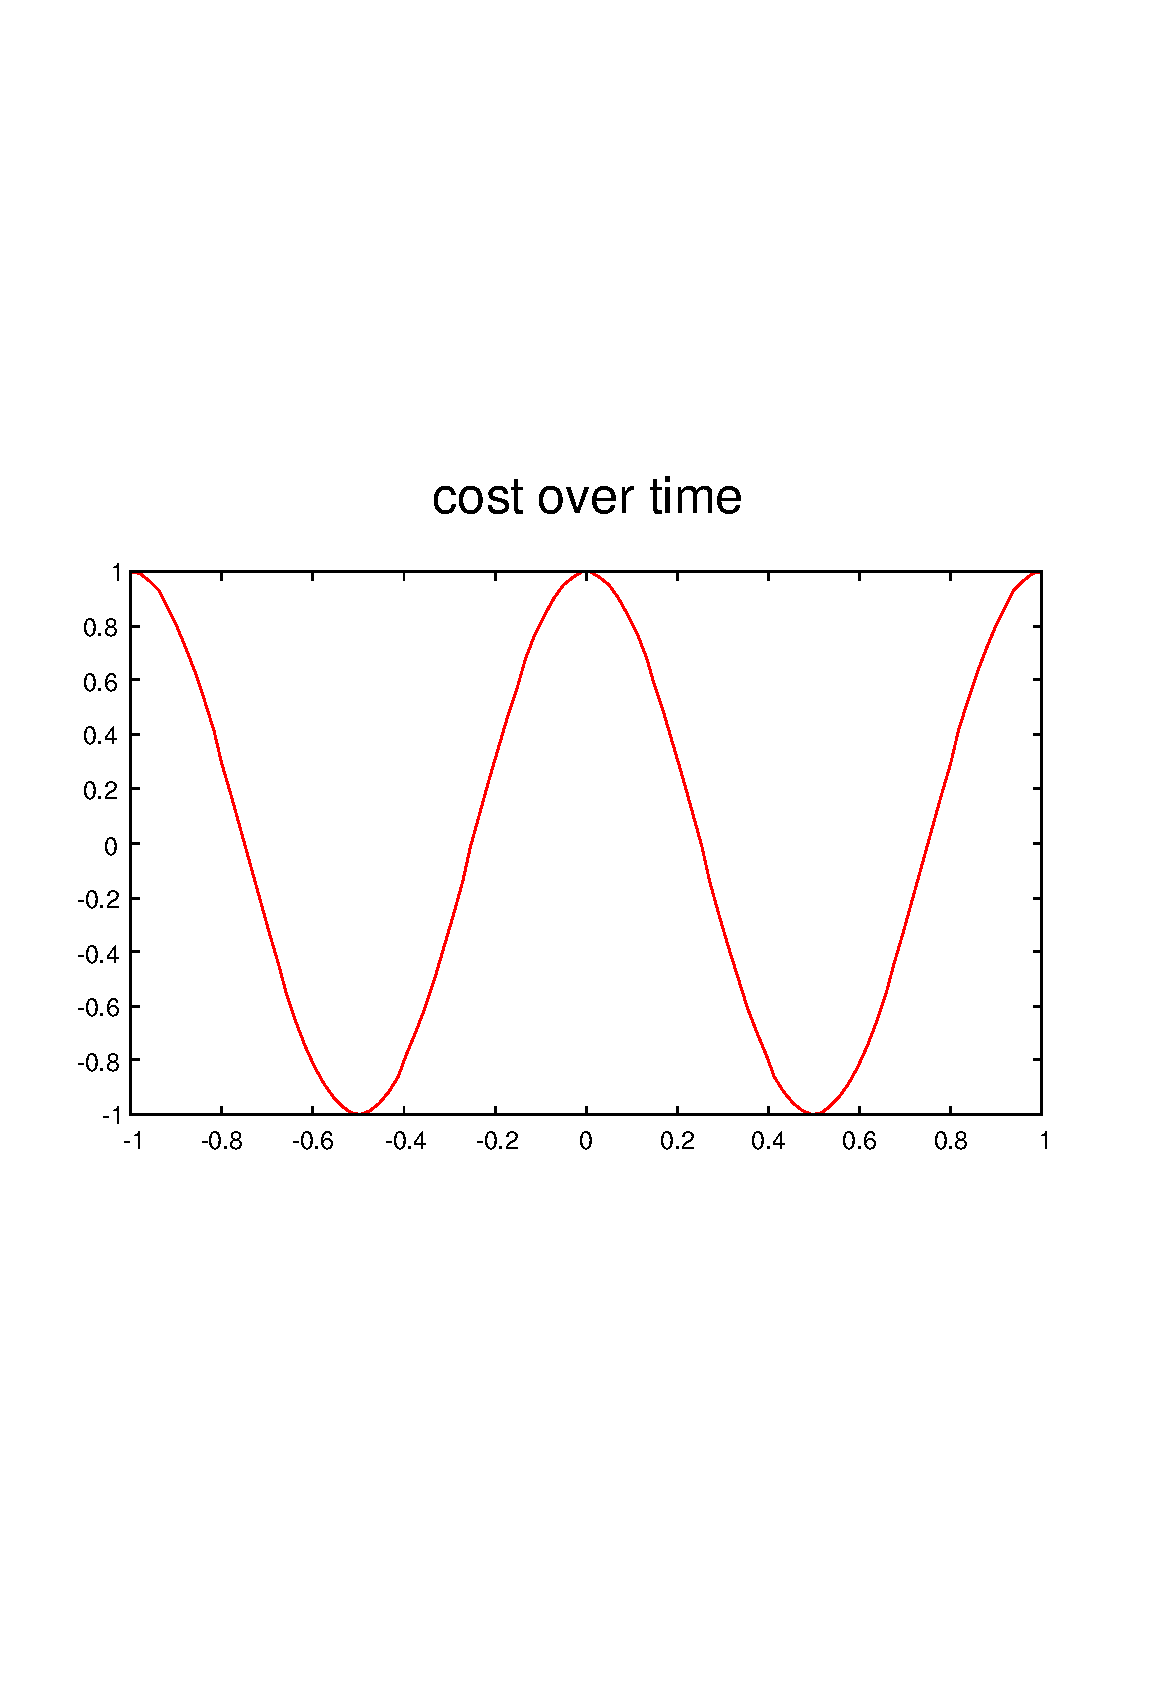
\includegraphics[width=12cm]{title2}
\caption{title2}
\end{DoxyImage}
 \hypertarget{handle_tubeplot}{}\section{T\-U\-B\-E\-P\-L\-O\-T Creates a Tubeplot}\label{handle_tubeplot}
Section\-: \hyperlink{sec_handle}{Handle-\/\-Based Graphics} \hypertarget{vtkwidgets_vtkxyplotwidget_Usage}{}\subsection{Usage}\label{vtkwidgets_vtkxyplotwidget_Usage}
This {\ttfamily tubeplot} function is from the tubeplot package written by Anders Sandberg. The simplest syntax for the {\ttfamily tubeplot} routine is \begin{DoxyVerb}    tubeplot(x,y,z)
\end{DoxyVerb}
 plots the basic tube with radius 1, where {\ttfamily x,y,z} are vectors that describe the tube. If the radius of the tube is to be varied, use the second form \begin{DoxyVerb}    tubeplot(x,y,z,r) 
\end{DoxyVerb}
 which plots the basic tube with variable radius r (either a vector or a scalar value). The third form allows you to specify the coloring using a vector of values\-: \begin{DoxyVerb}    tubeplot(x,y,z,r,v)
\end{DoxyVerb}
 where the coloring is now dependent on the values in the vector {\ttfamily v}. If you want to create a tube plot with a greater degree of tangential subdivisions (i.\-e., the tube is more circular, use the form \begin{DoxyVerb}    tubeplot(x,y,z,r,v,s)
\end{DoxyVerb}
 where {\ttfamily s} is the number of tangential subdivisions (default is 6) You can also use {\ttfamily tubeplot} to calculate matrices to feed to {\ttfamily mesh} and {\ttfamily surf}. \begin{DoxyVerb}    [X,Y,Z]=tubeplot(x,y,z)
\end{DoxyVerb}
 returns {\ttfamily N x 3} matrices suitable for mesh or surf.

Note that the tube may pinch at points where the normal and binormal misbehaves. It is suitable for general space curves, not ones that contain straight sections. Normally the tube is calculated using the Frenet frame, making the tube minimally twisted except at inflexion points.

To deal with this problem there is an alternative frame\-: \begin{DoxyVerb}    tubeplot(x,y,z,r,v,s,vec)
\end{DoxyVerb}
 calculates the tube by setting the normal to the cross product of the tangent and the vector vec. If it is chosen so that it is always far from the tangent vector the frame will not twist unduly. \hypertarget{variables_struct_Example}{}\subsection{Example}\label{variables_struct_Example}
Here is an example of a {\ttfamily tubeplot}.


\begin{DoxyVerbInclude}
--> t=0:(2*pi/100):(2*pi);
--> x=cos(t*2).*(2+sin(t*3)*.3);
--> y=sin(t*2).*(2+sin(t*3)*.3);
--> z=cos(t*3)*.3;
--> tubeplot(x,y,z,0.14*sin(t*5)+.29,t,10);
\end{DoxyVerbInclude}


 
\begin{DoxyImage}
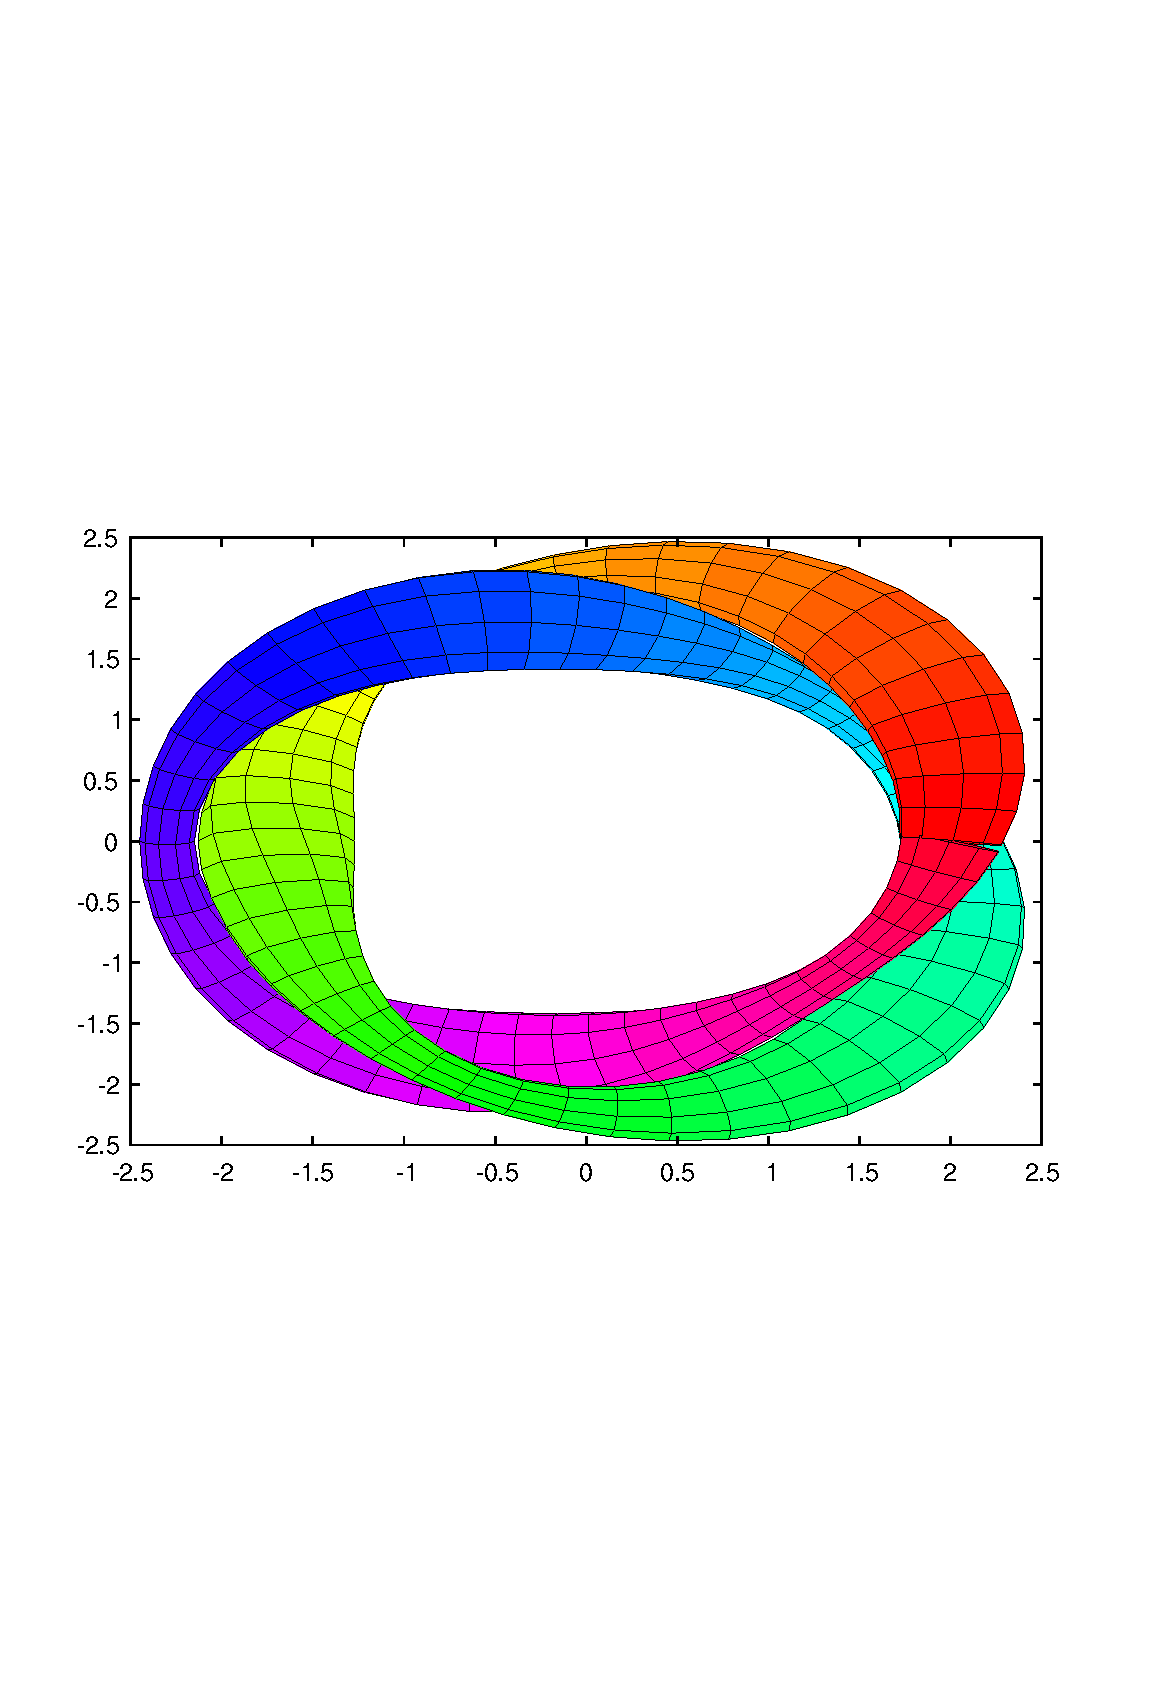
\includegraphics[width=12cm]{tubeplot1}
\caption{tubeplot1}
\end{DoxyImage}


Written by Anders Sandberg, \href{mailto:asa@nada.kth.se}{\tt asa@nada.\-kth.\-se}, 2005 Website says the package is free for anybody to use. www.\-nada.\-kth.\-se/$\sim$asa/\-Ray/\-Tubeplot/tubeplot.html \hypertarget{handle_uicontrol}{}\section{U\-I\-C\-O\-N\-T\-R\-O\-L Create a U\-I Control object}\label{handle_uicontrol}
Section\-: \hyperlink{sec_handle}{Handle-\/\-Based Graphics} \hypertarget{vtkwidgets_vtkxyplotwidget_Usage}{}\subsection{Usage}\label{vtkwidgets_vtkxyplotwidget_Usage}
Creates a U\-I control object and parents it to the current figure. The syntax for its use is \begin{DoxyVerb}  handle = uicontrol(property,value,property,value,...)
\end{DoxyVerb}
 where {\ttfamily property} and {\ttfamily value} are set. The handle I\-D for the resulting object is returned. It is automatically added to the children of the current figure. \hypertarget{handle_uicontrolproperties}{}\section{U\-I\-C\-O\-N\-T\-R\-O\-L\-P\-R\-O\-P\-E\-R\-T\-I\-E\-S U\-I Control Properties}\label{handle_uicontrolproperties}
Section\-: \hyperlink{sec_handle}{Handle-\/\-Based Graphics} \hypertarget{vtkwidgets_vtkxyplotwidget_Usage}{}\subsection{Usage}\label{vtkwidgets_vtkxyplotwidget_Usage}
Below is a summary of the properties for user interface controls. 
\begin{DoxyItemize}
\item {\ttfamily backgroundcolor} -\/ {\ttfamily colorspec} -\/ The background color for the widget.  
\item {\ttfamily busyaction} -\/ Not used.  
\item {\ttfamily buttondownfcn} -\/ Not used.  
\item {\ttfamily callback} -\/ {\ttfamily string} -\/ the callback to execute when the G\-U\-I control does its action. Clicking a button or moving a scroller will cause the callback to be executed. Also, pressing enter in a text box causes the callback to be executed.  
\item {\ttfamily cdata} -\/ an {\ttfamily M x N x 3} array that represents an R\-G\-B image to use as the truecolor image displayed on push bottons or toggle buttons. The values must be between 0 and 1.  
\item {\ttfamily children} -\/ Not used.  
\item {\ttfamily createfcn} -\/ Not used.  
\item {\ttfamily deletefcn} -\/ Not used;  
\item {\ttfamily enable} -\/ {\ttfamily \{'on','inactive','off'\}} -\/ For {\ttfamily on} (the default) the uicontrol behaves normally. For inactive, it is not operational, but looks the same as {\ttfamily on}. For {\ttfamily off}, the control is grayed out.  
\item {\ttfamily extent} -\/ a read only property that contains the extent of the text for the control.  
\item {\ttfamily fontangle} -\/ {\ttfamily \{'normal','italic','oblique'\}} -\/ The angle of the fonts used for text labels (e.\-g., tick labels).  
\item {\ttfamily fontsize} -\/ {\ttfamily scalar} -\/ The size of fonts used for text labels (tick labels).  
\item {\ttfamily fontunits} -\/ Not used.  
\item {\ttfamily fontname} -\/ {\ttfamily string} -\/ The name of the font to use for the widget.  
\item {\ttfamily fontweight} -\/ {\ttfamily \{'normal','bold','light','demi'\}} -\/ The weight of the font used  
\item {\ttfamily foregroundcolor} -\/ {\ttfamily colorspec} -\/ the foreground color for text.  
\item {\ttfamily handlevisibility} -\/ Not used.  
\item {\ttfamily hittest} -\/ Not used.  
\item {\ttfamily horizontalalignment} -\/ {\ttfamily \{'left','center','right\}} -\/ determines the justification of text.  
\item {\ttfamily interruptible} -\/ Not used.  
\item {\ttfamily keypressfcn} -\/ {\ttfamily functionspec} -\/ a string or function handle that is called when a key is pressed and a uicontrol object has focus.  
\item {\ttfamily listboxtop} -\/ a scalar (used only by the listbox style of uicontrols) that specifies which string appears at the top of the list box.  
\item {\ttfamily max} -\/ a scalar that specifies the largest value allowed for the {\ttfamily value} property. The interpretation varies depending on the type of the control  
\begin{DoxyItemize}
\item {\ttfamily check boxes} -\/ specifies what {\ttfamily value} is set to when the check box is selected.  
\item {\ttfamily edit box} -\/ if {\ttfamily max-\/min$>$1} then the text box allows for multiple lines of input. Otherwise, it is a single line only.  
\item {\ttfamily list box} -\/ if {\ttfamily max-\/min$>$1} then multiple item selections are allowed. Otherwise, only single item selections are allowed.  
\item {\ttfamily radio buttons} -\/ specifies what {\ttfamily value} is set to when the radio button is selected.  
\item {\ttfamily slider} -\/ the maximum value the slider can take.  
\item {\ttfamily toggle button} -\/ specifies what {\ttfamily value} is set to when the toggle button is selected.  
\end{DoxyItemize}
\item {\ttfamily min} -\/ a scalar that specifies the smallest value for the {\ttfamily value} property. The interpretation of it depends on the type of the control  
\begin{DoxyItemize}
\item {\ttfamily check boxes} -\/ specifies what {\ttfamily value} is set to when the check box is not selected.  
\item {\ttfamily edit box} -\/ if {\ttfamily max-\/min$>$1} then the text box allows for multiple lines of input. Otherwise, it is a single line only.  
\item {\ttfamily list box} -\/ if {\ttfamily max-\/min$>$1} then multiple item selections are allowed. Otherwise, only single item selections are allowed.  
\item {\ttfamily radio buttons} -\/ specifies what {\ttfamily value} is set to when the radio button is not selected.  
\item {\ttfamily slider} -\/ the minimum value the slider can take.  
\item {\ttfamily toggle button} -\/ specifies what {\ttfamily value} is set to when the toggle button is not selected.  
\end{DoxyItemize}
\item {\ttfamily parent} -\/ the handle of the parent object.  
\item {\ttfamily position} -\/ size and location of the uicontrol as a four vector {\ttfamily \mbox{[}left, bottom, width, height\mbox{]}}. If {\ttfamily width$>$height} then sliders are horizontal, otherwise the slider is oriented vertically.  
\item {\ttfamily selected} -\/ {\ttfamily \{'on','off'\}} -\/ not used.  
\item {\ttfamily selectionhighlight} -\/ {\ttfamily \{'on','off'\}} -\/ not used.  
\item {\ttfamily sliderstep} -\/ a two vector {\ttfamily \mbox{[}min\-\_\-step max\-\_\-step\mbox{]}} that controls the amount the slider {\ttfamily value} changes when you click the mouse on the control. If you click the arrow for the slider, the value changes by {\ttfamily min\-\_\-step}, while if you click the trough, the value changes by {\ttfamily max\-\_\-step}. Each value must be in the range {\ttfamily \mbox{[}0,1\mbox{]}}, and is a percentage of the range {\ttfamily max-\/min}.  
\item {\ttfamily string} -\/ {\ttfamily string} -\/ the text for the control.  
\item {\ttfamily style} -\/ @$|$\{'pushbutton','toggle','radiobutton','checkbox', 'edit','text','slider','frame','listbox','popupmenu'\}$|$.  
\item {\ttfamily tag} -\/ {\ttfamily string} -\/ user specified label.  
\item {\ttfamily tooltipstring} -\/ {\ttfamily string} the tooltip for the control.  
\item {\ttfamily type} -\/ {\ttfamily string} -\/ the text is set to {\ttfamily 'uicontrol'}.  
\item {\ttfamily uicontextmenu} -\/ {\ttfamily handle} the handle of the {\ttfamily uicontextmenu} that shows up when you right-\/click over the control.  
\item {\ttfamily units} -\/ not used.  
\item {\ttfamily userdata} -\/ {\ttfamily array} -\/ any data you want to associate with the control.  
\item {\ttfamily value} -\/ The meaning of this property depends on the type of the control\-: 
\begin{DoxyItemize}
\item check box -\/ set to {\ttfamily max} when checked, and {\ttfamily min} when off.  
\item list box -\/ set to a vector of indices corresponding to selected items, with {\ttfamily 1} corresponding to the first item in the list.  
\item pop up menu -\/ set to the index of the item selected (starting with 1)  
\item radio buttons -\/ set to {\ttfamily max} when selected, and set to {\ttfamily min} when not selected.  
\item sliders -\/ set to the value of the slider  
\item toggle buttons -\/ set to {\ttfamily max} when selected, and set to {\ttfamily min} when not selected.  
\item text controls, push buttons -\/ do not use this property.  
\end{DoxyItemize}
\item {\ttfamily visible} -\/ {\ttfamily \{'on','off'\}} -\/ controls whether the control is visible or not  
\end{DoxyItemize}\hypertarget{handle_view}{}\section{V\-I\-E\-W Set Graphical View}\label{handle_view}
Section\-: \hyperlink{sec_handle}{Handle-\/\-Based Graphics} \hypertarget{vtkwidgets_vtkxyplotwidget_Usage}{}\subsection{Usage}\label{vtkwidgets_vtkxyplotwidget_Usage}
The {\ttfamily view} function sets the view into the current plot. The simplest form is \begin{DoxyVerb}  view(n)
\end{DoxyVerb}
 where {\ttfamily n=2} sets a standard view (azimuth 0 and elevation 90), and {\ttfamily n=3} sets a standard 3\-D view (azimuth 37.\-5 and elevation 30). With two arguments, \begin{DoxyVerb}  view(az,el)
\end{DoxyVerb}
 you set the viewpoint to azimuth {\ttfamily az} and elevation {\ttfamily el}. \hypertarget{variables_struct_Example}{}\subsection{Example}\label{variables_struct_Example}
Here is a 3\-D surface plot shown with a number of viewpoints. First, the default view for a 3\-D plot.


\begin{DoxyVerbInclude}
--> x = repmat(linspace(-1,1),[100,1]);
--> y = x';
--> r = x.^2+y.^2;
--> z = exp(-r*3).*cos(5*pi*r);
--> surf(x,y,z);
--> axis equal
--> view(3)
\end{DoxyVerbInclude}


 
\begin{DoxyImage}
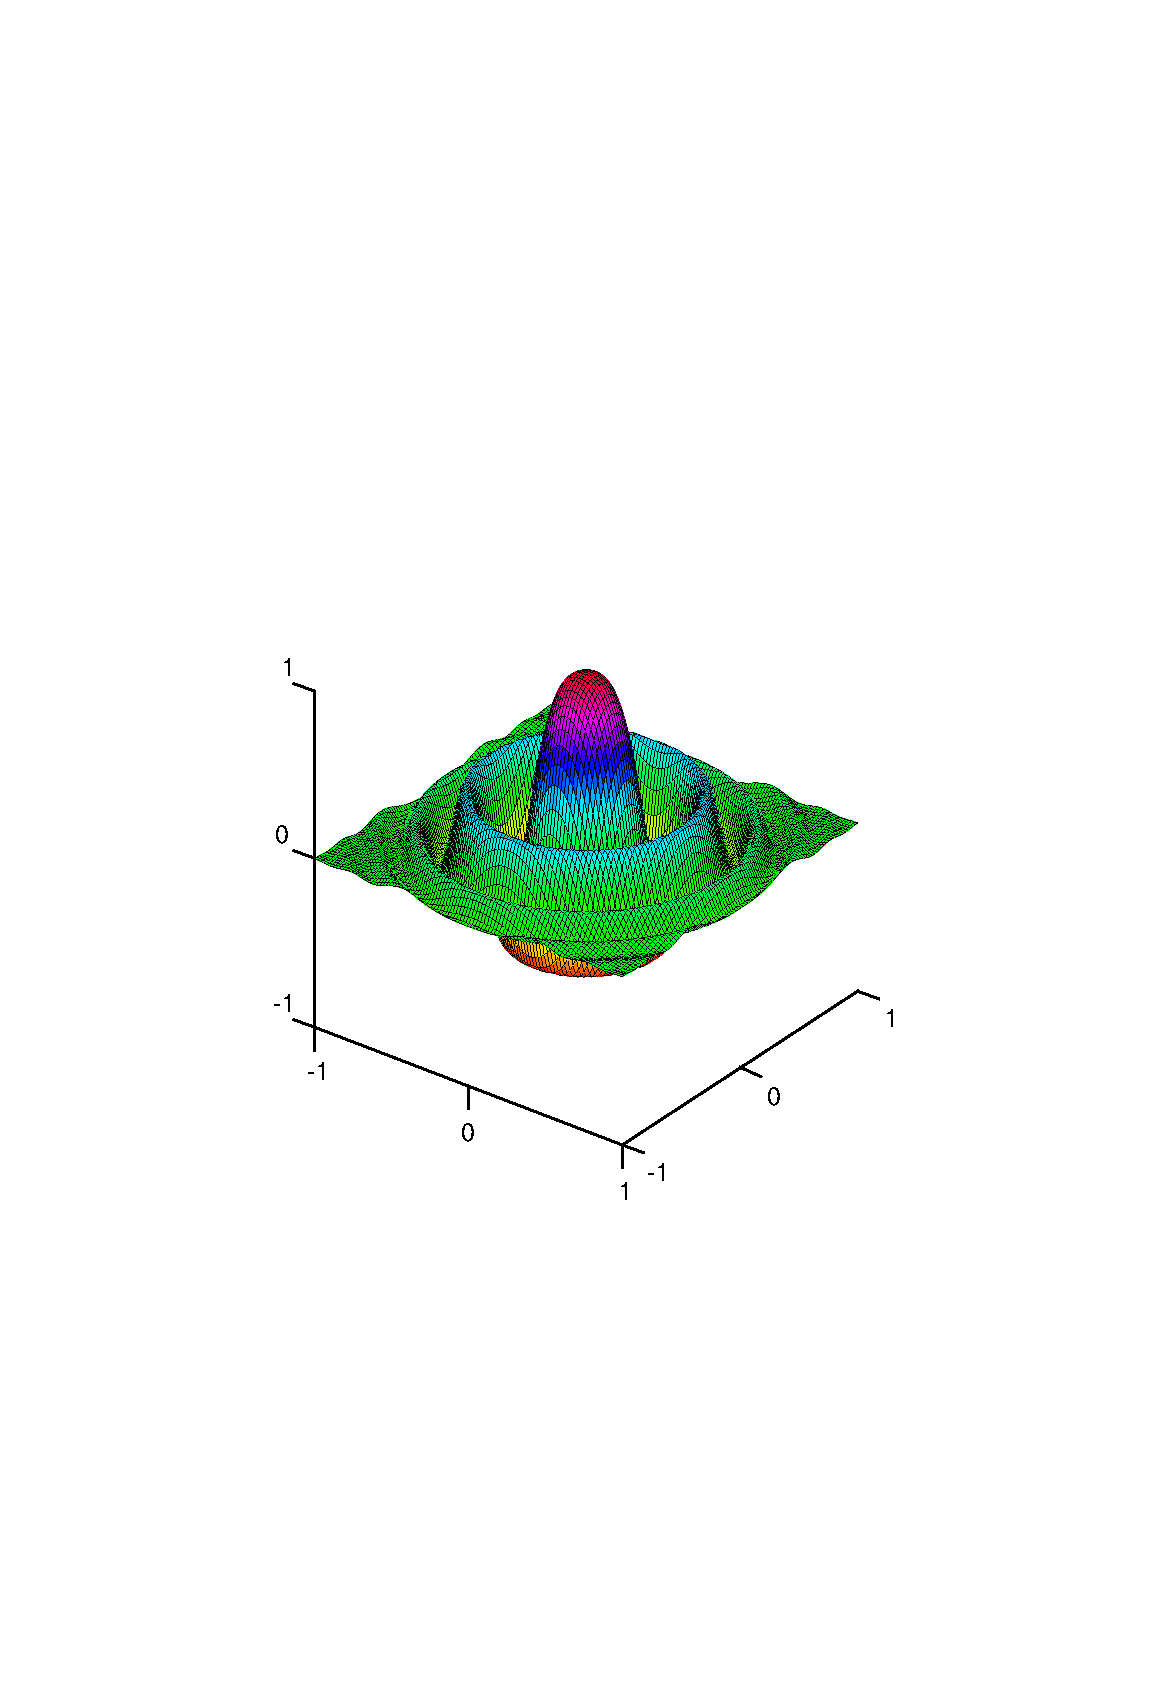
\includegraphics[width=12cm]{view1}
\caption{view1}
\end{DoxyImage}
 Next, we look at it as a 2\-D plot


\begin{DoxyVerbInclude}
--> surf(x,y,z);
--> axis equal
--> view(2)
\end{DoxyVerbInclude}


 
\begin{DoxyImage}
\includegraphics[width=12cm]{view2}
\caption{view2}
\end{DoxyImage}
 Finally, we generate a different view of the same surface.


\begin{DoxyVerbInclude}
--> surf(x,y,z);
--> axis equal
--> view(25,50);
\end{DoxyVerbInclude}


 
\begin{DoxyImage}
\includegraphics[width=12cm]{view3}
\caption{view3}
\end{DoxyImage}
 \hypertarget{handle_winlev}{}\section{W\-I\-N\-L\-E\-V Image Window-\/\-Level Function}\label{handle_winlev}
Section\-: \hyperlink{sec_handle}{Handle-\/\-Based Graphics} \hypertarget{vtkwidgets_vtkxyplotwidget_Usage}{}\subsection{Usage}\label{vtkwidgets_vtkxyplotwidget_Usage}
Adjusts the data range used to map the current image to the current colormap. The general syntax for its use is \begin{DoxyVerb}  winlev(window,level)
\end{DoxyVerb}
 where {\ttfamily window} is the new window, and {\ttfamily level} is the new level, or \begin{DoxyVerb}  winlev
\end{DoxyVerb}
 in which case it returns a vector containing the current window and level for the active image. \hypertarget{transforms_svd_Function}{}\subsection{Internals}\label{transforms_svd_Function}
Free\-Mat deals with scalar images on the range of {\ttfamily \mbox{[}0,1\mbox{]}}, and must therefor map an arbitrary image {\ttfamily x} to this range before it can be displayed. By default, the {\ttfamily image} command chooses \[ \mathrm{window} = \max x - \min x, \] and \[ \mathrm{level} = \frac{\mathrm{window}}{2} \] This ensures that the entire range of image values in {\ttfamily x} are mapped to the screen. With the {\ttfamily winlev} function, you can change the range of values mapped. In general, before display, a pixel {\ttfamily x} is mapped to {\ttfamily \mbox{[}0,1\mbox{]}} via\-: \[ \max\left(0,\min\left(1,\frac{x - \mathrm{level}}{\mathrm{window}} \right)\right) \] \hypertarget{variables_matrix_Examples}{}\subsection{Examples}\label{variables_matrix_Examples}
The window level function is fairly easy to demonstrate. Consider the following image, which is a Gaussian pulse image that is very narrow\-:


\begin{DoxyVerbInclude}
--> t = linspace(-1,1,256);
--> xmat = ones(256,1)*t; ymat = xmat';
--> A = exp(-(xmat.^2 + ymat.^2)*100);
--> image(A);
\end{DoxyVerbInclude}


The data range of {\ttfamily A} is {\ttfamily \mbox{[}0,1\mbox{]}}, as we can verify numerically\-:


\begin{DoxyVerbInclude}
--> min(A(:))

ans = 
 1.3839e-87 

--> max(A(:))

ans = 
    0.9969 
\end{DoxyVerbInclude}


To see the tail behavior, we use the {\ttfamily winlev} command to force Free\-Mat to map a smaller range of {\ttfamily A} to the colormap.


\begin{DoxyVerbInclude}
--> image(A);
--> winlev(1e-4,0.5e-4)
\end{DoxyVerbInclude}


The result is a look at more of the tail behavior of {\ttfamily A}. We can also use the winlev function to find out what the window and level are once set, as in the following example.


\begin{DoxyVerbInclude}
--> image(A);
--> winlev(1e-4,0.5e-4)
--> winlev

ans = 
 1.0000e-04 
\end{DoxyVerbInclude}
 \hypertarget{handle_xlabel}{}\section{X\-L\-A\-B\-E\-L Plot X-\/axis Label Function}\label{handle_xlabel}
Section\-: \hyperlink{sec_handle}{Handle-\/\-Based Graphics} \hypertarget{vtkwidgets_vtkxyplotwidget_Usage}{}\subsection{Usage}\label{vtkwidgets_vtkxyplotwidget_Usage}
This command adds a label to the x-\/axis of the plot. The general syntax for its use is \begin{DoxyVerb}  xlabel('label')
\end{DoxyVerb}
 or in the alternate form \begin{DoxyVerb}  xlabel 'label'
\end{DoxyVerb}
 or simply \begin{DoxyVerb}  xlabel label
\end{DoxyVerb}
 Here {\ttfamily label} is a string variable. You can also specify properties for that label using the syntax \begin{DoxyVerb}  xlabel('label',properties...) 
\end{DoxyVerb}
 \hypertarget{variables_struct_Example}{}\subsection{Example}\label{variables_struct_Example}
Here is an example of a simple plot with a label on the {\ttfamily x}-\/axis.


\begin{DoxyVerbInclude}
--> x = linspace(-1,1);
--> y = cos(2*pi*x);
--> plot(x,y,'r-');
--> xlabel('time');
\end{DoxyVerbInclude}


which results in the following plot.  
\begin{DoxyImage}
\includegraphics[width=12cm]{xlabel1}
\caption{xlabel1}
\end{DoxyImage}
 \hypertarget{handle_xlim}{}\section{X\-L\-I\-M Adjust X Axis limits of plot}\label{handle_xlim}
Section\-: \hyperlink{sec_handle}{Handle-\/\-Based Graphics} \hypertarget{vtkwidgets_vtkxyplotwidget_Usage}{}\subsection{Usage}\label{vtkwidgets_vtkxyplotwidget_Usage}
There are several ways to use {\ttfamily xlim} to adjust the X axis limits of a plot. The various syntaxes are \begin{DoxyVerb}   xlim
   xlim([lo,hi])   
   xlim('auto')
   xlim('manual')
   xlim('mode')
   xlim(handle,...)
\end{DoxyVerb}
 The first form (without arguments), returns a 2-\/vector containing the current limits. The second form sets the limits on the plot to {\ttfamily \mbox{[}lo,hi\mbox{]}}. The third and fourth form set the mode for the limit to {\ttfamily auto} and {\ttfamily manual} respectively. In {\ttfamily auto} mode, Free\-Mat chooses the range for the axis automatically. The {\ttfamily xlim('mode')} form returns the current mode for the axis (either {\ttfamily 'auto'} or {\ttfamily 'manual'}). Finally, you can specify the handle of an axis to manipulate instead of using the current one.

As an additional feature, you can now specify {\ttfamily inf} for a limit, and Free\-Mat will take that limit from the automatic set. So, for example {\ttfamily xlim(\mbox{[}10,inf\mbox{]})} will set the minimum for the x axis, but use the automatic value for the maximum. \hypertarget{variables_struct_Example}{}\subsection{Example}\label{variables_struct_Example}

\begin{DoxyVerbInclude}
--> x = linspace(-1,1);
--> y = sin(2*pi*x);
--> plot(x,y,'r-');
--> xlim  % what are the current limits?

ans = 
 -1  1 
\end{DoxyVerbInclude}


which results in  
\begin{DoxyImage}
\includegraphics[width=12cm]{xlim1}
\caption{xlim1}
\end{DoxyImage}
 Next, we zoom in on the plot using the {\ttfamily xlim} function


\begin{DoxyVerbInclude}
--> plot(x,y,'r-')
--> xlim([-0.2,0.2])
\end{DoxyVerbInclude}


which results in  
\begin{DoxyImage}
\includegraphics[width=12cm]{xlim2}
\caption{xlim2}
\end{DoxyImage}
 To demonstrate the infinite limits feature. Consider the following


\begin{DoxyVerbInclude}
--> plot(x,y,'r-');
--> xlim([0,inf])
\end{DoxyVerbInclude}


which results in  
\begin{DoxyImage}
\includegraphics[width=12cm]{xlim3}
\caption{xlim3}
\end{DoxyImage}
 \hypertarget{handle_ylabel}{}\section{Y\-L\-A\-B\-E\-L Plot Y-\/axis Label Function}\label{handle_ylabel}
Section\-: \hyperlink{sec_handle}{Handle-\/\-Based Graphics} \hypertarget{vtkwidgets_vtkxyplotwidget_Usage}{}\subsection{Usage}\label{vtkwidgets_vtkxyplotwidget_Usage}
This command adds a label to the y-\/axis of the plot. The general syntax for its use is \begin{DoxyVerb}  ylabel('label')
\end{DoxyVerb}
 or in the alternate form \begin{DoxyVerb}  ylabel 'label'
\end{DoxyVerb}
 or simply \begin{DoxyVerb}  ylabel label
\end{DoxyVerb}
 You can also specify properties for that label using the syntax \begin{DoxyVerb}  ylabel('label',properties...) 
\end{DoxyVerb}
 \hypertarget{variables_struct_Example}{}\subsection{Example}\label{variables_struct_Example}
Here is an example of a simple plot with a label on the {\ttfamily y}-\/axis.


\begin{DoxyVerbInclude}
--> x = linspace(-1,1);
--> y = cos(2*pi*x);
--> plot(x,y,'r-');
--> ylabel('cost');
\end{DoxyVerbInclude}


which results in the following plot.  
\begin{DoxyImage}
\includegraphics[width=12cm]{ylabel1}
\caption{ylabel1}
\end{DoxyImage}
 \hypertarget{handle_ylim}{}\section{Y\-L\-I\-M Adjust Y Axis limits of plot}\label{handle_ylim}
Section\-: \hyperlink{sec_handle}{Handle-\/\-Based Graphics} \hypertarget{vtkwidgets_vtkxyplotwidget_Usage}{}\subsection{Usage}\label{vtkwidgets_vtkxyplotwidget_Usage}
There are several ways to use {\ttfamily ylim} to adjust the Y axis limits of a plot. The various syntaxes are \begin{DoxyVerb}   ylim
   ylim([lo,hi])   
   ylim('auto')
   ylim('manual')
   ylim('mode')
   ylim(handle,...)
\end{DoxyVerb}
 The first form (without arguments), returns a 2-\/vector containing the current limits. The second form sets the limits on the plot to {\ttfamily \mbox{[}lo,hi\mbox{]}}. The third and fourth form set the mode for the limit to {\ttfamily auto} and {\ttfamily manual} respectively. In {\ttfamily auto} mode, Free\-Mat chooses the range for the axis automatically. The {\ttfamily ylim('mode')} form returns the current mode for the axis (either {\ttfamily 'auto'} or {\ttfamily 'manual'}). Finally, you can specify the handle of an axis to manipulate instead of using the current one.

As an additional feature, you can now specify {\ttfamily inf} for a limit, and Free\-Mat will take that limit from the automatic set. So, for example {\ttfamily ylim(\mbox{[}10,inf\mbox{]})} will set the minimum for the y axis, but use the automatic value for the maximum. \hypertarget{variables_struct_Example}{}\subsection{Example}\label{variables_struct_Example}

\begin{DoxyVerbInclude}
--> x = linspace(-1,1);
--> y = sin(2*pi*x);
--> plot(x,y,'r-');
--> ylim  % what are the current limits?

ans = 
   -0.9999    0.9999 
\end{DoxyVerbInclude}


which results in  
\begin{DoxyImage}
\includegraphics[width=12cm]{ylim1}
\caption{ylim1}
\end{DoxyImage}
 Next, we zoom in on the plot using the {\ttfamily ylim} function


\begin{DoxyVerbInclude}
--> plot(x,y,'r-')
--> ylim([-0.2,0.2])
\end{DoxyVerbInclude}


which results in  
\begin{DoxyImage}
\includegraphics[width=12cm]{ylim2}
\caption{ylim2}
\end{DoxyImage}
 To demonstrate the infinite limits feature. Consider the following


\begin{DoxyVerbInclude}
--> plot(x,y,'r-');
--> ylim([0,inf])
\end{DoxyVerbInclude}


which results in  
\begin{DoxyImage}
\includegraphics[width=12cm]{ylim3}
\caption{ylim3}
\end{DoxyImage}
 \hypertarget{handle_zlabel}{}\section{Z\-L\-A\-B\-E\-L Plot Z-\/axis Label Function}\label{handle_zlabel}
Section\-: \hyperlink{sec_handle}{Handle-\/\-Based Graphics} \hypertarget{vtkwidgets_vtkxyplotwidget_Usage}{}\subsection{Usage}\label{vtkwidgets_vtkxyplotwidget_Usage}
This command adds a label to the z-\/axis of the plot. The general syntax for its use is \begin{DoxyVerb}  zlabel('label')
\end{DoxyVerb}
 or in the alternate form \begin{DoxyVerb}  zlabel 'label'
\end{DoxyVerb}
 or simply \begin{DoxyVerb}  zlabel label
\end{DoxyVerb}
 Here {\ttfamily label} is a string variable. You can also specify properties for that label using the syntax \begin{DoxyVerb}  zlabel('label',properties...) 
\end{DoxyVerb}
 \hypertarget{variables_struct_Example}{}\subsection{Example}\label{variables_struct_Example}
Here is an example of a simple plot with a label on the {\ttfamily z}-\/axis.


\begin{DoxyVerbInclude}
--> t = linspace(0,5*pi);
--> x = cos(t);
--> y = sin(t);
--> z = t;
--> plot3(x,y,z,'r-');
--> view(3);
--> zlabel('time');
\end{DoxyVerbInclude}


which results in the following plot.  
\begin{DoxyImage}
\includegraphics[width=12cm]{zlabel1}
\caption{zlabel1}
\end{DoxyImage}
 \hypertarget{handle_zlim}{}\section{Z\-L\-I\-M Adjust Z Axis limits of plot}\label{handle_zlim}
Section\-: \hyperlink{sec_handle}{Handle-\/\-Based Graphics} \hypertarget{vtkwidgets_vtkxyplotwidget_Usage}{}\subsection{Usage}\label{vtkwidgets_vtkxyplotwidget_Usage}
There are several ways to use {\ttfamily zlim} to adjust the Z axis limits of a plot. The various syntaxes are \begin{DoxyVerb}   zlim
   zlim([lo,hi])   
   zlim('auto')
   zlim('manual')
   zlim('mode')
   zlim(handle,...)
\end{DoxyVerb}
 The first form (without arguments), returns a 2-\/vector containing the current limits. The second form sets the limits on the plot to {\ttfamily \mbox{[}lo,hi\mbox{]}}. The third and fourth form set the mode for the limit to {\ttfamily auto} and {\ttfamily manual} respectively. In {\ttfamily auto} mode, Free\-Mat chooses the range for the axis automatically. The {\ttfamily zlim('mode')} form returns the current mode for the axis (either {\ttfamily 'auto'} or {\ttfamily 'manual'}). Finally, you can specify the handle of an axis to manipulate instead of using the current one. \hypertarget{handle_zoom}{}\section{Z\-O\-O\-M Image Zoom Function}\label{handle_zoom}
Section\-: \hyperlink{sec_handle}{Handle-\/\-Based Graphics} \hypertarget{vtkwidgets_vtkxyplotwidget_Usage}{}\subsection{Usage}\label{vtkwidgets_vtkxyplotwidget_Usage}
This function changes the zoom factor associated with the currently active image. It is a legacy support function only, and thus is not quite equivalent to the {\ttfamily zoom} function from previous versions of Free\-Mat. However, it should achieve roughly the same effect. The generic syntax for its use is \begin{DoxyVerb}  zoom(x)
\end{DoxyVerb}
 where {\ttfamily x} is the zoom factor to be used. The exact behavior of the zoom factor is as follows\-: 
\begin{DoxyItemize}
\item {\ttfamily x$>$0} The image is zoomed by a factor {\ttfamily x} in both directions.  
\item {\ttfamily x=0} The image on display is zoomed to fit the size of the image window, but the aspect ratio of the image is not changed. (see the Examples section for more details). This is the default zoom level for images displayed with the {\ttfamily image} command.  
\item {\ttfamily x$<$0} The image on display is zoomed to fit the size of the image window, with the zoom factor in the row and column directions chosen to fill the entire window. The aspect ratio of the image is not preserved. The exact value of {\ttfamily x} is irrelevant.  
\end{DoxyItemize}\hypertarget{variables_struct_Example}{}\subsection{Example}\label{variables_struct_Example}
To demonstrate the use of the {\ttfamily zoom} function, we create a rectangular image of a Gaussian pulse. We start with a display of the image using the {\ttfamily image} command, and a zoom of 1.


\begin{DoxyVerbInclude}
--> x = linspace(-1,1,300)'*ones(1,600);
--> y = ones(300,1)*linspace(-1,1,600);
--> Z = exp(-(x.^2+y.^2)/0.3);
--> image(Z);
--> zoom(1.0);
\end{DoxyVerbInclude}


 
\begin{DoxyImage}
\includegraphics[width=12cm]{zoom1}
\caption{zoom1}
\end{DoxyImage}


At this point, resizing the window accomplishes nothing, as with a zoom factor greater than zero, the size of the image is fixed.

If we change the zoom to another factor larger than 1, we enlarge the image by the specified factor (or shrink it, for zoom factors {\ttfamily 0 $<$ x $<$ 1}. Here is the same image zoomed out to 60\%


\begin{DoxyVerbInclude}
--> image(Z);
--> zoom(0.6);
\end{DoxyVerbInclude}


 
\begin{DoxyImage}
\includegraphics[width=12cm]{zoom3}
\caption{zoom3}
\end{DoxyImage}


Similarly, we can enlarge it to 130\%


\begin{DoxyVerbInclude}
--> image(Z)
--> zoom(1.3);
\end{DoxyVerbInclude}


 
\begin{DoxyImage}
\includegraphics[width=12cm]{zoom4}
\caption{zoom4}
\end{DoxyImage}


The ``free'' zoom of {\ttfamily x = 0} results in the image being zoomed to fit the window without changing the aspect ratio. The image is zoomed as much as possible in one direction.


\begin{DoxyVerbInclude}
--> image(Z);
--> zoom(0);
--> sizefig(200,400);
\end{DoxyVerbInclude}


 
\begin{DoxyImage}
\includegraphics[width=12cm]{zoom5}
\caption{zoom5}
\end{DoxyImage}


The case of a negative zoom {\ttfamily x $<$ 0} results in the image being scaled arbitrarily. This allows the image aspect ratio to be changed, as in the following example.


\begin{DoxyVerbInclude}
--> image(Z);
--> zoom(-1);
--> sizefig(200,400);
\end{DoxyVerbInclude}


 
\begin{DoxyImage}
\includegraphics[width=12cm]{zoom6}
\caption{zoom6}
\end{DoxyImage}
 \hypertarget{handle_zplane}{}\section{Z\-P\-L\-A\-N\-E Zero-\/pole plot}\label{handle_zplane}
Section\-: \hyperlink{sec_handle}{Handle-\/\-Based Graphics} \hypertarget{vtkwidgets_vtkxyplotwidget_Usage}{}\subsection{Usage}\label{vtkwidgets_vtkxyplotwidget_Usage}
This function makes a zero-\/pole plot of a discrete-\/time system defined by its zeros and poles. The various syntaxes are \begin{DoxyVerb}    zplane(z,p)
\end{DoxyVerb}
 where {\ttfamily z} and {\ttfamily p} are the zeros and the poles of the system stored as column vectors, or \begin{DoxyVerb}    zplane(b,a)
\end{DoxyVerb}
 where {\ttfamily a} and {\ttfamily b} are the polynomial coefficients of the numerator and denominator stored as line vectors ({\ttfamily roots} is used to find the zeros and poles). The symbol {\ttfamily 'o'} represents a zero and the symbol {\ttfamily 'x'} represents a pole. The plot includes the unit circle for reference. Contributed by Paulo Xavier Candeias under G\-P\-L 